\documentclass[a4paper, twoside]{report}

%% Language and font encodings
\usepackage[english]{babel}
\usepackage[utf8x]{inputenc}
\usepackage[T1]{fontenc}

%% Sets page size and margins
\usepackage[a4paper,top=3cm,bottom=2cm,left=3cm,right=3cm,marginparwidth=1.75cm]{geometry}

%% Useful packages
\usepackage{adjustbox}
\usepackage{amsmath}
\usepackage{colortbl}
\usepackage{fancyhdr}
\usepackage{float}
\usepackage{graphicx}
\usepackage{listings}
\usepackage{url}
\usepackage{xcolor}
\usepackage{xskak}
\usepackage[super]{nth}
\usepackage[square]{natbib}
\usepackage[colorinlistoftodos]{todonotes}
\usepackage[parfill]{parskip}
\usepackage{hyperref}
\usepackage[nameinlink]{cleveref}

\title{Chess Puzzle Analysis}
\author{Mihhail Sorokin}
% Update supervisor and other title stuff in title/title.tex


\fancypagestyle{thesis}{
  \fancyhf{}
  \fancyhead[L]{\nouppercase{\leftmark}}
  \fancyhead[R]{\nouppercase{\rightmark}}
  \fancyfoot[LE,RO]{\thepage}
}

\definecolor[named]{ACMPurple}{cmyk}{0.55,1,0,0.15}
\definecolor[named]{ACMDarkBlue}{cmyk}{1,0.58,0,0.21}
\hypersetup{colorlinks,
linkcolor=ACMPurple,
citecolor=ACMPurple,
urlcolor=ACMDarkBlue,
filecolor=ACMDarkBlue
}

\widowpenalty10000
\clubpenalty10000

\pagestyle{thesis}

\begin{document}
\begin{titlepage}

\newcommand{\HRule}{\rule{\linewidth}{0.5mm}} % Defines a new command for the horizontal lines, change thickness here

%----------------------------------------------------------------------------------------
%	LOGO SECTION
%----------------------------------------------------------------------------------------


\includegraphics[width=8cm]{title/new_logo.eps}\\[1cm] % Include a department/university logo - this will require the graphicx package
 
%----------------------------------------------------------------------------------------

\center % Center everything on the page

%----------------------------------------------------------------------------------------
%	HEADING SECTIONS
%----------------------------------------------------------------------------------------

\textsc{\LARGE MEng Individual Project}\\[1.5cm] % Name of your university/college
\textsc{\Large Imperial College London}\\[0.5cm] % Major heading such as course name
\textsc{\large Department of Computing}\\[0.5cm] % Minor heading such as course title

%----------------------------------------------------------------------------------------
%	TITLE SECTION
%----------------------------------------------------------------------------------------
\makeatletter
\HRule \\[0.7cm]
{ \huge \bfseries \@title}\\[0.4cm] % Title of your document
\HRule \\[1.5cm]
 
%----------------------------------------------------------------------------------------
%	AUTHOR SECTION
%----------------------------------------------------------------------------------------

\begin{minipage}{0.4\textwidth}
\begin{flushleft} \large
\emph{Author:}\\
\@author % Your name
\end{flushleft}
\end{minipage}
~
\begin{minipage}{0.4\textwidth}
\begin{flushright} \large
\emph{Supervisor:} \\
Nicolas Wu \\[1.2em] % Supervisor's Name
\emph{Second Marker:} \\
Benjamin Hou % second marker's name
\end{flushright}
\end{minipage}\\[2cm]
\makeatother

% If you don't want a supervisor, uncomment the two lines below and remove the section above
%\Large \emph{Author:}\\
%John \textsc{Smith}\\[3cm] % Your name

%----------------------------------------------------------------------------------------
%	DATE SECTION
%----------------------------------------------------------------------------------------

{\large June 19, 2024}\\[2cm] % Date, change the \today to a set date if you want to be precise

\vfill % Fill the rest of the page with whitespace

\end{titlepage}



%%% DELETE COMMENTS LATER
\begin{abstract}

  This is the abstract placeholder. Hopefully this will get filled with
  proper text later.

\end{abstract}

\renewcommand{\abstractname}{Acknowledgements}
\begin{abstract}

  I would like to thank my supervisor, Nicolas Wu, for his guidance, time, and
  laissez-faire approach, which helped me thrive and enjoy this project.

  I express my gratitude to my friends and family who helped and supported
  me during this project, and the rest of my studies. 

\end{abstract}

\renewcommand{\abstractname}{Ethical Discussion}
\begin{abstract}

  This project has few, if any, ethical considerations that need to be made.
  The biggest concern is the source of the large datasets that may be used in
  this project, namely, the Lichess puzzle database. However, this database,
  along with all Lichess games is released under the Creative Commons CC0
  license -- meaning there is no restriction in its use.

  Each puzzle in this database contains a link to the game from which it was
  extracted, and this contains a Lichess username, which is deanonymising. In
  the initial data processing stage, these links are going to be removed, as
  they are unnecessary for the goals of the project.

  Another concern is the use of, and reference to specific chess games and
  the players in them, and various chess compositions\footnote{An
  artificially created position to showcase a uniquely challenging, rare, or
  otherwise interesting theme.} with their authors. Other than proper
  reference to the creators of the game or composition, there are no other
  considerations to be made.

\end{abstract}

\tableofcontents
%\listoffigures
%\listoftables

\chapter{Introduction}

Chess has long been analysed and enjoyed by both amateurs and professionals
alike, and with the birth of computer science, an algorithm, along with a
powerful enough computer to run it on, has been hunted for since at least
the 1950s.\cite{shannon} In 1997, Garry Kasparov, the strongest chess
Grandmaster at the time, was defeated by Deep Blue,\cite{deepBlue} and
in the world of chess, humans were displaced by machines forever. 

Despite this, chess remains a popular pastime for many people, with the largest
online chess website, \url{chess.com}, having over 160,000,000 total members
\cite{chesscomMembers}. Whilst chess engines compete at the superhuman level
with cutting-edge techniques, many average chess players refine their ability
with study of previous positions -- chess puzzles -- where the goal is to find
the critical move to punish the opponent's mistake and gain a decisive
advantage, or win the game immediately via checkmate. 

These puzzles seek to train the `tactics' element of one's chess ability, and
they can be categorised by the theme that occurs within them; some of these
include \emph{fork}ing enemy pieces with a knight, a well-known bishop
sacrifice known as the \emph{Greek gift sacrifice}, and many more, in addition
to their combinations.\cite{chessPatterns} This allows players to identify
which types of patterns they are often overlooking in real games, and to
selectively train to detect those. 

It is surprising that this categorisation is most often done manually, be it
via community voting,\cite{lichessPuzzles} or a list of rules that the puzzle
must satisfy to be classed one way or another.\cite{lichessTagger} This, along
with the infamous saying that `chess is 99\% tactics', suggests that there is a
need to explore this problem and provide in-depth categorisation of puzzles
(beyond what is currently the norm).

Chess Grandmasters often talk about the `feeling' of a position -- is it
possible to quantify this?

\section{Challenges}

(This section is blank... for now)

\section{Contributions}

(This one too)


\chapter{Background}\label{backgroundChapter}

After some brief motivation (\Cref{bg1}), this chapter covers some prerequisite
knowledge of chess concepts and important work in this topic.

The major chess notation formats are described (\Cref{bg2}), along with some
example puzzle themes (\Cref{bg3}) afterwards.

Closely related work that is critical to this project is also covered
(\Cref{bg4}). Related, but more distant work can be found at the end of the
report (\Cref{concWork}).

The Lichess puzzle database is introduced (\Cref{bg5}) and some initial data
exploration is performed to get a deeper understanding of this database.

\section{Importance of Puzzle Solving}\label{bg1}

The motivation behind solving chess puzzles, especially under time pressure, is
to improve one's pattern recognition abilities. \citet{thoughtAndChoice} showed
that chess players do not have a square-by-square recollection of the chess
board during play. Instead, they rely on interactions, and potential
interactions of pieces in a more abstract sense. This is made strikingly clear
by a professional chess player's drawing of a position from memory
(\Cref{deGrootFigure}).

\begin{figure}[H]
  \centering
  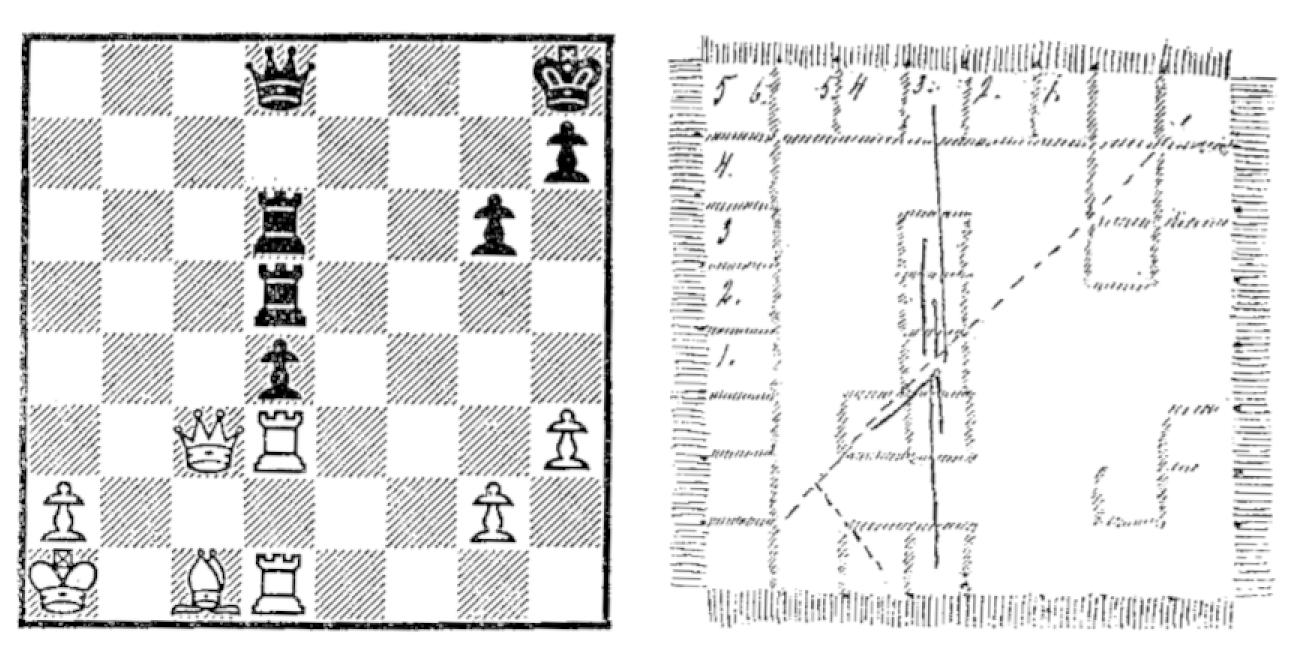
\includegraphics[width=0.6\textwidth]{background/img/deGroot.png}
  \caption{Taken from `Thought And Choice In Chess'
  \citep{thoughtAndChoice}.}
  \label{deGrootFigure}
\end{figure}

\citet{thoughtAndChoice} writes, ``the pieces themselves do not appear in the
drawing: rather the lines of force that go out from them''. This heuristic
allows expert human players to quickly hone in on the correct moves
\citep{bilalic2010mechanisms} and significantly reduces their search space,
when compared to a naive brute-force search, which is the most common strategy
for chess engines. When analysing positions, even the most basic chess engines
are able to calculate the most accurate line (except some pathological cases),
but they are unable to draw similarities between different positions.

Two sample chess positions are shown (\Cref{chess1,chess2}), featuring
\emph{back-rank checkmates} -- one of the first tactical patterns that a
beginner might learn. A castled king is forced to stay on the back-rank due to
the configuration of his men, and an opposing heavy piece exploits this
weakness by delivering checkmate. It is already non-trivial to programmatically
identify this type of tactic, as a checkmate delivered to a king on the back
rank is not necessarily a \emph{back-rank checkmate}.

Given positions similar to ones like these, how does one draw similarities
between the abstract relations of the heavy piece, king, and vulnerable back
rank?

\begin{figure}[H]
  \begin{minipage}[t]{0.475\textwidth}
    \centering
    \chessboard[setfen=6k1/5ppp/8/8/8/8/r4PPP/1R4K1 w - - 0 1]
    \caption{A trivial back-rank checkmate, White mates with
    \texttt{1.Rb8\#}.}
    \label{chess1}
  \end{minipage}
  \hspace{0.05\textwidth}
  \begin{minipage}[t]{0.475\textwidth}
    \centering
    \chessboard[setfen=6k1/5ppp/1p1Q4/p3p1B1/Pn4P1/1q6/1Pr4P/K6R w - - 1 2]
    \caption{White mates with \texttt{1.Qd8\#}.}
    \label{chess2}
  \end{minipage}
\end{figure}

\section{Chess Notation}\label{bg2}

For many decades, the standard for chess notation has been the Algebraic
System, where, generally speaking, moves are encoded by the piece abbreviation
(\texttt{Q} for queen, \texttt{K} for king, \texttt{N} for kNight) and a
reference to the destination square, which can be any letter \texttt{a-h} and
any number \texttt{1-8} \citep{fideNotation}. This report assumes that the
reader is familiar with the basic chess rules such as piece movement patterns.

When storing chess games and positions in a computer-readable format was
required, many formats were proposed by various people, but Portable Game
Notation (PGN) and Forsyth-Edwards Notation (FEN) stuck \citep{pgnNotation}.

\subsection{Portable Game Notation (PGN)}

PGN is a specific way to write chess moves in a text file. An example, taken
from Section 2.3 of the PGN Standard \citep{pgnNotation} is shown below. Along
with some metadata at the top of the file (player names, location, etc.\@), the
chess moves are written in algebraic notation, with an incrementing move
counter. In this example, Fischer played \texttt{e4} as his first move, with
Spassky responding with \texttt{e5}. The game ended in a draw on Spassky's
\nth{43} move.

\begin{verbatim}

[Event "F/S Return Match"]
[Site "Belgrade, Serbia JUG"]
[Date "1992.11.04"]
[Round "29"]
[White "Fischer, Robert J."]
[Black "Spassky, Boris V."]
[Result "1/2-1/2"]

1. e4 e5 2. Nf3 Nc6 3. Bb5 a6 4. Ba4 Nf6 5. O-O Be7 6. Re1 b5 7. Bb3 d6 8. c3
O-O 9. h3 Nb8 10. d4 Nbd7 11. c4 c6 12. cxb5 axb5 13. Nc3 Bb7 14. Bg5 b4 15.
Nb1 h6 16. Bh4 c5 17. dxe5 Nxe4 18. Bxe7 Qxe7 19. exd6 Qf6 20. Nbd2 Nxd6 21.
Nc4 Nxc4 22. Bxc4 Nb6 23. Ne5 Rae8 24. Bxf7+ Rxf7 25. Nxf7 Rxe1+ 26. Qxe1 Kxf7
27. Qe3 Qg5 28. Qxg5 hxg5 29. b3 Ke6 30. a3 Kd6 31. axb4 cxb4 32. Ra5 Nd5 33.
f3 Bc8 34. Kf2 Bf5 35. Ra7 g6 36. Ra6+ Kc5 37. Ke1 Nf4 38. g3 Nxh3 39. Kd2 Kb5
40. Rd6 Kc5 41. Ra6 Nf2 42. g4 Bd3 43. Re6 1/2-1/2 

\end{verbatim}

The main advantages of PGN are the ease with which it can be read by a human
\citep{pgnNotation} and, given its consistent structure, the simplicity of
parsing it programmatically. This led PGN to become widely adopted and
recognised by almost all chess software. However, a downside of PGN is that it
is difficult to retrieve a position at a given move -- it must be recalculated
by tracing the moves of the game from the start.

\subsection{Forsyth-Edwards Notation (FEN)}\label{fenSection}

An alternative notation used for static chess positions is FEN. This is much
more compact than PGN, as no metadata about the game is stored other than the
state of the board. The following FEN string encodes a standard position
arising from a King's Gambit.\footnote{An incredibly aggressive, all-or-nothing
opening for White. Also the authors' weapon of choice.} The board is also shown
in \Cref{chessKGA}.

\begin{verbatim}
rnbqkbnr/pppp1ppp/8/8/4Pp2/5N2/PPPP2PP/RNBQKB1R b KQkq - 1 3
\end{verbatim}

\begin{figure}[H]
  \centering
  \chessboard[setfen=rnbqkbnr/pppp1ppp/8/8/4Pp2/5N2/PPPP2PP/RNBQKB1R b KQkq -
  1 3]
  \caption{King's Gambit Accepted, King's Knight Gambit.}
  \label{chessKGA}
\end{figure}

In FEN, pieces have their standard one-letter names, but pawns are explicitly
referred to with \texttt{P} or \texttt{p}. The number of consecutive empty
squares on a rank is denoted by an integer between \texttt{1} and \texttt{8}.
The case of the letter dictates what colour the piece is: uppercase for white,
and lowercase for black. The arrangement of pieces is stored per rank,
left-to-right, with the first appearing rank in the string corresponding to
rank 8 on the board, and forward slashes delimiting the ranks. In the given
example, the \nth{6} rank is stored as \texttt{8}, meaning there are 8
consecutive empty squares on this rank. The \nth{4} rank is stored as
\texttt{4Pp2}, meaning there are 4 empty squares, followed by a white pawn,
then a black pawn, then 2 more empty squares.

The remaining characters store other information about the board. The single
\texttt{b} means it is Black to move; the string \texttt{KQkq} means White can
castle kingside (\texttt{K}) and queenside (\texttt{Q}), and Black can castle
both ways too (\texttt{kq}). If castling was not possible, this would be
denoted as \texttt{-}. The final 3 characters are the en
passant\footnote{French for `in passing'. A special move where a pawn that
advanced two squares can be captured by an enemy pawn as if it was on the
square behind. This is an unending source of confusion for beginner players.}
file, number of halfmoves since the last pawn move or capture\footnote{Used for
the fifty move draw rule.}, and the number of full moves played.

\subsection{Bitboards}

When implementing chess programs on a computer, neither PGN or FEN are
applicable as they are difficult and slow to analyse, being string-based.
Instead, there are a number of various numerical approaches to storing a chess
position, with bitboards being one of the bigger ones. One of the first
mentions of bitboards was by \citet{bitboardsRussian}.

Described informally, a bitboard is a collection of 12 64-bit integers, where
each integer corresponds to a piece type and colour. The bits of that integer
encode the position of a piece on the board: a piece on \texttt{h1} activates
the \nth{1} (least-significant) bit. Since modern processors utilise 64 bits,
this makes bitboards very fast -- especially when using other bitmaps to check
for piece attack maps and piece interactions. In fact, bitboards are used by
\citet{stockfishBitboard}, one of the strongest chess engines today.

\section{Examples of Chess Puzzle Themes}\label{bg3}

Some of the following positions are taken from \citet{chesscomTactics}.

\begin{figure}[H]
  \begin{minipage}{0.475\textwidth}
    \centering
    \chessboard[setfen=5r1k/4q1pp/3n2B1/1R5Q/8/7P/6P1/7K w - - 0 1]
  \end{minipage}
  \hspace{0.05\textwidth}
  \begin{minipage}{0.475\textwidth}
    \paragraph{Mate In One}White wins in one move with \texttt{1.Qxh7\#}. There
    are many variants of simple checkmates, some of which are covered below.
  \end{minipage}
\end{figure}

\begin{figure}[H]
  \begin{minipage}{0.475\textwidth}
    \centering
    \chessboard[setfen=6k1/5ppp/3r4/8/8/3q4/5PPP/R2B2K1 b - - 0 1]
  \end{minipage}
  \hspace{0.05\textwidth}
  \begin{minipage}{0.475\textwidth}
    \paragraph{Back-Rank Mate}Black wins with \texttt{1...Qxd1+ 2.Rxd1 Rxd1\#}.
    These positions occur very often when a king is castled, and the pawns
    surrounding the king on the \nth{2}/\nth{7} rank are preventing his escape
    to a different rank. A rook or queen delivers the checkmate
    single-handedly.
  \end{minipage}
\end{figure}

\begin{figure}[H]
  \begin{minipage}{0.475\textwidth}
    \centering
    \chessboard[setfen=q2r3k/6pp/8/3Q2N1/8/8/5PPP/6K1 w - - 0 1]
  \end{minipage}
  \hspace{0.05\textwidth}
  \begin{minipage}{0.475\textwidth}
    \paragraph{Smothered Mate}After \texttt{1.Nf7+ Kg8}, White wins by
    delivering a \emph{double~check} with \texttt{2.Nh6+}. Since Black is
    unable to remove both attacks on his king in one move, he is forced to move
    his king. \texttt{2...Kf8} leads to immediate mate with \texttt{3.Qf7\#},
    so Black runs to the corner with \texttt{2...Kh8}. The white queen is
    sacrificed with \texttt{3.Qg8+ Rxg8}, entombing the black king. The white
    knight delivers checkmate with \texttt{4.Nf7\#}.
  \end{minipage}
\end{figure}

\begin{figure}[H]
  \begin{minipage}{0.475\textwidth}
    \centering
    \chessboard[setfen= r2qk1nr/ppp2ppp/2np4/4p3/1b2P1b1/2NPBN2/PPP2PPP/R2QKB1R
    w KQkq - 2 6]
  \end{minipage}
  \hspace{0.05\textwidth}
  \begin{minipage}{0.475\textwidth}
    \paragraph{Absolute and Relative Pins}In this position, Black's bishops are
    pinning White's knights on \texttt{c3} and \texttt{f3}. The white knight on
    \texttt{c3} is under an \emph{absolute~pin} from the black bishop on
    \texttt{b4}, as moving it is illegal. The white knight on \texttt{f3} is
    under a \emph{relative~pin} from the other black bishop on \texttt{g4}.
    While moving this knight is legal, it is rarely done, as the bishop is then
    able to capture the white queen on \texttt{d1}.
  \end{minipage}
\end{figure}

\begin{figure}[H]
  \begin{minipage}{0.475\textwidth}
    \centering
    \chessboard[setfen=2r3k1/8/8/n1n2N2/8/8/1P6/6K1 w - - 0 1]
  \end{minipage}
  \hspace{0.05\textwidth}
  \begin{minipage}{0.475\textwidth}
    \paragraph{Fork}\emph{Fork}s are a type of \emph{double attack} and they
    come in multiple flavours, as all pieces can attack simulatenously. Perhaps
    the most common is the \emph{knight~fork}, an example of which is possible
    on the board with \texttt{1.Ne7+}, attacking both the black rook on
    \texttt{c8} and black king on \texttt{g8}. After moving the king, Black
    gives up the rook for a knight -- an unfavourable exchange.
    \\~\\
    The double pawn advance \text{1.b4} is also a \emph{fork}. Black's knights
    are attacked and even though they are able to defend each other, Black
    cannot move both to safety. One of them will be captured by the pawn.
  \end{minipage}
\end{figure}

\begin{figure}[H]
  \begin{minipage}{0.475\textwidth}
    \centering
    \chessboard[setfen=r2qkbnr/ppp2ppp/2np4/4N3/2B1P3/2N4P/PPPP1PP1/R1BbK2R w
    KQkq - 0 7]
  \end{minipage}
  \hspace{0.05\textwidth}
  \begin{minipage}{0.475\textwidth}
    \paragraph{Attack On \texttt{f2}/\texttt{f7}}The \texttt{f2} and
    \texttt{f7} squares are very vulnerable for White and Black, respectively.
    At the beginning of the game, these squares are defended only by the king.
    If neglected, a quick attack, or even a \emph{sacrifice}, can be fatal.
    \\~\\
    In this position, after sacrificing the queen, White's bishop can capture
    the weak pawn on \texttt{f7}, leading to \texttt{1.Bxf7+ Ke7 2.Nd5\#}. 
  \end{minipage}
\end{figure}


\section{Existing Work}\label{relatedWorkSection}\label{bg4}

\subsection{Chess Board Representation}

\paragraph{CNNs For Identifying Winning Positions}\citet{chessCNN} explores
the effectiveness of neural networks to analyse whether a chess position is
winning or losing, without creating specific look-ahead algorithms. This is a
very challenging task, but as part of the analysis, the author proposed
manually encoded features to a convolutional neural network (CNN) to help
identify strong patterns within the position. 

Some of these include extra features if the opponent is in check, specifying
the squares controlled by a piece exerting a pin on a different piece, centre
control, and vulnerable squares \citep{chessCNN}. These are well known
heuristics that are often taught to beginner-intermediate chess players, and
the author claims that these additional layers are ``extremely representative
of the chess positions'', and cause the CNN to outperform a naive,
fully-connected neural network.

\paragraph{Automatic Embedding}\citet{chess2vec} investigate and report on
their results in finding $d$-dimensional vector representations of the standard
way to represent a chess board in machine learning -- a bitboard, which is
equivalent to a $8\times8\times12$ binary tensor. 

The authors make the observation that this represents each chess square as a
12-dimensional vector, which has no information about the rest of the board. By
adding a board hash, they modify the piece layers, making their vector
representations depend on the board state. With this method, \citet{chess2vec}
claim to predict $8.8\%$ of Stockfish moves correctly, which is an impressive
statistic given no chess logic or ruleset was explicitly implemented.

The results of these works served as initial inspiration for the design of the
deep learning model (\Cref{mlS21}).

\subsection{Puzzle Type and Difficulty Prediction}\label{typeAndDifficultyReview}

\paragraph{Detecting Whether a Successful Tactic
Exists}\citet{middleGamePatterns} report their findings on a program to
identify the \emph{Greek gift sacrifice} tactic in chess
middlegames.\footnote{The phase of the chess game where most pieces are
developed and the kings are positioned away from danger.} They found success,
partly thanks to their detailed representation of the board, where each square
is represented by 71 binary attribites \citep{middleGamePatterns} to encode the
piece on the square and the possible squares which are reachable by this piece. 

These attributes were also supplemented by 59 other binary attribites which
were devised by expert chess players, and represent the more complex, but still
quantifiable relationships. These include open files, control of vulnerable
squares, and piece activity, among others.

\citet{middleGamePatterns} achieved an 87.7\% classification performance on
detecting whether a position features a successful \emph{Greek gift sacrifice}
on relatively small ($<200$ positions) datasets. 

\paragraph{Meaningful Search Trees}\citet{chessTrees} explore estimation of
difficulty of chess problems in this paper. By using a powerful chess engine,
they generate a tentative move tree of forcing or winning moves in a given
position, mirroring the process of calculating a variation for a chess player. 

By creating higher level metrics based off these trees (e.g. branching factor,
piece variety, move distances) and applying standard statistical machinery, the
authors are able to categorise the puzzles into various difficulty levels with
some success.

Their unique `meaningful search tree' \citep{chessTrees} approach to analysing
chess puzzle moves is full of potential, and is this is built upon and explored
further with the tree-based approach (\Cref{treeS12}).

\paragraph{Static and Dynamic Similarity}In their thesis, \citet{chessMotifs}
develop a method to retrieve similar chess positions among a variety of
tactically sharp examples. Building upon the naive `static' similarity (piece
locations, pawn structure, etc.\@), they implement various `dynamic' similarity
metrics (whether captures occur, attacks happen, sacrifices happen, etc.\@ in
the optimal move chain). It is well known \citep{thoughtAndChoice,
bilalic2010mechanisms} that chess players often think about positions in this
dynamic way. This is further reinforced by an example given in the thesis,
where a small static perturbation causes previously dynamically similar
positions to have nothing in common \citep{chessMotifs}.

Importantly, their results are successful: when a chess expert was asked to
identify similar positions, they chose the same ones that the program of
\cite{chessMotifs} did. While this is not a faultless evaluation metric, it
shows that this approach works. The ideas of this thesis are the foundation of
the distance function used in the tree-based approach (\Cref{treeS13}).

\section{Lichess Puzzle Database}\label{lichessPuzzlesSection}\label{bg5}

Lichess (\url{https://lichess.org}) is a popular, open-source chess website
which often publishes the games that have been played by players of all skill
levels on it. As part of this, Lichess has published over 3.6 million rated and
tagged puzzle positions \citep{lichessPuzzles}. To generate these, 300 million
games were analysed with a powerful chess engine to find critical positions in
which a move must be played to capitalise on the opponent's mistake. These
puzzles were initially tagged to 60 manually created themes \citep{lichessXML},
which were identified by a Python script \citep{lichessTagger}.

As various users of the site solved the puzzles, and manually highlighted the
themes that they thought occured in the puzzle, the ratings and tags of the
puzzle database evolved until their current state.

\subsection{Format}

These puzzles are stored in FEN format, with a reference to the game where they
appeared. They also contain the solution as a sequence of moves, the tactics
tags \citep{lichessXML}, and the puzzle rating, along with other metadata.

An example puzzle string is shown below. This puzzle is also shown visually in
\Cref{puzzle1,puzzle2}.

\begin{verbatim}
q3k1nr/1pp1nQpp/3p4/1P2p3/4P3/B1PP1b2/B5PP/5K2 b k - 0 17,
e8d7 a2e6 d7d8 f7f8,1760,80,83,72,mate mateIn2 middlegame short,
https://lichess.org/yyznGmXs/black#34,
Italian_Game Italian_Game_Classical_Variation
\end{verbatim}

\begin{figure}[H]
  \begin{minipage}[t]{0.475\textwidth}
    \centering
    \chessboard[setfen=q3k1nr/1pp1nQpp/3p4/1P2p3/4P3/B1PP1b2/B5PP/5K2 b k -
    0 17]
    \caption{Position given by the FEN string above.}
    \label{puzzle1}
  \end{minipage}
  \hspace{0.05\textwidth}
  \begin{minipage}[t]{0.475\textwidth}
    \centering
    \chessboard[setfen=q5nr/1ppknQpp/3p4/1P2p3/4P3/B1PP1b2/B5PP/5K2 w - - 1
    18]
    \caption{Black blunders: \texttt{17...Kd7}. This position is given to
    the end user as a puzzle to be solved with forcing moves. Checkmate is
    imminent with \texttt{18.Be6+ Kd8 19.Qf8\#}.}
    \label{puzzle2}
  \end{minipage}
\end{figure}

Processing these is a trivial task with one small detail: the given FEN strings
are the state of the game right before the critical blunder is played by the
opposing site. This means the puzzle, as shown to the user, is the position
after the first move has been played. Fortunately, processing this data is made
simple with the \texttt{python-chess} library \citep{pythonChess}.

\subsection{Data Exploration}\label{lichessDataExpl}

The Lichess puzzle database has approximately 3.8 million rated and tagged
chess puzzles. Initially, they were automatically processed
\citep{lichessTagger}, but were then refined with user feedback
\citep{lichessPuzzles}. This also allowed the puzzles to obtain a rating, which
is indicative of its difficulty \citep{lichessPuzzles}.

Overall, there are 60 various puzzle themes \citep{lichessXML}.
\Cref{dataThemeCounts} shows the counts of each theme in all of the contained
puzzles. It should be noted that some themes are mutually exclusive (a
checkmate puzzle cannot be both \emph{mate-in-one} and \emph{mate-in-two}).

The most common puzzle themes are the most general ones -- specifically
\texttt{short}, \texttt{middlegame}, and \texttt{endgame}. There is a lot of
variation in how frequent the various patterns are, which is a natural
consequence of the game.

\begin{figure}
  \centering
  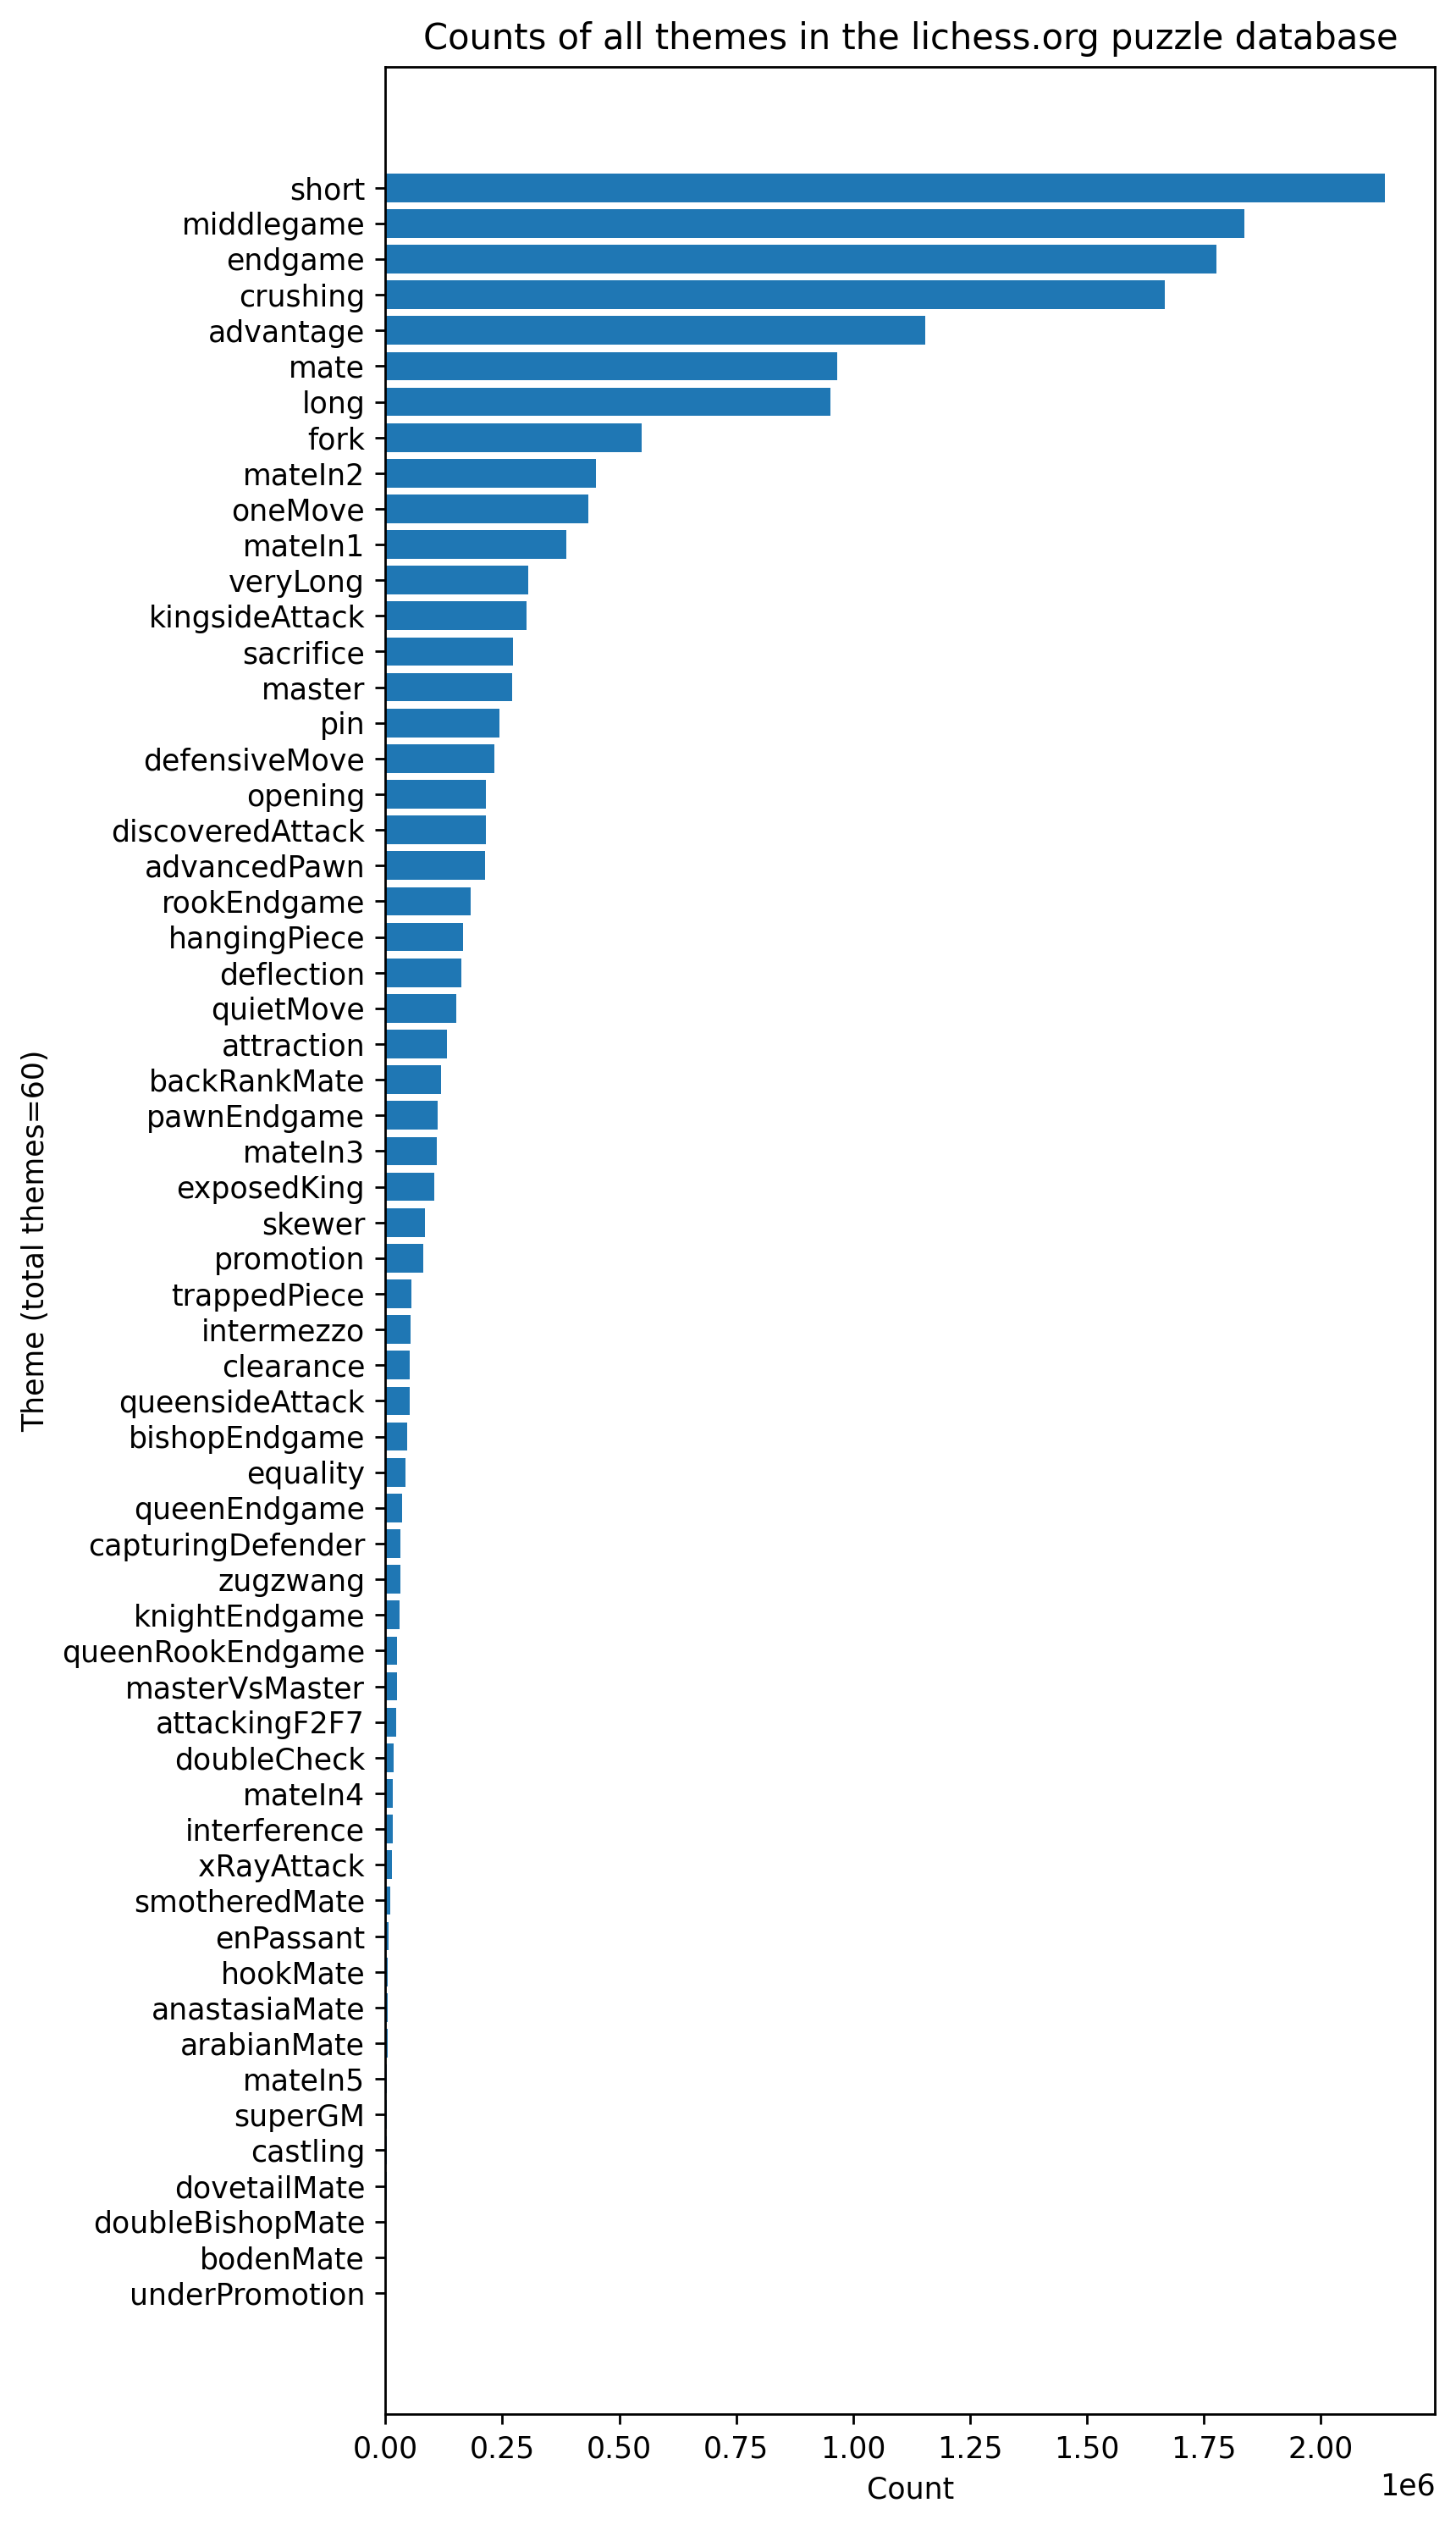
\includegraphics[width=0.9\linewidth]{project/img/puzzle_theme_counts.png}
  \caption{Frequency of puzzle themes in the Lichess puzzle database
  \citep{lichessPuzzles}.}
  \label{dataThemeCounts}
\end{figure}

\Cref{dataHistogram} shows the distribution of ratings across the chess
puzzles. These ratings are only appropriate within this dataset, and cannot be
compared to ratings of puzzles on other chess websites. The puzzle ratings are
symmetric about the mean, and this is of course a result of the Glicko2 rating
system, developed by \citet{glicko}.

When analysing the rating distribution by theme, an expected behaviour occurs.
Some chess tactics patterns are considerably simpler to spot, meaning a weaker
player is able to solve the puzzle with that theme. Therefore some puzzle
themes, \emph{back-rank mate} (\Cref{puzzle3}), for example, have lower-rated
puzzles when compared to puzzles featuring a \emph{trapped piece}
(\Cref{puzzle4}) or \emph{defensive move}.\footnote{Notoriously difficult for
humans, who are usually much better at aggression than
defense.\footnotemark}\footnotetext{In chess.}

\begin{figure}[H]
  \begin{minipage}[t]{0.475\textwidth}
    \centering
    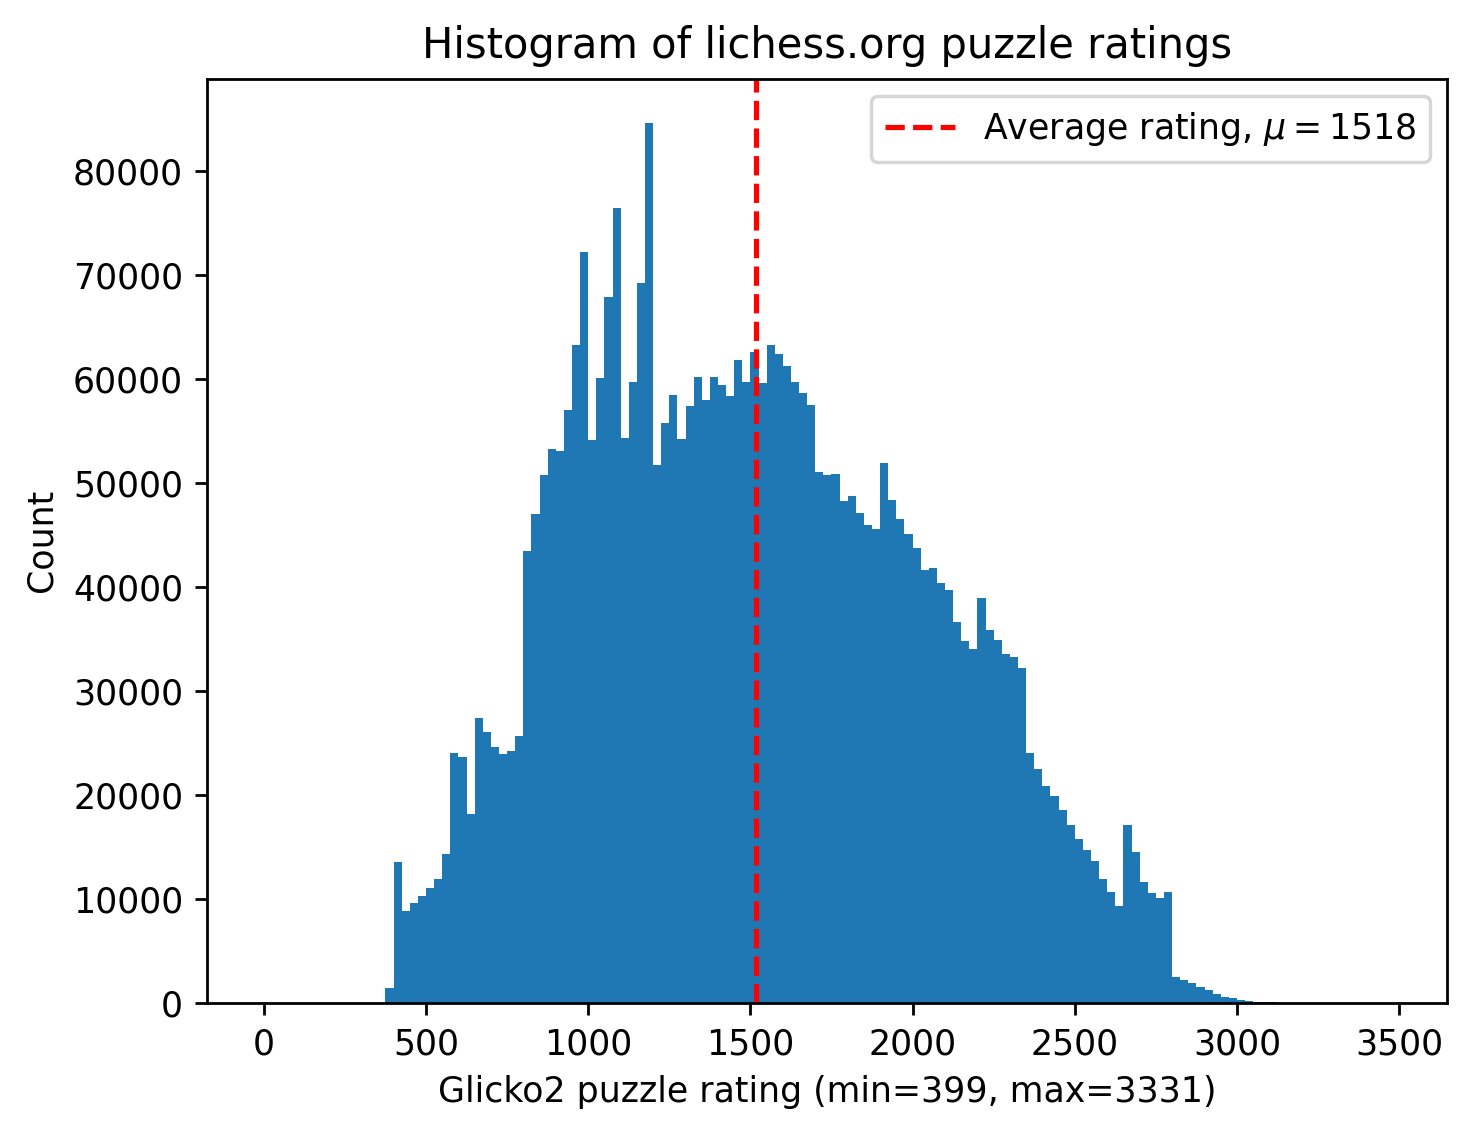
\includegraphics[width=\textwidth]{project/img/puzzle_histogram.png}
    \caption{Distribution of Lichess puzzle ratings.}
    \label{dataHistogram}
  \end{minipage}
  \hspace{0.05\textwidth}
  \begin{minipage}[t]{0.475\textwidth}
    \centering
    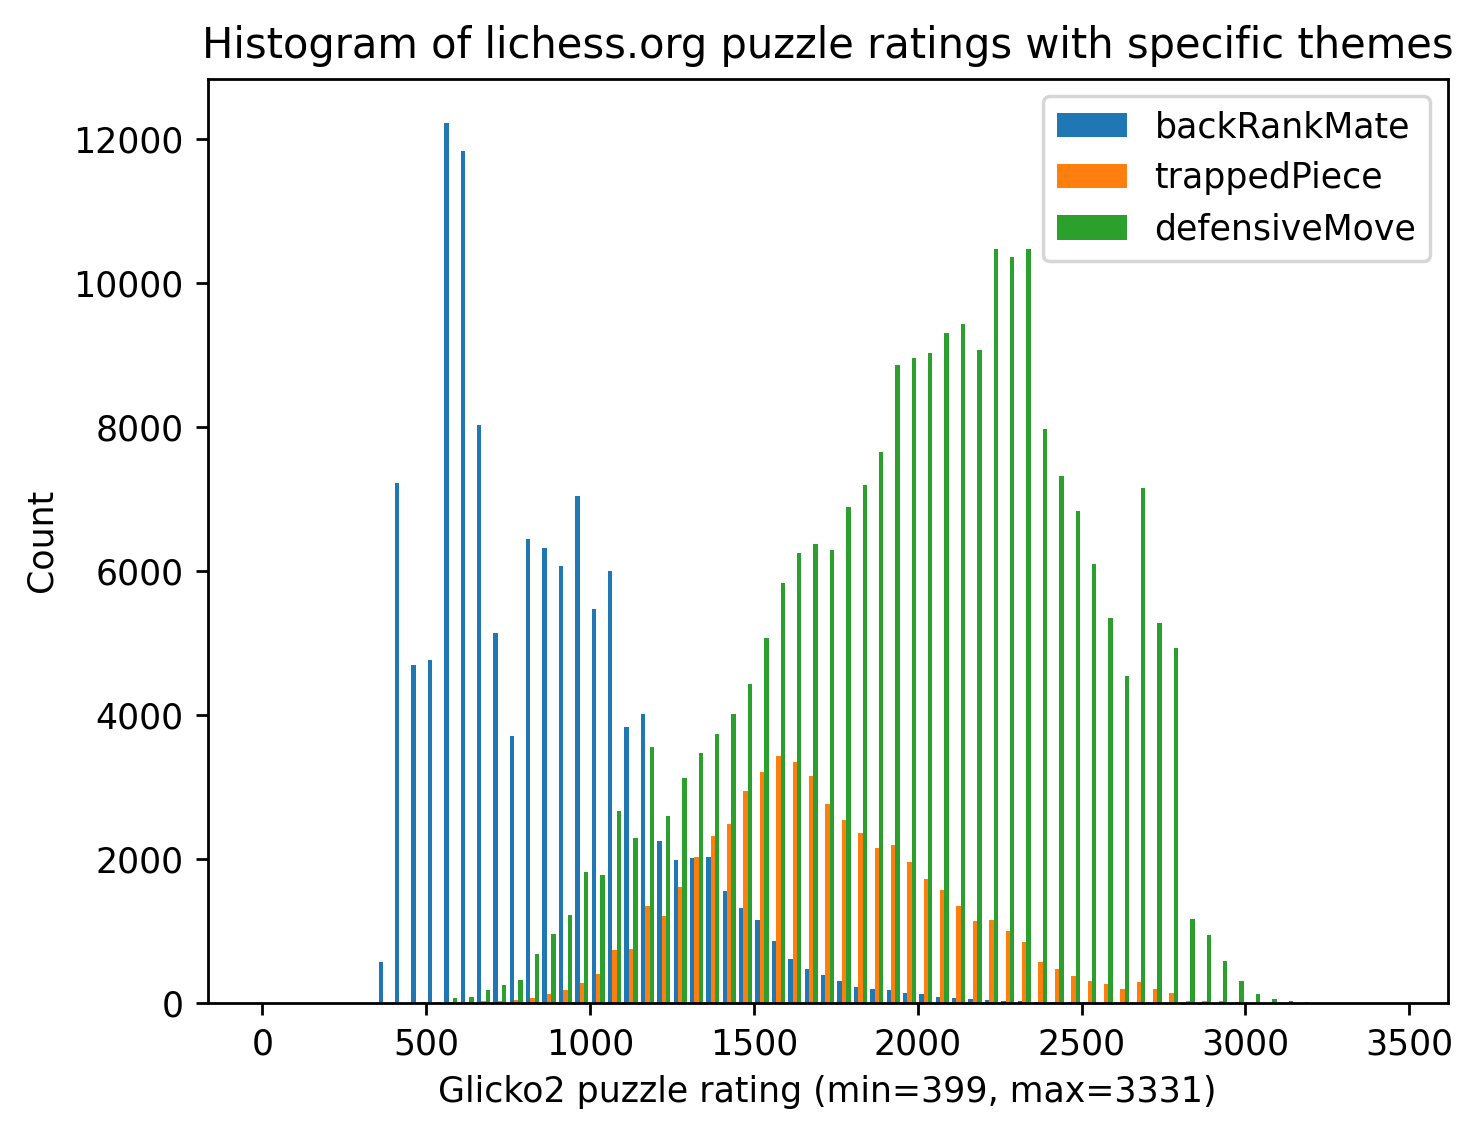
\includegraphics[width=\textwidth]
    {project/img/puzzle_theme_histograms.png}
    \caption{Distribution of Lichess puzzle ratings with a specific theme.}
    \label{dataThemeHistogram}
  \end{minipage}
\end{figure}

\begin{figure}[H]
  \begin{minipage}[t]{0.475\textwidth}
    \centering
    \chessboard[setfen=6k1/5ppp/r1p5/p1n1rP2/8/2P2N1P/2P3P1/3R2K1 w - - 0
    22]
    \caption{\textbf{Kenan2345 -- gandie}, lichess.org Blitz game, move 22. 
    Black loses to \texttt{22.Rd8+}.}
    \label{puzzle3}
  \end{minipage}
  \hspace{0.05\textwidth}
  \begin{minipage}[t]{0.475\textwidth}
    \centering
    \chessboard[setfen=2rq1rk1/7p/1n4pb/1R2Q3/pPpP1P2/P1B5/3N2PP/2R3K1 b -
    - 0 31]
    \caption{\textbf{mhabib -- Sarg0n}, lichess.org Blitz game, move 31.
    White loses his queen after \texttt{31...Re8}, as the queen has no
    safe squares to escape to.}

    \label{puzzle4}
  \end{minipage}
\end{figure}


\chapter{The Deep Learning Approach}\label{mlChapter}

This chapter describes and analyses a novel approach to the specific problem of
chess puzzle classification, inspired by the recent advancements in the field
of natural language processing.

The justification for why transformers may work, along with a slightly more
formal problem statement, is outlined (\Cref{mlS0}).

The data pipeline is then discussed (\Cref{mlS1}), starting with the bitboard
encoding (\Cref{mlS11}) and ending with the training, validation, and testing
splits (\Cref{mlS12}).

The process of creating the model is then described in detail (\Cref{mlS2}),
including architecture (\Cref{mlS21}), training setup (\Cref{mlS23}), and
hyperparameter selection (\Cref{mlS22}).

Finally, the internals of the model are explored (\Cref{mlS3}) by visualising
the input for specific chess boards (\Cref{mlS32}). These are then discussed
(\Cref{mlS33}). The model is fully evaluated in \Cref{evalChapter}, \nameref{evalChapter}.


\section{Overview}\label{mlS0}

\subsection{Why Should This Work?}

Earlier (\Cref{bg4}), some papers were highlighted which seek to find new ways
to build on the naive bitboard representation by exploring new embeddings for
chess pieces and chess board squares. These publications make the crucial point
that chess pieces influence each other on the board, and this has to be taken
into account, whether it is by creating extra features to represent pins and
central square control \citep{chessCNN}, open files and attack squares
\citep{middleGamePatterns}, or the hash of the entire chess board
\citep{chess2vec}.

Continuing along the `chess board as a $N\times64$ vector' path and, given how
puzzle tactics rely on the interaction of pieces' locations and attack squares,
it seems natural to explore whether the transformer architecture, as described
in the infamous paper `Attention Is All You Need' by \citet{attention}, can
help extract patterns from static chess positions, which can then be used in
the downstream task of puzzle classification and difficulty rating. A
correspondence can be drawn between how words/tokens influence each other in
the transformer encoder (\Cref{attentionLinks}) and how chess pieces/squares
interact on the 64 squares (\Cref{chessPuzzleLinks}).

Applying transformers to chess has been done before by
\citet{chessTransformer}, whose work is reviewed at the end of the report
(\Cref{chessTransformerSection}), but treating individual chess board squares
as embeddings of tokens/words has not been previously explored.

\begin{figure}[H]
  \begin{minipage}{0.4\textwidth}
    \centering
    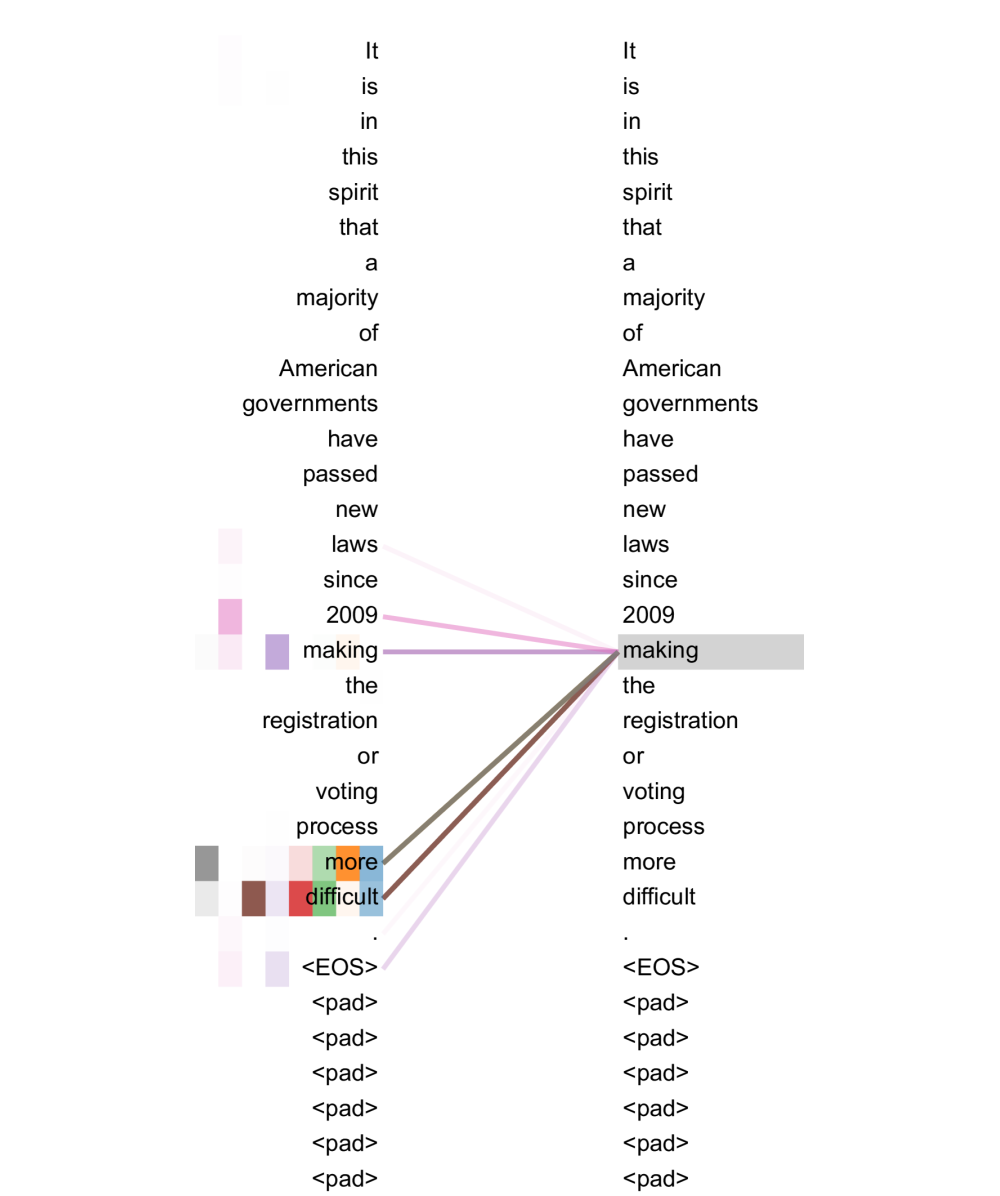
\includegraphics[width=\textwidth]{project/img/attention.png}
    \caption{Attention mechanism in the encoder. Taken from
    `Attention Is All You Need' \citep{attention}.}
    \label{attentionLinks}
  \end{minipage}
  \hspace{0.05\textwidth}
  \begin{minipage}{0.475\textwidth}
    \centering
    \chessboard[setfen=r3r1n1/bp6/p2p2kp/3N4/2P3n1/1PQ3Pq/P4P2/4RRK1 w - - 0 1,
    pgfstyle=border,markfields={d5},
    pgfstyle=straightmove,
    markmoves={f4-g6,f4-h3,c7-a8,c7-e8,d5-c7,d5-f4},
    pgfstyle=color,opacity=0.5,
    color=blue,markfields={f4,c7},
    pgfstyle=color,opacity=0.5,
    color=red,markfields={h3,g6,a8,e8}]

    \caption{Example of a relationship between chess pieces and squares.}

    \label{chessPuzzleLinks}
  \end{minipage}
\end{figure}

\subsection{Problem Statement}

Given a dataset with $N$ distinct puzzle labels ($N=60$ for the Lichess puzzle
database), each label is assigned an index $i$ and a binary $N$-dimensional
vector $x$ is formed such that $x[i]=1$ iff the puzzle is labelled with that
label. This is a common technique to reduce a multi-label classification into a
more tractable problem.

With this, a model is to be developed that, given a stationary chess position
in FEN (\Cref{fenSection}), returns a prediction for this
position's puzzle label vector.

\section{The Data}\label{mlS1}

\subsection{Bitboard Encoding}\label{mlS11}

The string-based FEN is naturally incompatible for machine learning models. To
solve this, $12\times8\times8$ chess bitboards are used, which was also seen in
the work of \citet{chess2vec}. Slightly more formally, the element $B[z, x, y]$
of bitboard $B$ is $1$ iff there is a piece $z \in \{\texttt{p}, \texttt{P},
\texttt{n}, \texttt{N}, \texttt{b}, \texttt{B}, \texttt{r}, \texttt{R},
\texttt{q}, \texttt{Q}, \texttt{k}, \texttt{K}\}$\footnote{FEN-inspired --
white pieces are uppercase, black pieces are lowercase.} at rank $x \in
\{\texttt{1}, \texttt{2}, \texttt{3}, \texttt{4}, \texttt{5}, \texttt{6},
\texttt{7}, \texttt{8}\}$}, file $y \in \{\texttt{a}, \texttt{b}, \texttt{c},
\texttt{d}, \texttt{e}, \texttt{f}, \texttt{g}, \texttt{h}\}$.

This method has 2 major downsides: there is no way to distinguish if en passant
or castling is legal. However, there are only 5644 (0.14\%) puzzles tagged as
`en passant' in the Lichess database, and 2029 (0.053\%) tagged as `castling'
-- this is a negligible number and the rare situations where a tactic would be
changed by an impossible en passant/castle being possible can be ignored.

To make learning easier (and to decrease implementation complexity), all chess
positions are transformed to be from the perspective of White. This has
negligible additional overhead, as it requires a simple mirror and has great
benefits, as the model no longer needs to distinguish between White-to-move and
Black-to-move puzzles.

\subsection{Train/Validation/Test Split}\label{mlS12}

As is standard in statistical learning problems, the dataset is split into 3
non-overlapping subsets: a training set containing 60\% of the data, a
validation set containing 20\% of the data, and a test set with the remaining
20\% of the data. The training set is used to train the model, the validation
set is used to find the optimal set of hyperparameters (\Cref{mlS22}), and the
test set is withheld until the final evaluation section to get an estimate of
the model's performance on unseen data. 

\section{The Model}\label{mlS2}

\subsection{Architecture}\label{mlS21}

The overview of the model architecture is shown in \Cref{MLDiagram}. 

At first, there is a pointwise convolution to expand the 12 piece bitboards to
64 channels. This is followed by a stack of `embedding layers'. Each embedding
layer consists of an $8\times8$ convolution with circular padding, to allow
every chess square access to other chess squares. The channel count is kept
constant within every embedding layer. Between each of the four embedding
layers lies a pointwise convolution which doubles the channel count. The number
of layers and layer channels are defined at the creation of the model and are
optimised during the hyperparameter search stage (\Cref{mlS22}). Every
convolution layer is followed by the rectified linear unit (ReLU) activation
and batch normalisation \citep{ioffe2015batch}.

This embeds the 64 chess squares in a 512-dimensional space. The 2D structure
of the board is flattened, and passed through 8 standard transformer encoder
\citep{attention} layers, featuring self-attention and a feedforward layer. The
internal dropout and activation of the transformer encoder layer was kept
default (0.1 and ReLU, respectively). The feedforward layer size was optimised
(\Cref{mlS22}).

Finally, the entire output is flattened and a fully connected layer connects
this to the 60 output neurons, which correspond to each of the 60 Lichess
puzzle database themes. As the themes are not mutually exclusive, softmax
cannot be used, so sigmoid activation is used to map the outputs to the range
to $(0, 1)$.

\begin{figure}[H]
  \centering
  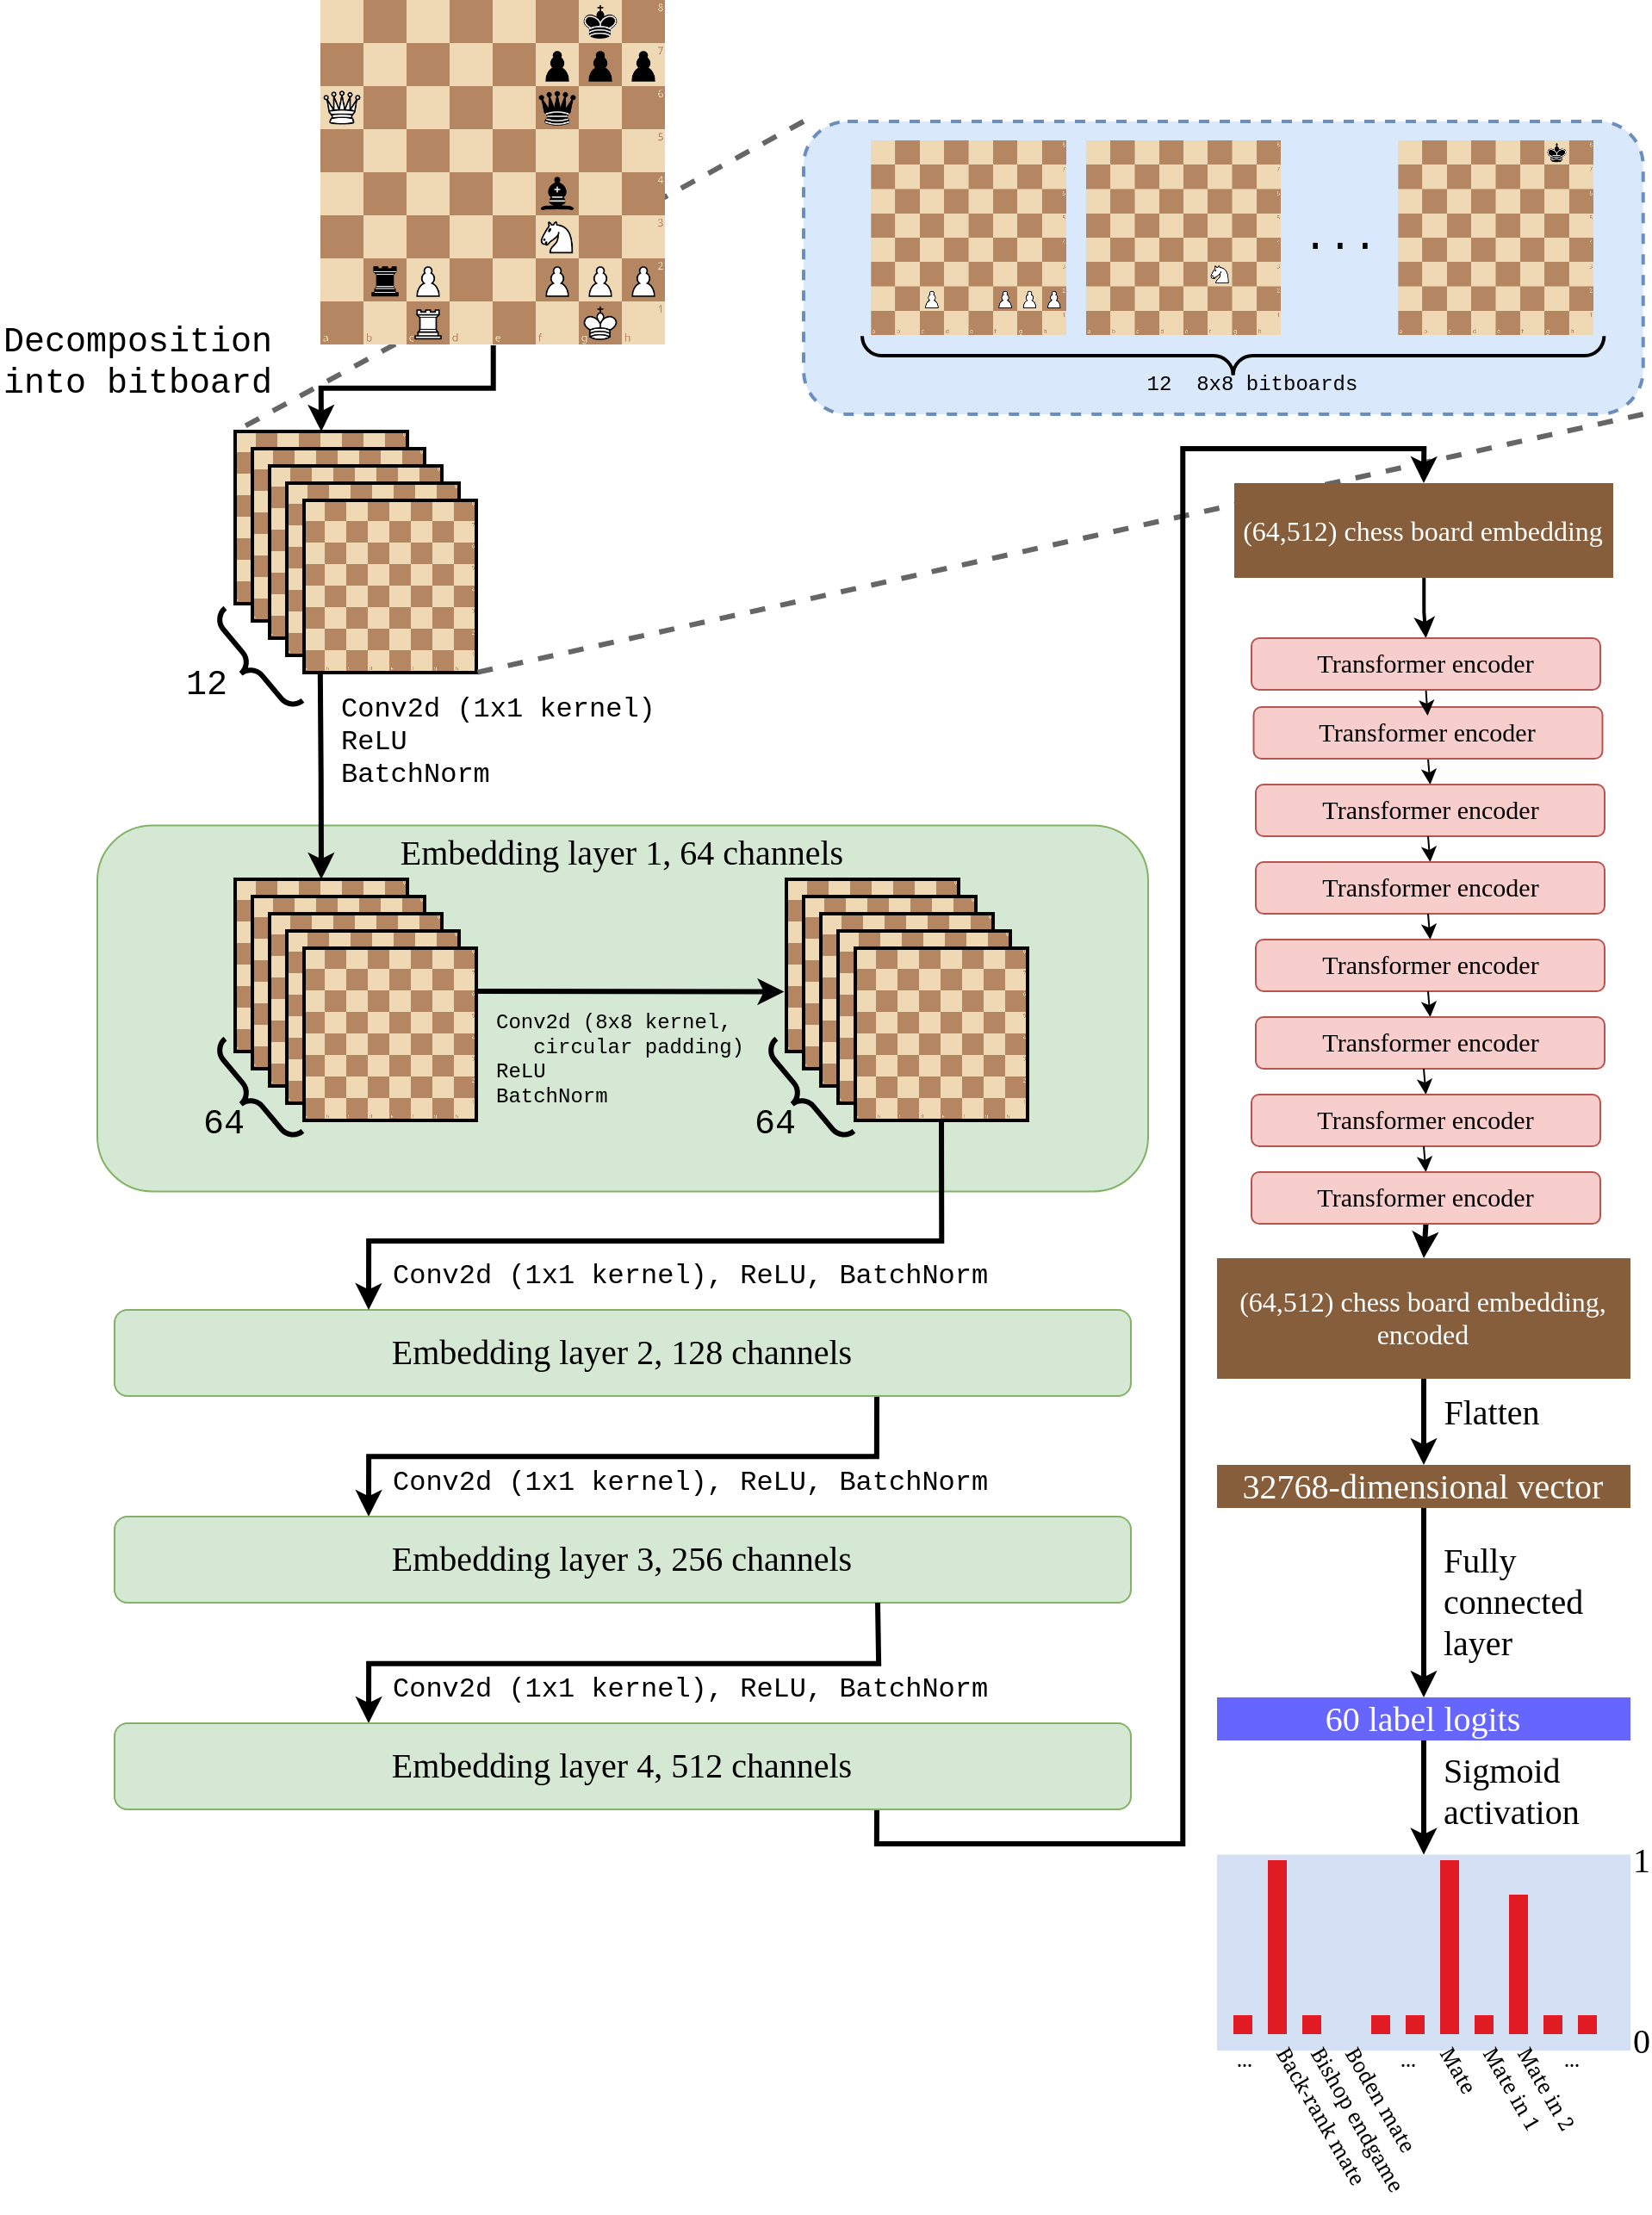
\includegraphics[width=0.65\textwidth]{project/img/ml_diagram.png}
  \caption{High-level overview of the model architecture.}
  \label{MLDiagram}
\end{figure}

\subsection{Training Setup}\label{mlS23}

The model was trained for 5 epochs. The data was batched into batches of size
128, and the average binary cross-entropy loss (\Cref{bceEq}) between the
expected labels and the predicted labels was used as the target to be
minimised. The Adam optimiser \citep{kingma2014adam}, an extension of
stochastic gradient descent, was used for weight updates, with a learning rate
of $1\times10^{-5}$ and default coefficients $\beta_1$, $\beta_2$.

\begin{equation}\label{bceEq}
  L(y, \hat{y}) = -\frac{1}{N}\sum_{i=0}^N \hat{y}_i \log y_i +
    (1-\hat{y}_i)\log(1-y_i)
\end{equation}

The model was trained on the Department of Computing's GPU Slurm Cluster,
managed by \citet{csgGPU}. This cluster contains a multitude of NVIDIA GPUs;
the cited website has an exhaustive list. Each epoch took approximately 1h-2h,
depending on resource availability and hyperparameter combination.

\subsection{Hyperparameters}\label{mlS22}

To find the optimal hyperparameters, a grid search was performed over a subset
of the possible hyperparameter space (\Cref{tabHyperparam}). 

There is evidence of overfitting for the larger models with with $\sim\!33$
million parameters. These achieve a low training loss of approximately 0.08,
but the validation loss greatly suffers as a result. Overall, the
hyperparameter combination with the best performance on the validation set (row
is highlighted) was selected.

The loss curves for this model over the 5 epochs are shown (\Cref{lossCurves}).
While these do not show total convergence, the performance of the model was
adequate. To keep it fair for all combinations, no further training was done
after the search.

\begin{table}[H]
  \centering
  \begin{adjustbox}{width=\textwidth}
    \begin{tabular}{lll|rrr}

      \multicolumn{3}{c}{Hyperparameter} && \multicolumn{2}{c}{Average loss
      after 5 epochs} \\

      Embedding layer channels & \texttt{n\_heads} & \texttt{ff\_dim} & Total
      parameters & Train & Validation\\

      \hline

      $[64, 128, 256, 512 ]$& $32$ & $4096$ & 33,114,812 & 0.08161 & 0.1016   \\
      $[64, 128, 256, 512 ]$& $32$ & $8192$ & 33,114,812 & 0.08156 & 0.1011 \\
      $[64, 128, 256, 512 ]$& $32$ & $16384$ & 33,114,812 & 0.08092 & 0.09937 \\[0.1cm]

      $[64, 128, 256, 512 ]$& $64$ & $4096$ & 33,377,212 & 0.08089 & 0.1026 \\
      $[64, 128, 256, 512 ]$& $64$ & $8192$ & 33,377,212 & \textbf{0.08031} & 0.1019 \\ [0.5cm]

      $[32, 64, 128, 256 ]$& $32$ & $4096$ & 8,846,844 & 0.09416 & 0.09942 \\
      $[32, 64, 128, 256 ]$& $32$ & $8192$ & 8,846,844 & 0.09452 & 0.09991 \\
      $[32, 64, 128, 256 ]$& $32$ & $16384$ & 8,846,844 & 0.09442 & 0.09990 \\[0.1cm]

      $[32, 64, 128, 256 ]$& $64$ & $4096$ & 8,978,172 & 0.09424 & 0.09987 \\
      $[32, 64, 128, 256 ]$& $64$ & $8192$ & 8,978,172 & 0.09395 & 0.09990 \\
      $[32, 64, 128, 256 ]$& $64$ & $16384$ & 8,978,172 & 0.09425 & 0.1001 \\[0.1cm]

      $[32, 64, 128, 256 ]$& $128$ & $4096$ & 9,240,828 & 0.09351 & 0.09918 \\
      $[32, 64, 128, 256 ]$& $128$ & $8192$ & 9,240,828 & 0.09341 & 0.09953 \\
      $[32, 64, 128, 256 ]$& $128$ & $16384$ & 9,240,828 & 0.09387 & 0.09914 \\[0.5cm]

      $[64, 128, 256 ]$& $32$ & $4096$ & 8,779,452 & 0.09234 & 0.09823 \\
      $[64, 128, 256 ]$& $32$ & $8192$ & 8,779,452 & 0.09161 & 0.09787 \\
      $[64, 128, 256 ]$& $32$ & $16384$ & 8,779,452 & 0.09293 & 0.09885 \\[0.1cm]

      $[64, 128, 256 ]$& $64$ & $4096$ & 8,910,780 & 0.09253 & 0.09860 \\
      $[64, 128, 256 ]$& $64$ & $8192$ & 8,910,780 & 0.09288 & 0.09896 \\
      \rowcolor{lightgray} $[64, 128, 256 ]$& $64$ & $16384$ & 8,910,780 & 0.09119 & \textbf{0.09716} \\
     
      $[64, 128, 256 ]$& $128$  & $4096$ & 9,173,436 & 0.09166 & 0.09808 \\
      $[64, 128, 256 ]$& $128$ & $8192$ & 9,173,436 & 0.09154 & 0.09770 \\

    \end{tabular}
  \end{adjustbox}
  \caption{Results of the hyperparameter grid search.}
  \label{tabHyperparam}
\end{table}


\begin{figure}[H]
  \centering
  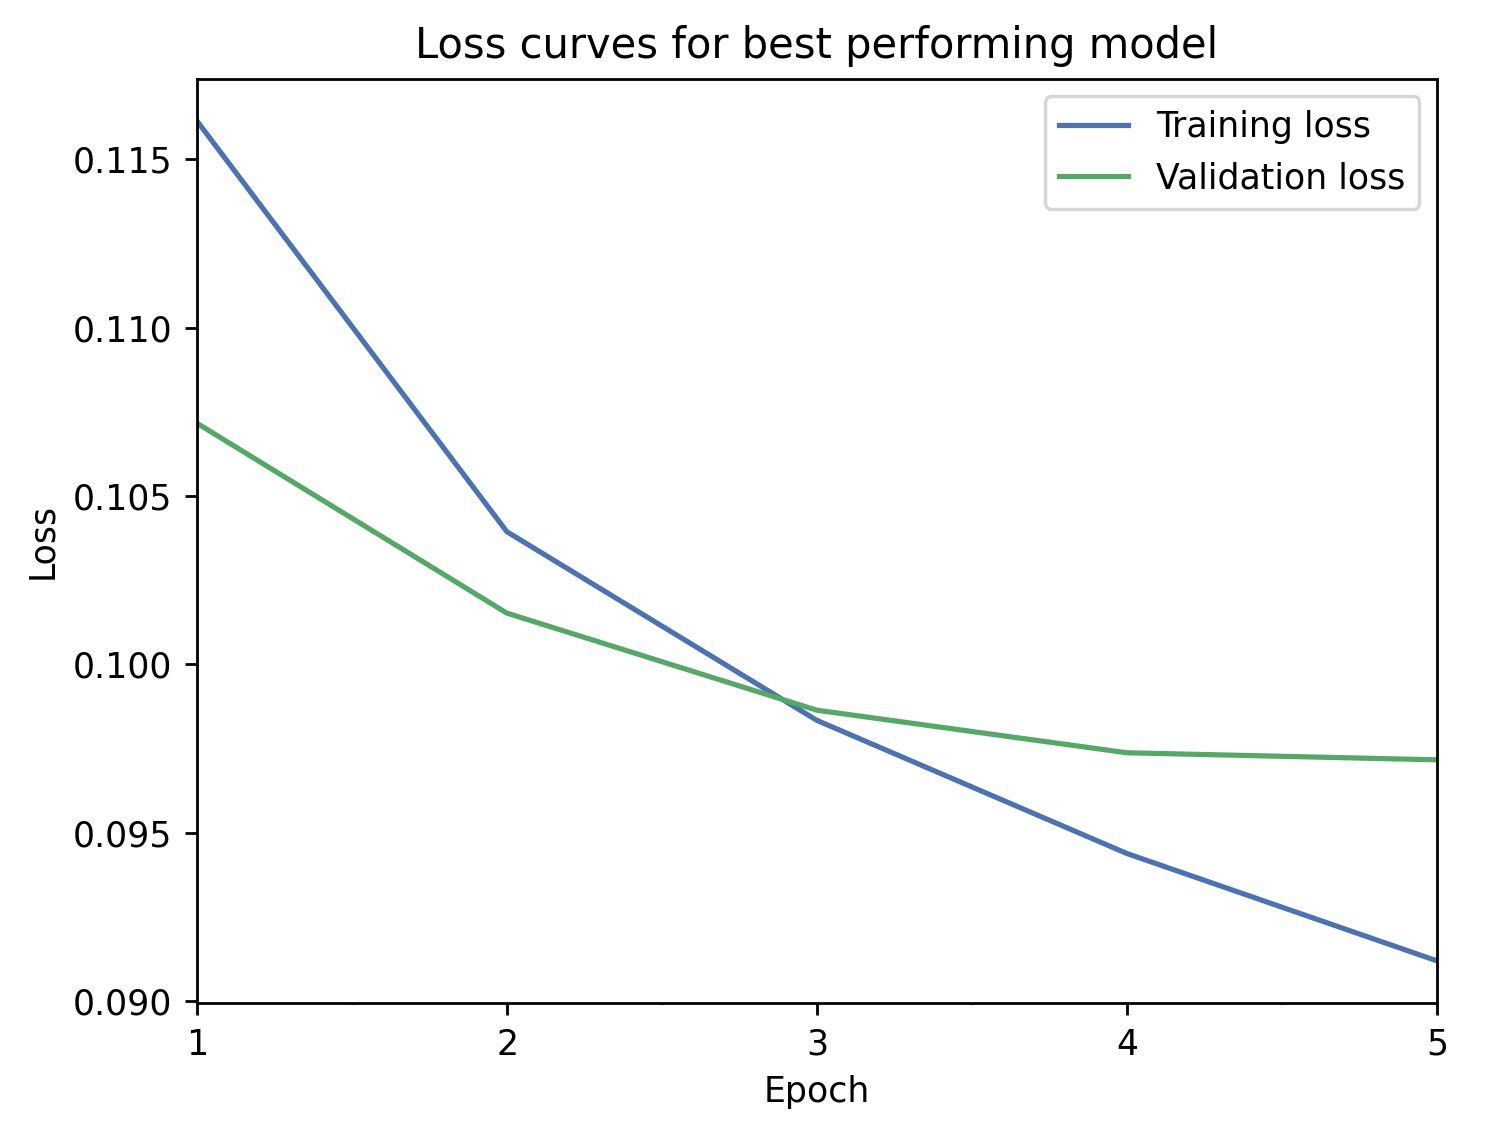
\includegraphics[width=0.5\textwidth]{project/img/loss_curves.png}
  \caption{Training and validation loss of the best performing model.}
  \label{lossCurves}
\end{figure}


\subsection{Conversion to Difficulty Prediction}\label{mlS23}

The architecture, as currently designed, only predicts puzzle themes. In early
experiments, multiple outputs and losses were attempted, but this led to
degradation of performance. To allow the model to predict puzzle difficulty, a
slight modification was made to the architecture (\Cref{mlS21}). 

The 60 output neurons were replaced with just 1: the difficulty rating
prediction. To make learning easier, all difficulties were scaled down by a
factor of 3500. As the difficulty rating range in the dataset is $[399, 3331]$
(\Cref{dataHistogram}), this scaled all ratings to a reasonable range. There
was no activation function for the final neuron.

The loss was changed to mean square error, and no other parameters were
changed. This model was trained with the same hyperparameters as the best
performing label prediction model (\Cref{mlS22}) for 5 epochs. This produced an
entirely new model.

\section{Visualisations of the Model}\label{mlS3}

Previously, the idea of chess pieces and squares interacting with each other
was shown (\Cref{chessPuzzleLinks}). With a trained model, this can now be
explored further. As the bitboards flow through the model, attention values and
weights can be extracted from each transformer encoder layer. By unflattening
them back into a $8\times8$ chess board, interesting patterns are seen.

\subsection{Interpretation}

Attention values and weights are shown below for the puzzle which was used to
illustrate how transformers could work in this problem
(\Cref{chessPuzzleLinks}). The values diagram (\Cref{atnZ}) shows each channel
of the chess board at that stage in the model. In the case of this model, there
are 256 channels, each of size $8\times8$. 

The weights diagram (\Cref{atnZ1}) shows the weights of the self-attention
within the transformer architecture. This diagram has 64 heatmaps, arranged in
a chess board-like arrangement. Each heatmap represents the weights it assigns
to the other board locations when updating its own embedding in the
self-attention stage.

To see a concrete example, take the top left heatmap, corresponding to the
\texttt{a8} square. This value assigns a very positive weight to the
\texttt{g8} square (yellow dot in the top right), and a much lower (possibly
negative) weight to the middle ranks in the board.


\begin{figure}[H]
  \begin{minipage}{0.475\textwidth}
    \centering
    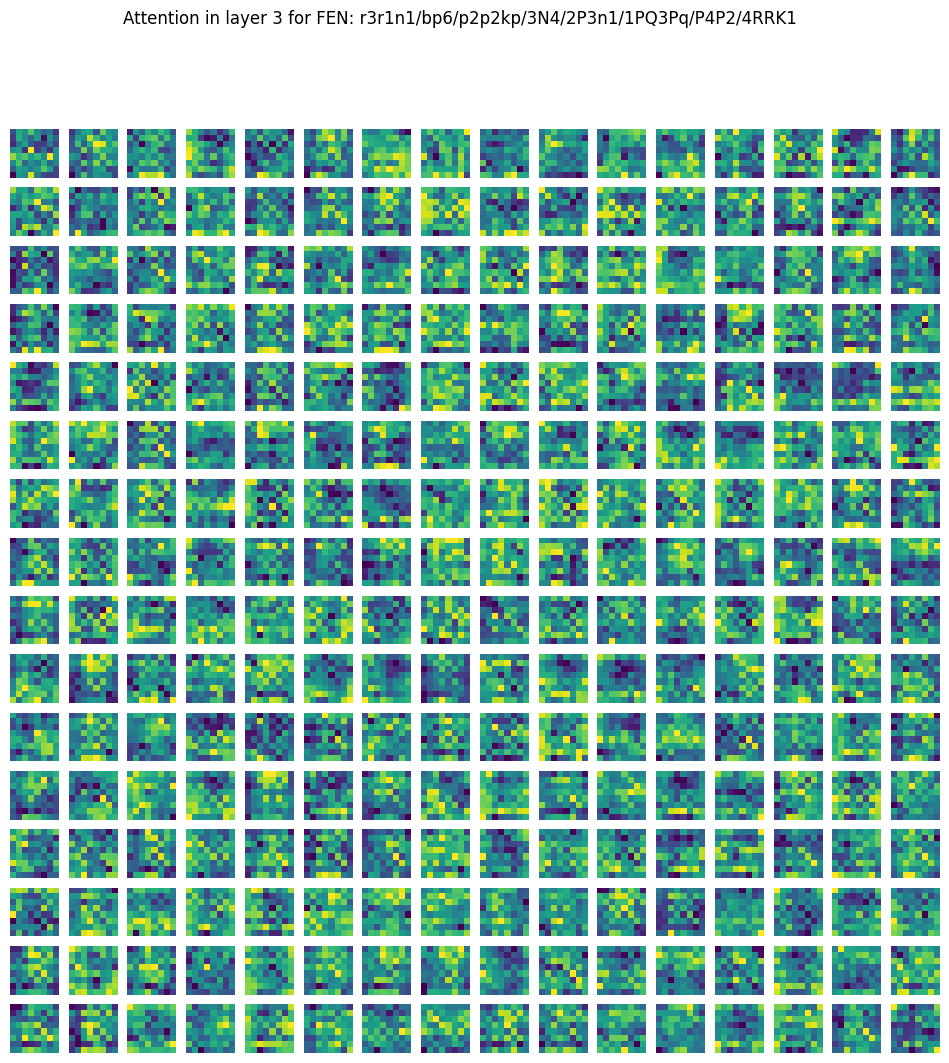
\includegraphics[width=\textwidth]{project/img/attention_maps/attention_3.png}
    \caption{Chess puzzle attention values in layer 3 of the transformer encoder.}
    \label{atnZ}
  \end{minipage}
  \hspace{0.05\textwidth}
  \begin{minipage}{0.475\textwidth}
    \centering
    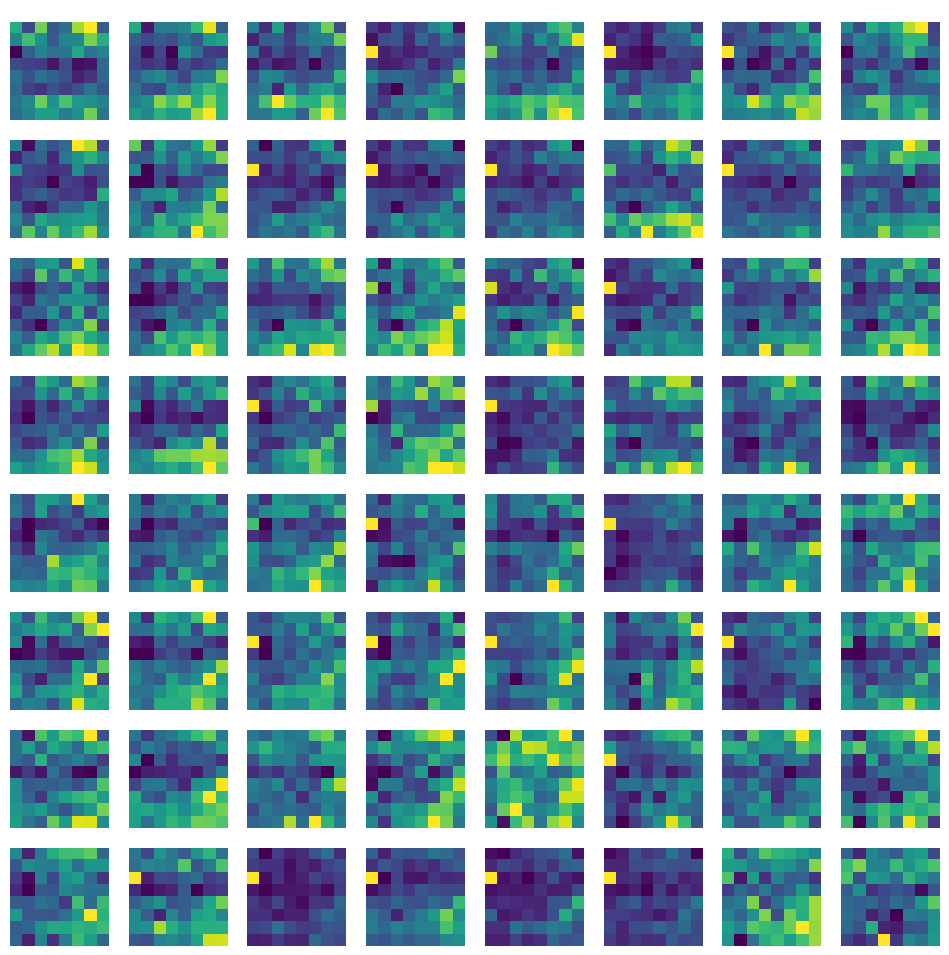
\includegraphics[width=\textwidth]{project/img/attention_maps/weights_4.png}
    \caption{Chess puzzle attention weights in layer 4 of the transformer encoder.}
    \label{atnZ1}
  \end{minipage}
\end{figure}

\subsection{Attention Weights and Values of Single Chess Pieces}\label{mlS32}

In this section, a single chess piece is placed on \texttt{e4} and this
position is passed through the model. The corresponding attention value and
weight heatmaps are shown.

\paragraph{Rook} Horizontal and vertical patterns can be seen in both diagrams.
This, of course, stems from the moveset of the rook.

\begin{figure}[H]
  \begin{minipage}{0.475\textwidth}
    \centering
    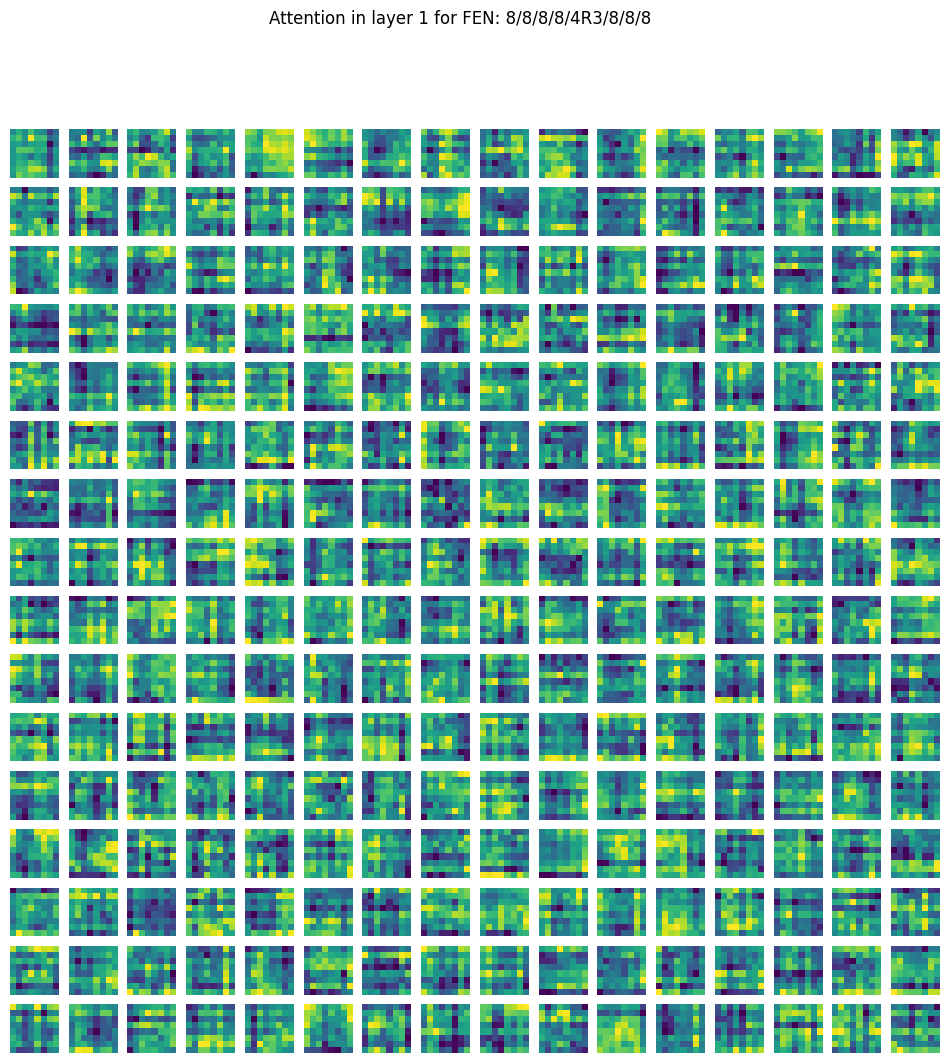
\includegraphics[width=\textwidth]{project/img/attention_maps/R_attention_1.png}
    \caption{Rook attention values.}
    \label{atnR1}
  \end{minipage}
  \hspace{0.05\textwidth}
  \begin{minipage}{0.475\textwidth}
    \centering
    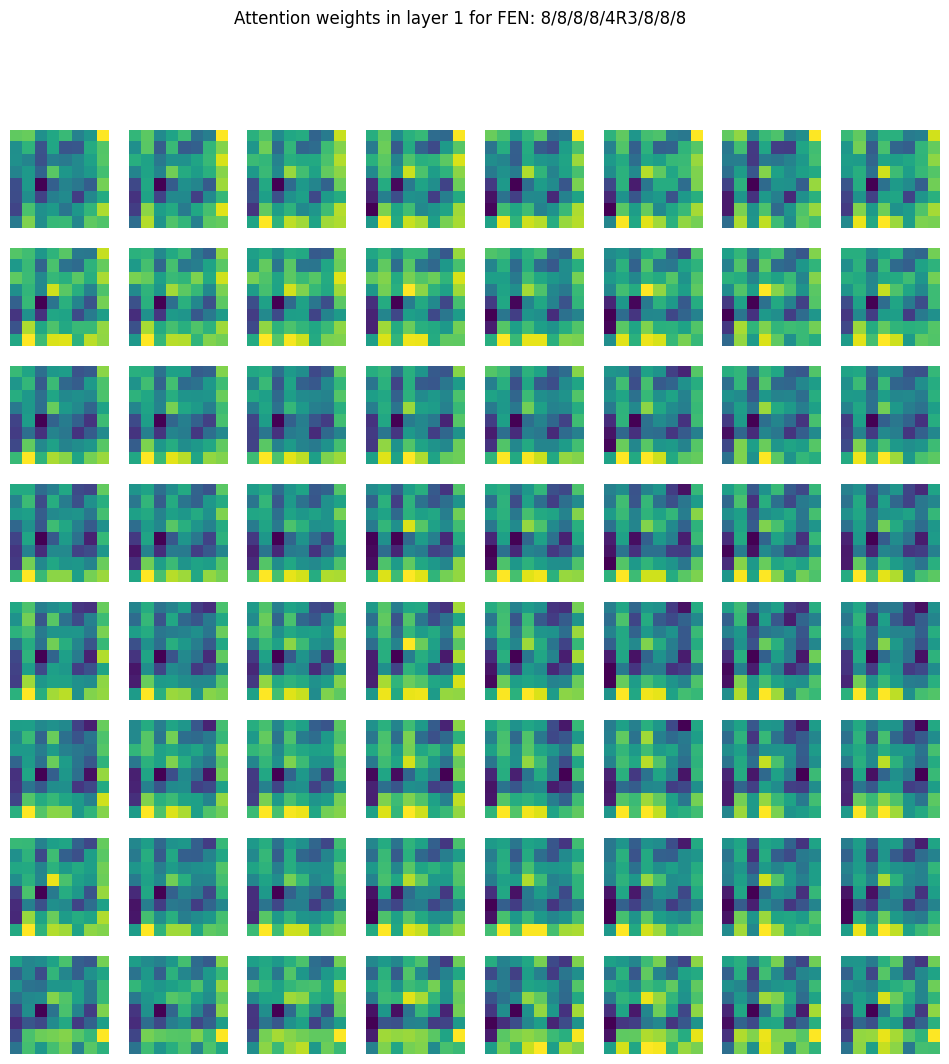
\includegraphics[width=\textwidth]{project/img/attention_maps/R_weights_1.png}
    \caption{Rook attention weights.}
    \label{atnR}
  \end{minipage}
\end{figure}

\newpage

\paragraph{Bishop} This bishop is a light-squared bishop. Bishops can only move
diagonally, and this means that half of the board will never be accessible to
the bishop, which explains the checkerboard nature of the heatmaps.
Interestingly, the weights diagram (\Cref{atnB1}) shows how important the main
diagonal is, which is controlled by the bishop. Every other square takes it
into consideration when updating its own value.

\begin{figure}[H]
  \begin{minipage}{0.475\textwidth}
    \centering
    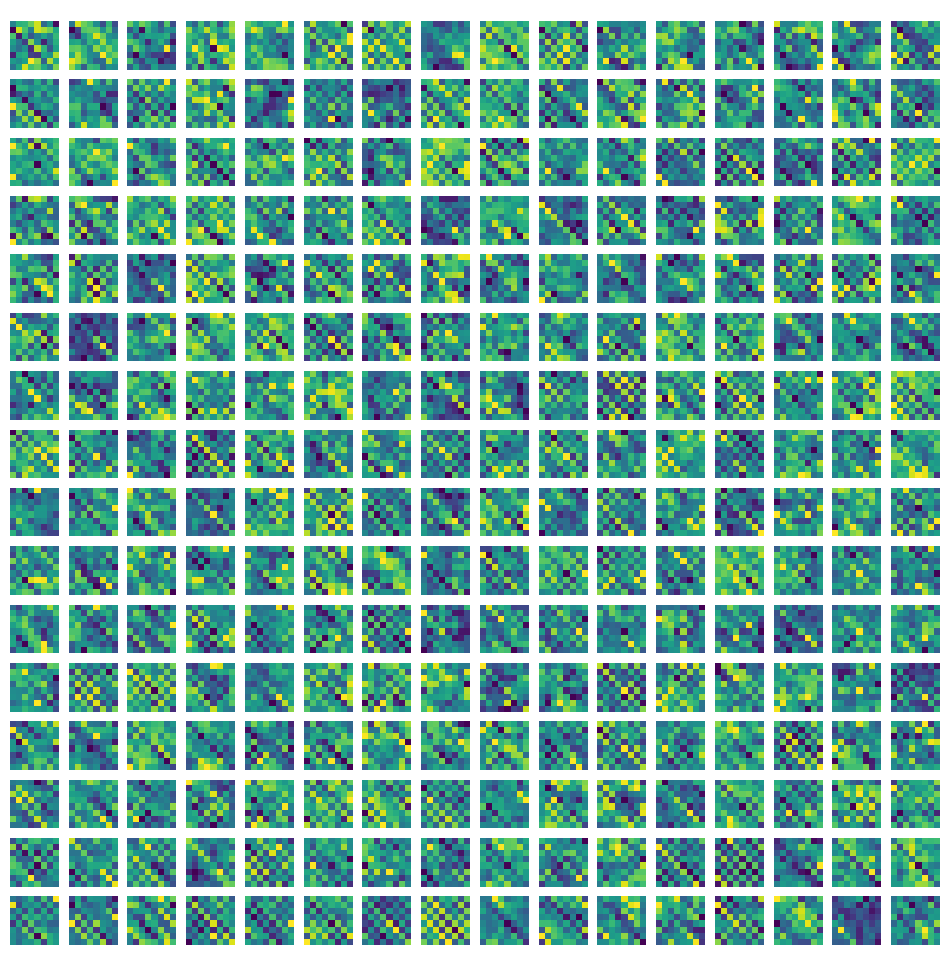
\includegraphics[width=\textwidth]{project/img/attention_maps/B_attention_4.png}
    \caption{Bishop attention values.}
    \label{atnB}
  \end{minipage}
  \hspace{0.05\textwidth}
  \begin{minipage}{0.475\textwidth}
    \centering
    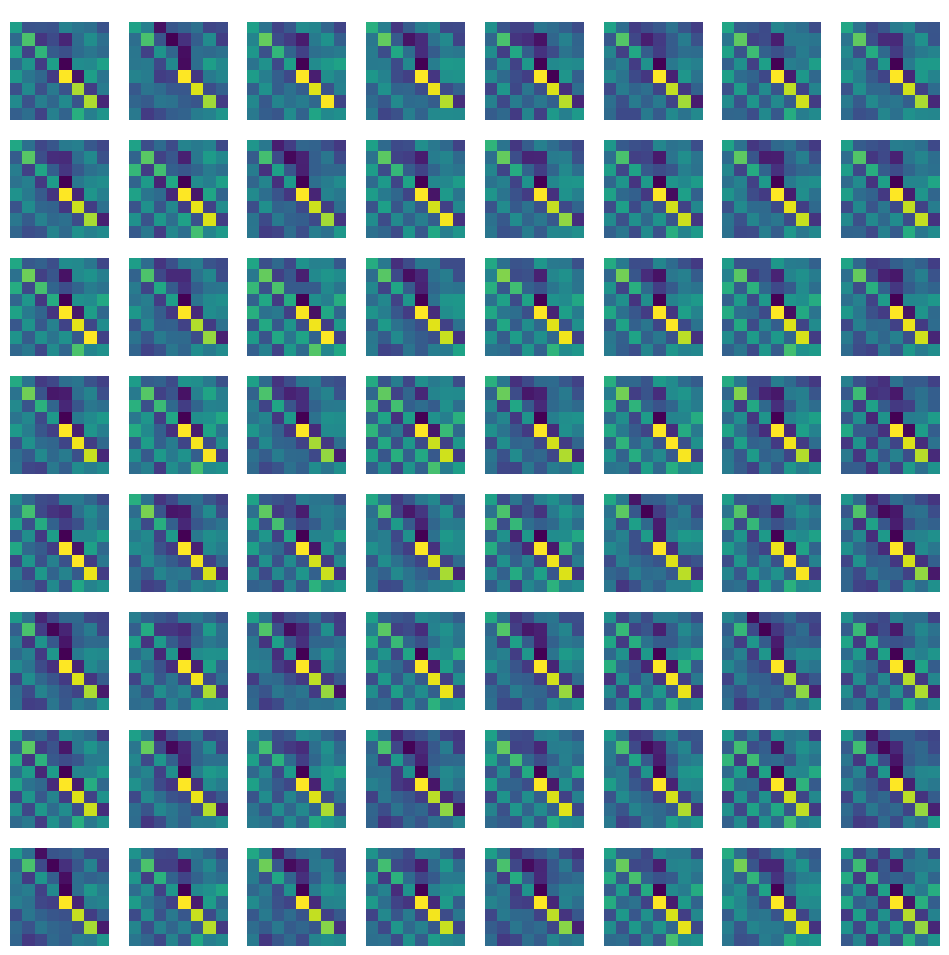
\includegraphics[width=\textwidth]{project/img/attention_maps/B_weights_4.png}
    \caption{Bishop attention weights.}
    \label{atnB1}
  \end{minipage}
\end{figure}

\paragraph{Queen} The queen combines the moveset of the rook and bishop, and
this can be seen in the heatmaps, as they are less structured. The weights
heatmap shows that the \texttt{h7} square is important -- this is possibly
because many checkmates are delivered by the queen on this square, and the
queen has vision of \texttt{h7} from \texttt{e4}.

\begin{figure}[H]
  \begin{minipage}{0.475\textwidth}
    \centering
    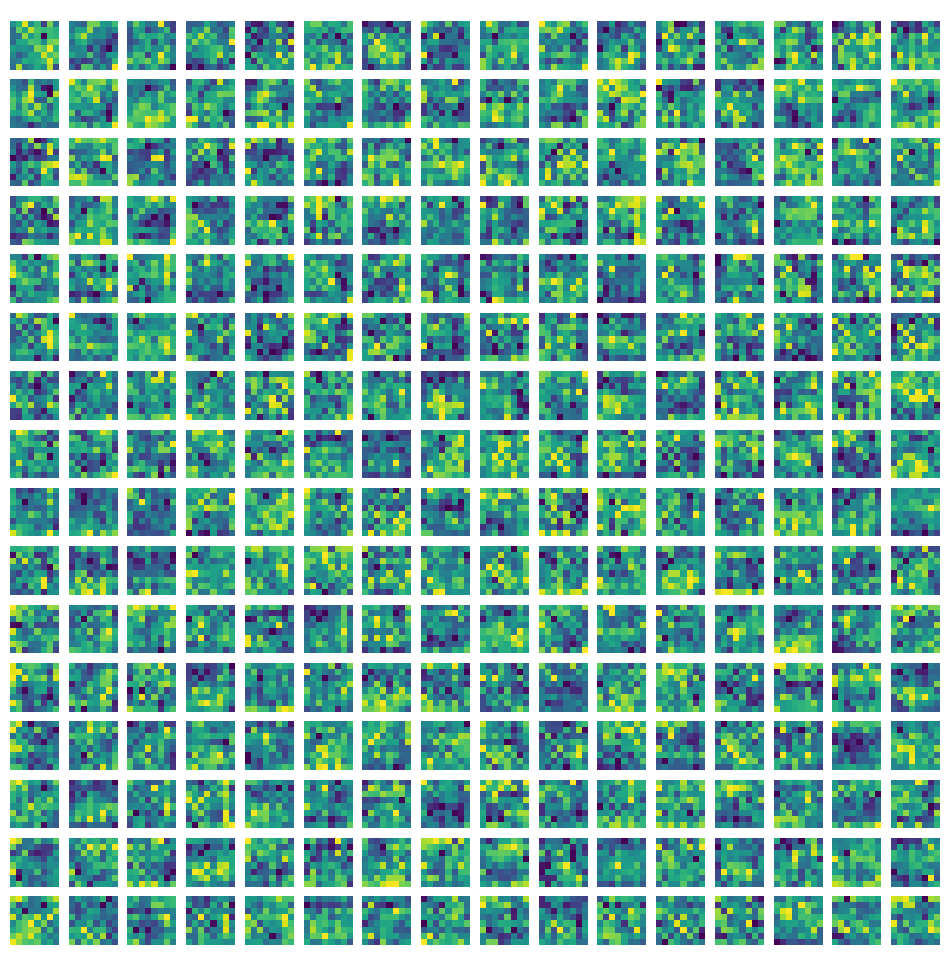
\includegraphics[width=\textwidth]{project/img/attention_maps/Q_attention_6.png}
    \caption{Queen attention values.}
    \label{atnQ}
  \end{minipage}
  \hspace{0.05\textwidth}
  \begin{minipage}{0.475\textwidth}
    \centering
    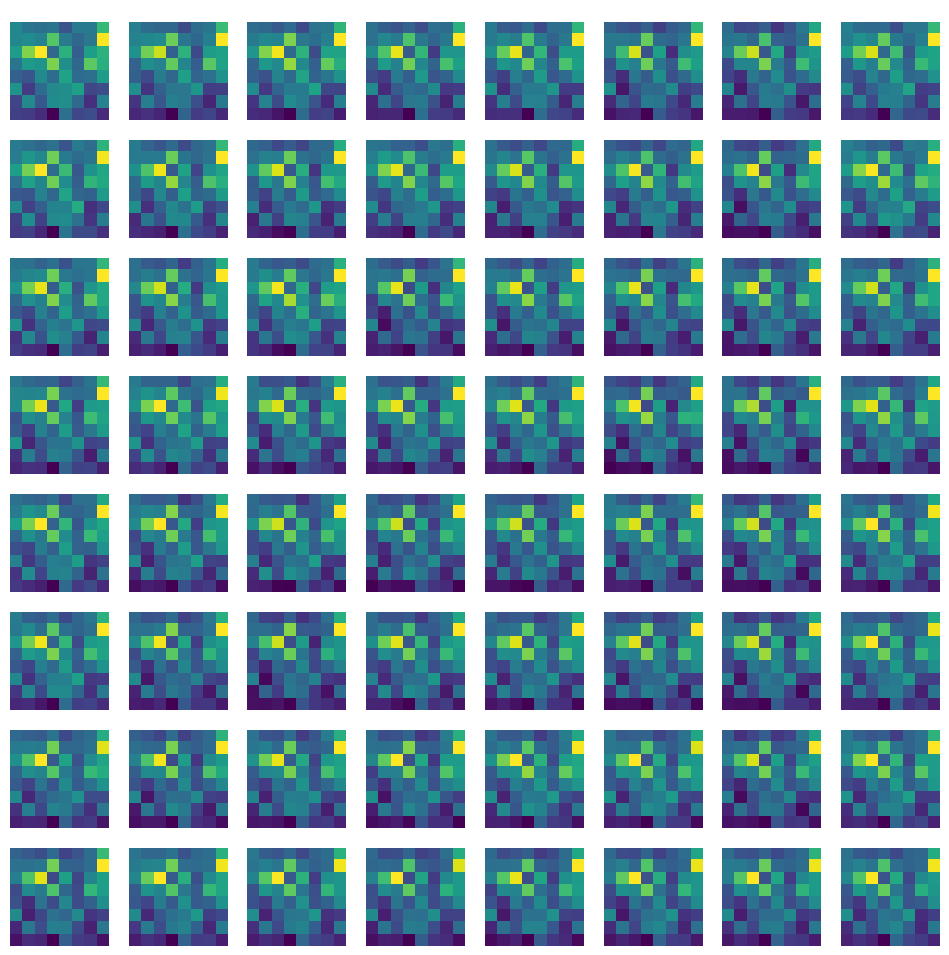
\includegraphics[width=\textwidth]{project/img/attention_maps/Q_weights_6.png}
    \caption{Queen attention weights.}
    \label{atnQ1}
  \end{minipage}
\end{figure}

\newpage

\paragraph{Knight} The knight heatmaps have a checkerboard pattern similar to
the bishop's. This is likely a result of its moveset: a knight attacks
squares of the opposite colour to the square it is on.

\begin{figure}[H]
  \begin{minipage}{0.475\textwidth}
    \centering
    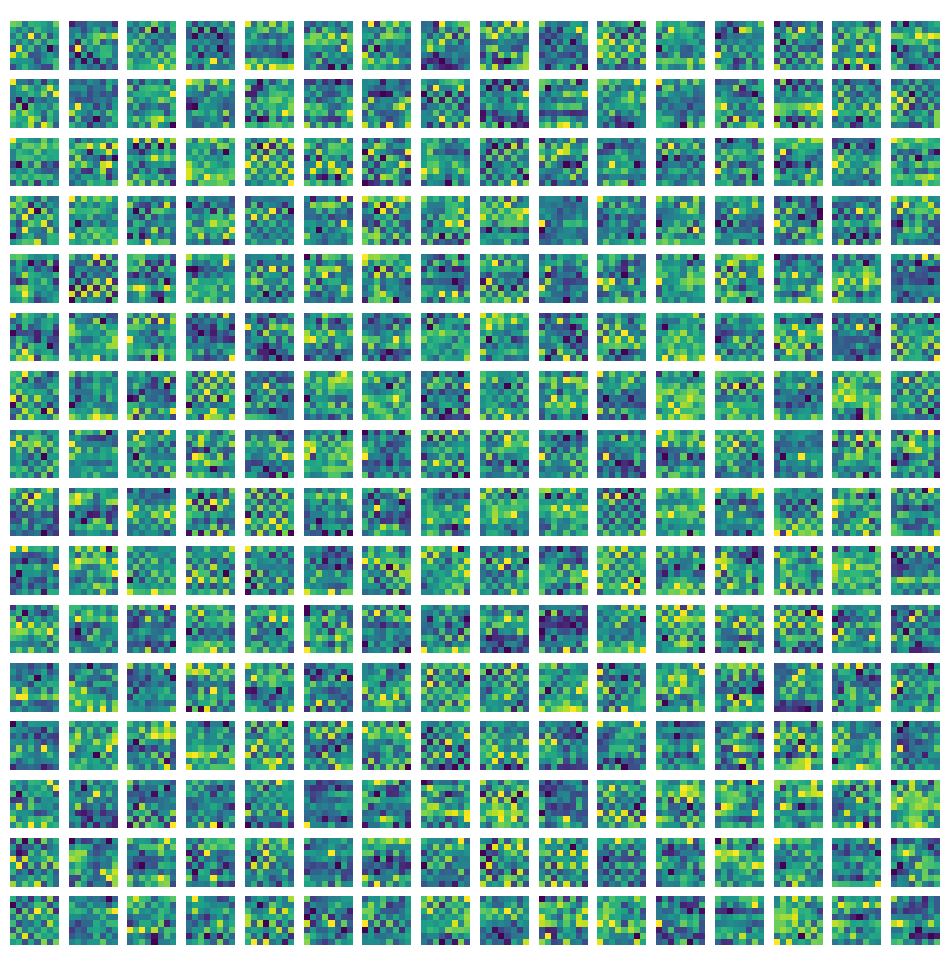
\includegraphics[width=\textwidth]{project/img/attention_maps/N_attention_1.png}
    \caption{Knight attention values.}
    \label{atnN}
  \end{minipage}
  \hspace{0.05\textwidth}
  \begin{minipage}{0.475\textwidth}
    \centering
    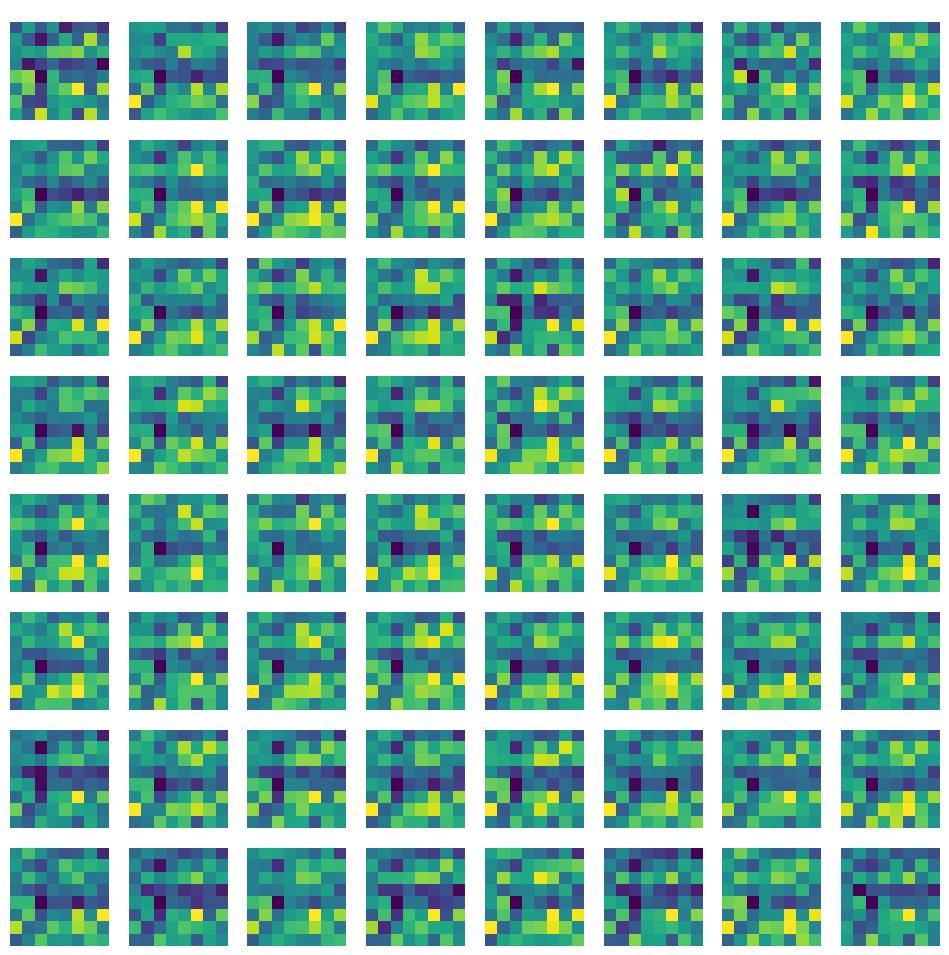
\includegraphics[width=\textwidth]{project/img/attention_maps/N_weights_1.png}
    \caption{Knight attention weights.}
    \label{atnN1}
  \end{minipage}
\end{figure}


\paragraph{Pawn} Pawns can only move forwards and usually come in groups,
aligned horizontally. This is clearly seen in both of the attention heatmaps.
The weights heatmap (\Cref{atnP1}) especially highlights this: the files in
front of the pawn and behind the pawn are important, as these usually have
pawns supported by, or supporting the \texttt{e4} pawn.

\begin{figure}[H]
  \begin{minipage}{0.475\textwidth}
    \centering
    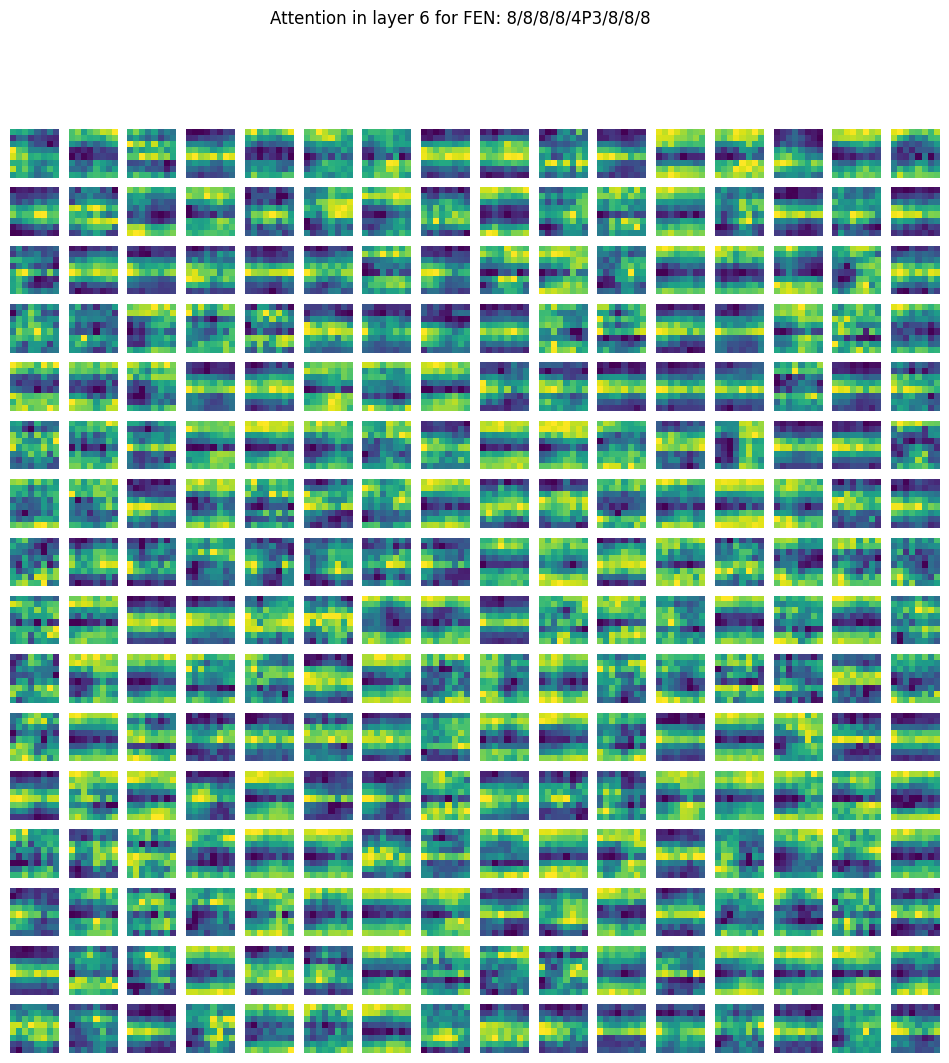
\includegraphics[width=\textwidth]{project/img/attention_maps/P_attention_6.png}
    \caption{Pawn attention values.}
    \label{atnP}
  \end{minipage}
  \hspace{0.05\textwidth}
  \begin{minipage}{0.475\textwidth}
    \centering
    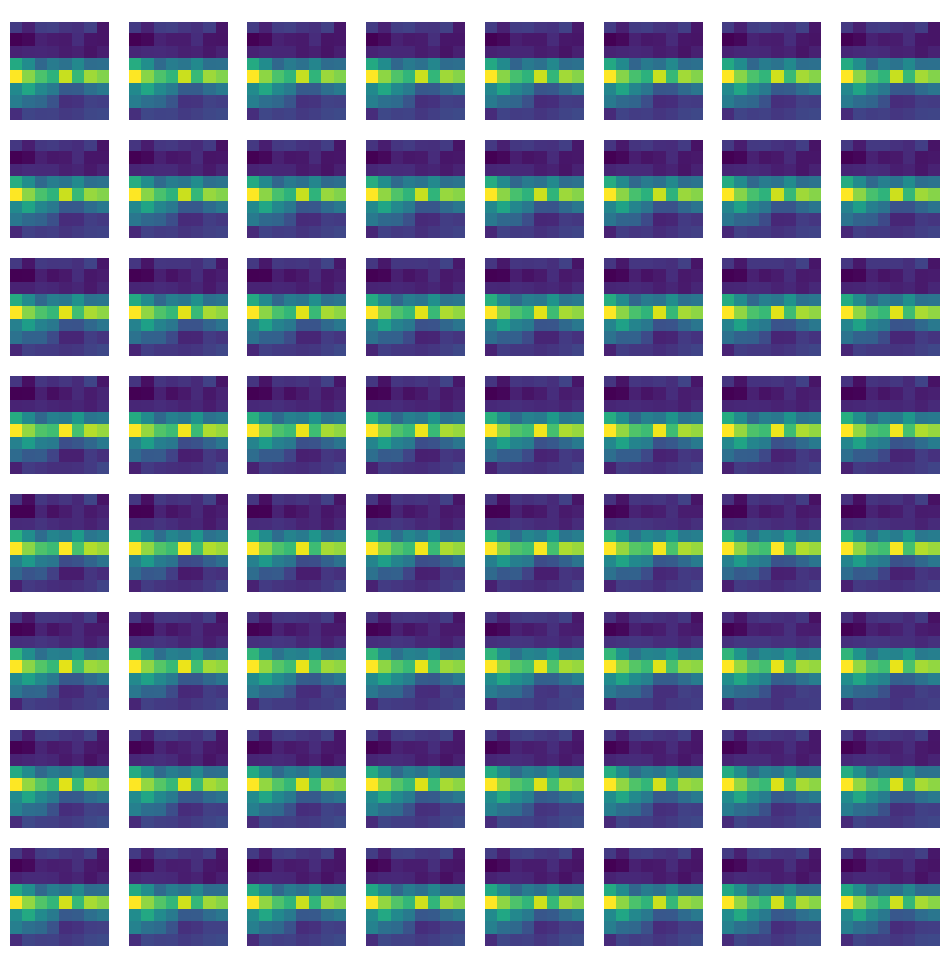
\includegraphics[width=\textwidth]{project/img/attention_maps/P_weights_6.png}
    \caption{Pawn attention weights.}
    \label{atnP1}
  \end{minipage}
\end{figure}

\newpage

\paragraph{King} Finally, the king. The attention weights heatmap
(\Cref{atnK1}) shows heavy importance of the \nth{1} and \nth{8} files -- where
the kings are usually located.


\begin{figure}[H]
  \begin{minipage}{0.475\textwidth}
    \centering
    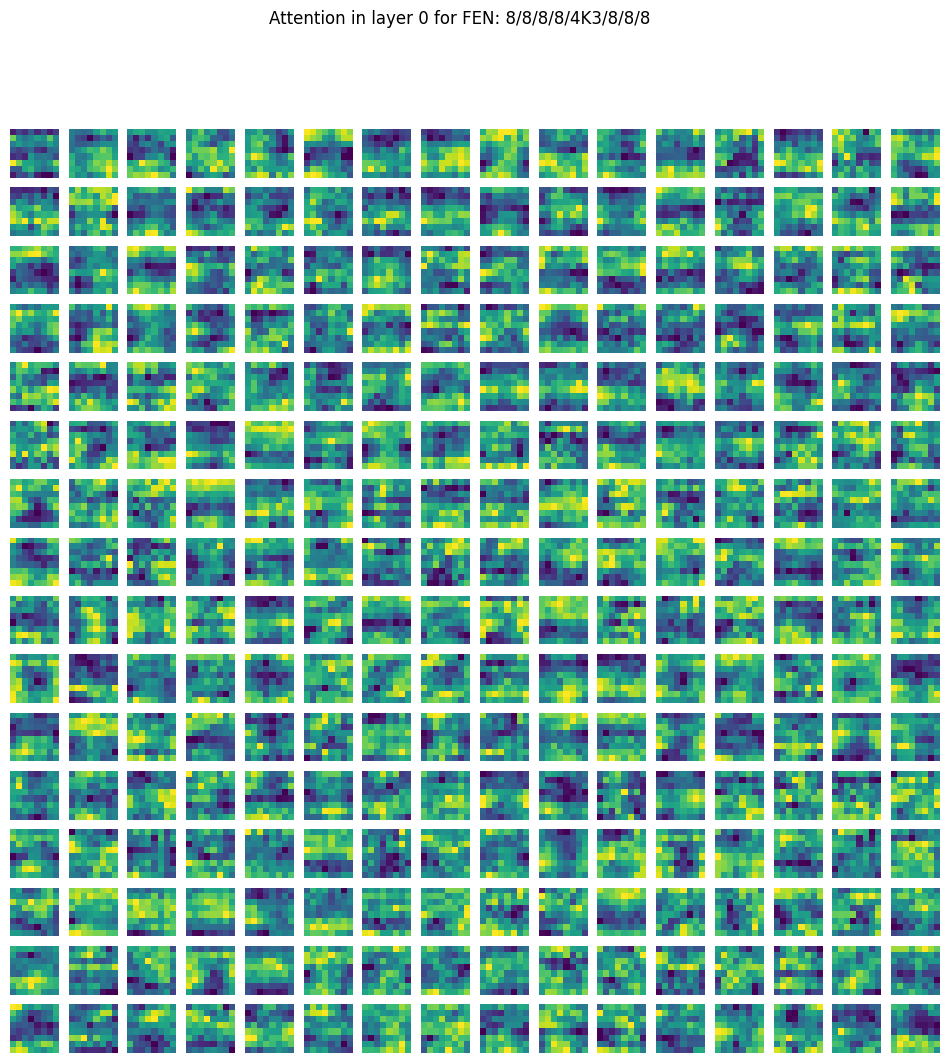
\includegraphics[width=\textwidth]{project/img/attention_maps/K_attention_0.png}
    \caption{King attention values.}
    \label{atnK}
  \end{minipage}
  \hspace{0.05\textwidth}
  \begin{minipage}{0.475\textwidth}
    \centering
    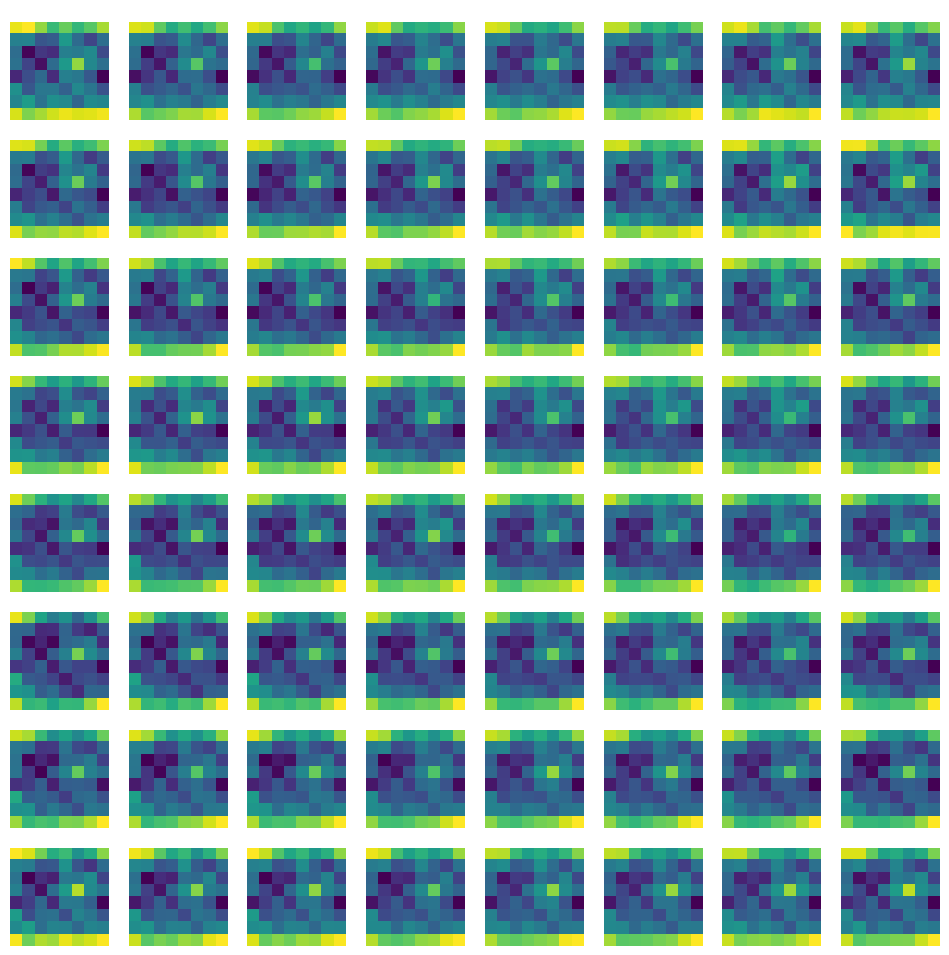
\includegraphics[width=\textwidth]{project/img/attention_maps/K_weights_0.png}
    \caption{King attention weights.}
    \label{atnK1}
  \end{minipage}
\end{figure}

\subsection{Discussion}\label{mlS33}

The patterns generated by the model (\Cref{mlS32}) are incredible, given the
model has zero information about the game of chess other than a collection of
static positions and labels. This is reminiscent of the work of
\citet{chess2vec} (\Cref{bg4}), who were able to find success without
explicitly implementing chess logic.

This shows that transformers have untapped potential in the area of chess, as
these patterns were learned in order to label puzzles effectively. Playing
chess, which would require a deeper understanding of piece interactions and
positions, was not a target, and despite this, progress towards it seems to
have been made.




\chapter{The Tree-Based Approach}\label{treeChapter}

In this chapter, a different novel approach to puzzle classification is
proposed, focusing on the applications of a custom distance function defined
between chess puzzles' meaningful search trees.

Initially, the concept of labelled search trees and distance is introduced
(\Cref{treeS1}). This includes a high-level description of how to create these
trees (\Cref{treeS12,treeS13}) and how to measure distance between them
(\Cref{treeS21}).

Unsupervised clustering (\Cref{treeS2}) naturally follows these concepts. The
results of this are shown (\Cref{treeS22}), along with concrete examples and
visualisations (\Cref{treeS23}).

Afterwards, $k$-Nearest Neighbours (\Cref{treeS3}) is used for the downstream
task of puzzle label and difficulty rating prediction. Its performance is
evaluated and compared to the deep learning approach (\Cref{mlChapter}) in the
next chapter.

\section{Overview}\label{treeS1}

This method seeks to combine and build upon two approaches seen in the above
literature review: the tree-based puzzle difficulty classification by
\citet{chessTrees} and chess position similarity using dynamic features by
\citet{chessMotifs} (\Cref{typeAndDifficultyReview}).

By combining these approaches to construct meaningful search trees with
additional node labels, defining a distance function for individual chess
moves, and applying a labelled tree edit distance function
\citep{editDistTrees}, it will be possible to calculate `closeness' of chess
puzzles. 

\subsection{Representing Puzzles With Labelled Trees}\label{treeS11}

As explored by \citet{chessTrees}, `meaningful search trees' have predictive
ability of a puzzle's difficulty. These trees are constructed by analysing
powerful moves that either gain, or at least do not worsen a side's position. 

This work can be built upon by additionally labelling these trees with move
information. To build the intuition behind this idea, there are two labelled
search trees (\Cref{tree3,tree4}) of visually distinct, but tactically
identical chess positions (\Cref{puzzle5,puzzle6}), which were found by the
work of \citet{chessMotifs}.

In these trees, algebratic notation of the moves is shown, along with 4
slash-delimited integers, which correspond to: pieces attacked, pieces
defended, number of attackers, number of defenders.\footnote{As the moves must
be legal, this means a king move will never have any attackers, and any
check/mate will have at least 1 piece attacked: the enemy king.} Both of these
chess puzzles feature a \emph{rook sacrifice}, and an imminent queen checkmate
helped by the powerful light-squared bishop. This similarity is not immediately
obvious, but the search trees for these puzzles are almost identical, except for
minor attacker/defender discrepancies. These puzzles were already successfully
grouped by \citet{chessMotifs}.

More complicated positions (\Cref{chess5,chess6}) naturally have more
complicated move trees. Despite being visually distinct, these positions are also
tactically similar. They were found by \citet{chessLanguage} (\Cref{concWork}).
While the 2 trees do not look similar visually (their size being the main
problem), the first 3 halfmoves are almost identical. 

\begin{figure}[H]
  \begin{minipage}[t]{0.475\textwidth}
    \centering
    \chessboard[setfen= 4r1k1/1b3pp1/4p3/p2r4/7R/2B1Q1PP/P1P1RP1K/1q6 w - -
    0 1]
    \caption{Taken from `Automatic Recognition of Similar Chess Motifs' by
    \citet{chessMotifs}. White mates in three moves (\texttt{1.Rh8+ Kxh8 2.Qh6+
    Kg8 3.Qxg7#}).}
    \label{puzzle5}
  \end{minipage}
  \hspace{0.05\textwidth}
  \begin{minipage}[t]{0.475\textwidth}
    \centering
    \chessboard[setfen=r5k1/5pp1/8/3p3R/2q4P/PbB2P2/1P1Q2P1/K7 w q - 0 1]
    \caption{Also taken from `Automatic Recognition of Similar Chess Motifs' by
    \citet{chessMotifs}. White mates in three with the same moves as the puzzle
    on the left.}
    \label{puzzle6}
  \end{minipage}
\end{figure}

\begin{figure}[H]
  \begin{minipage}{0.475\textwidth}
    \centering
    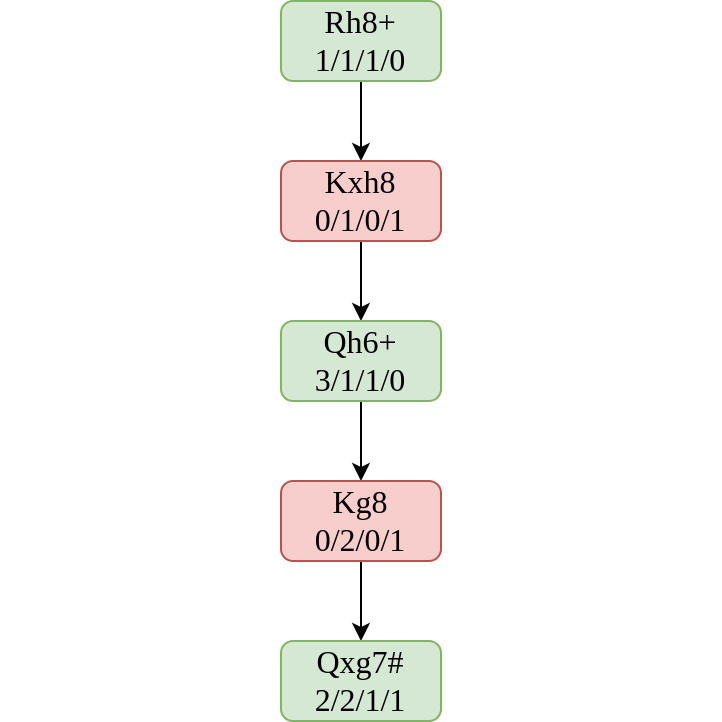
\includegraphics[width=\textwidth]{project/img/trees/3.drawio.png}
    \caption{Labelled search tree for the game above (\Cref{puzzle5}).}
    \label{tree3}
  \end{minipage}
  \hspace{0.05\textwidth}
  \begin{minipage}{0.475\textwidth}
    \centering
    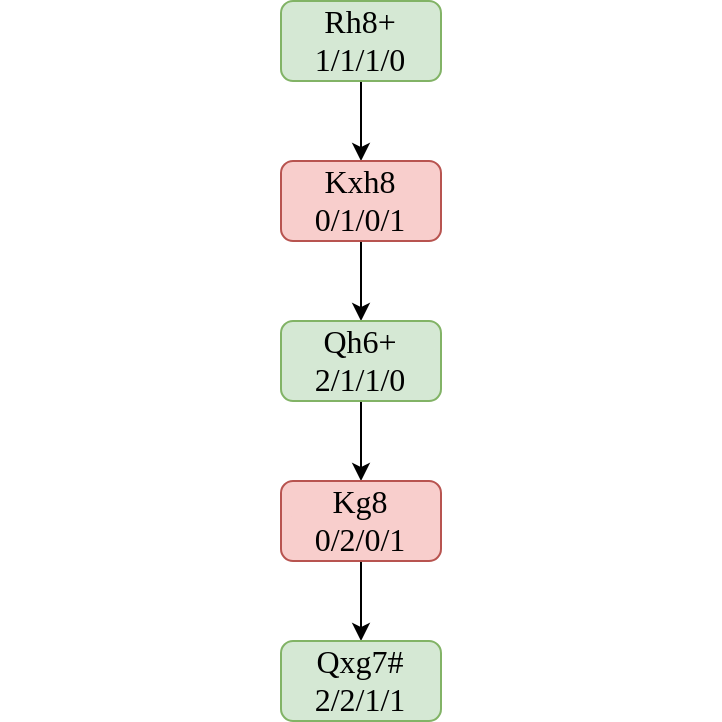
\includegraphics[width=\textwidth]{project/img/trees/4.drawio.png}
    \caption{Labelled search tree for the game above (\Cref{puzzle6}).}
    \label{tree4}
  \end{minipage}
\end{figure}

\begin{figure}[H]
  \begin{minipage}{0.475\textwidth}
    \centering
    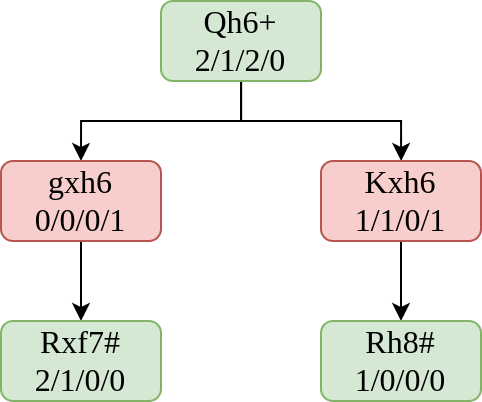
\includegraphics[width=\textwidth]{project/img/trees/1.drawio.png}
    \caption{Labelled search tree for game in \Cref{chess5}}
    \label{tree1}
  \end{minipage}
  \hspace{0.05\textwidth}
  \begin{minipage}{0.475\textwidth}
    \centering
    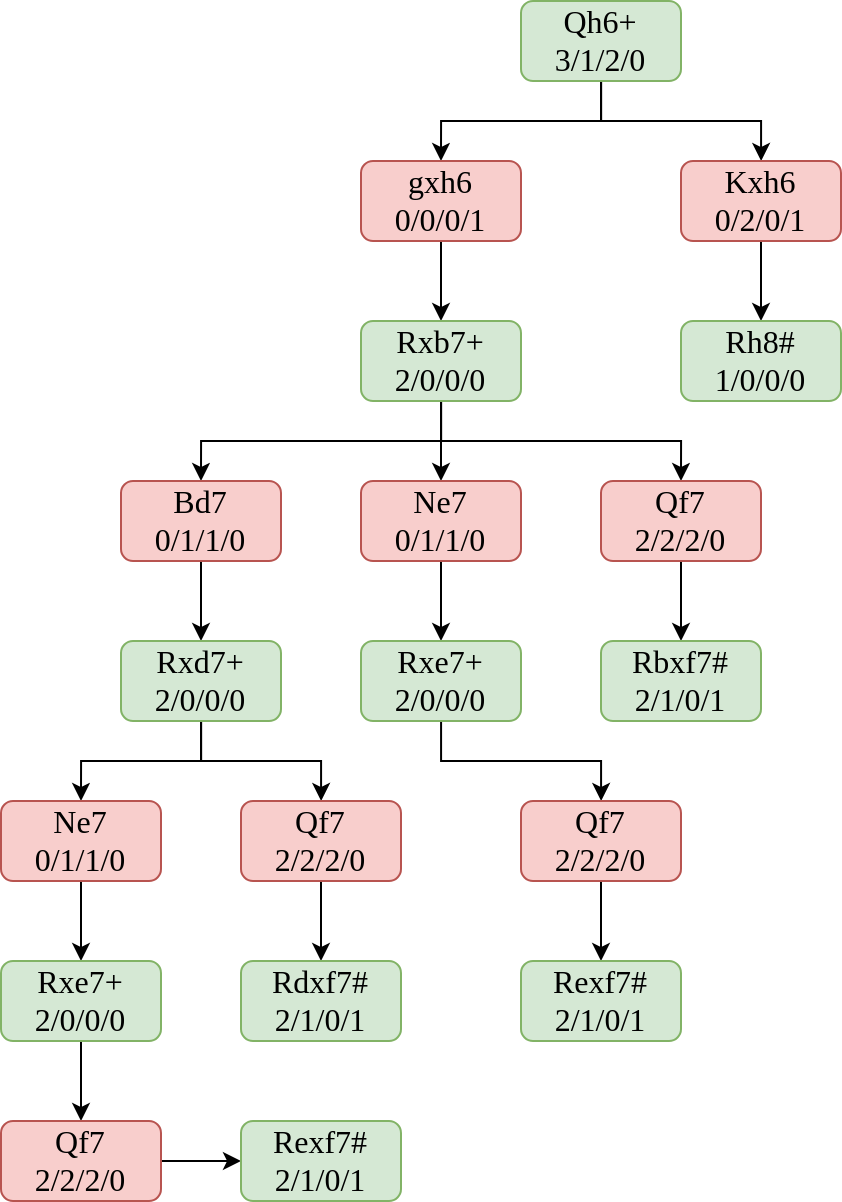
\includegraphics[width=\textwidth]{project/img/trees/2.drawio.png}
    \caption{Labelled search tree for game in \Cref{chess6}}
    \label{tree2}
  \end{minipage}
\end{figure}

\subsection{Meaningful Tree Generation}\label{treeS12}

Similar to the work of \citet{chessTrees}, Stockfish (depth=20) was used to
generate meaningful trees of a maximum depth of 5 halfmoves. Each level of the
tree has a maximum of 4 possible moves that are within 100 centipawns
(arbitrarily chosen) of the best move. To simplify analysis, all puzzles are
transformed to be from White's perspective.

\citet{chessTrees} writes: ``[A high branching factor] means that the position
is already so strong that it no longer matters what move the player chooses
because almost everything wins.''; the tree search is terminated if the best 4
moves for the losing side are within 100 centipawns. While this differs from
the quote above, it causes trees to terminate when the puzzle is completed (any
move for the losing side is equally bad), as opposed to one move before (any
move for the winning side is equally good). Finally, a checkmate naturally
indicates that the puzzle is solved. 

This analysis is continued until either every branch of the puzzle is
exhausted. This happens because it either has solved the puzzle, or reached the
maximum depth.

Whilst generating the tree nodes, each move is annotated with a list of
attributes describing the properties of these move, such as the name of the
piece, whether it delivers check, and how many pieces it is defended by.

In total, 3.8 million game trees were generated, which took about 10,000 hours
of CPU time. This was done with the help of the Department of Computing's
HTCondor cluster, managed by \citet{csgCondor}.

\subsection{What Makes Chess Moves Similar?}\label{treeS13}

To compare arbitrary tree nodes, a distance function was created -- this can be
used in the tree edit algorithm to find the distance between trees. The
properties of the moves in each node are compared, and any difference incurs a
penalty (\Cref{distanceTable}). These penalties are completely arbitrary and
were chosen by an intermediate chess player.

The penalty for adding or removing a node was set to 250. The final distance
between the node is given by the sum of all the individual penalties,
multiplied by a `depth multiplier'. These multipliers heavily discourage puzzle
difference at the beginning of the solution, and allow greater differences
towards the end. In early experiments, it was found that puzzles may have a
similar tactic at the beginning, which is crucial to their similarity, and a
different ending, which is less important. The depth multipliers are: $4, 1,
0.5, 0.25, 0.1, 0.05$ for depths $0$ through to $5$, respectively.

\begin{table}[H]
  \centering
  \begin{tabular}{lrl}
    Condition & Penalty & Note \\
    \hline
    Different colour & $\infty$ & Implementation detail \\
    &&\\
    Pieces are queen/rook & $25$ & Heavy pieces are used similarly \\
    Pieces are queen/bishop& $50$ & Both can attack diagonally \\
    Pieces are different and not QR/QB& $100$ & \\
    &&\\
    Differing source rank/file/diagonals & $3$ each & There are two diagonal
    directions:\\
    Differing target rank/file/diagonals & $3$ each & parallel to
    \texttt{a1}-\texttt{h8} and parallel to \texttt{a8}-\texttt{h1}. \\
    Chebyshev move distances $d_1, d_2$ & $|d_1-d_2|$ & Move distance is often
    not important \\
    &&\\
    Capture and non-capture & $50$ & \\
    Capture of different pieces & $10$ & \\
    Checking and non-checking & $25$ & \\
    Mate and non-mate & $50$ & \\
    &&\\
    Number of enemies attacked, $n_1, n_2$ & $3|n_1-n_2|$ & \\
    Number of allies defended, $n_1, n_2$ & $2|n_1-n_2|$ & \\
    Number of attackers, $n_1, n_2$ & $3|n_1-n_2|$ & \\
    Number of defenders, $n_1, n_2$ & $2|n_1-n_2|$ & \\
  \end{tabular}
  \caption{Breakdown of the node distance function for meaningful move trees}
  \label{distanceTable}
\end{table}

This distance function defines a distance between nodes of meaningful move
trees. Together with the unordered labelled tree edit distance algorithm by
\citet{editDistTrees}, any two chess puzzles can now be compared by comparing
their trees.

The initial results are shown in \Cref{distanceComparisons}, where 3 pairs of
similar puzzles are compared: a \emph{back-rank mate-in-one}
\Cref{chess1,chess2}), a \emph{rook sacrifice} featuring \emph{mate-in-three}
(\Cref{puzzle5,puzzle6}), and finally, a complex mating sequence with a
\emph{queen sacrifice} (\Cref{chess5,chess6}). 

Due to the design of the distance function, puzzles with the same meaningful
move tree have a distance of 0, naturally. However, as the nodes are labelled
with extra parameters, two puzzles with identical solutions do not necessarily
have a distance of 0.

It should also be noted that this distance function, while being symmetric,
does not satisfy the triangle inequality. Taking 3 nodes with identical
parameters except the piece and start square, say, \texttt{Qc4e4},
\texttt{Rc4e4}, \texttt{Bc2e4}, it is clear that $d(\texttt{Rc4e4},
\texttt{Bc2e4}) = 100 + 9 > 25 + (50 + 9) = d(\texttt{Rc4e4}, \texttt{Qc4e4}) +
d(\texttt{Qc4e4, Bc2e4})$.

These results show that this distance function can be used to compare puzzles
and detect if a pair is similar, as the distance between manually curated
similar puzzles is distinctly lower than the distance between non-similar
puzzles.

\begin{table}[H]
  \centering
  \begin{tabular}{r|cccccc}
    Figure &
    \ref{chess1}&\ref{chess2}&\ref{puzzle5}&\ref{puzzle6}&\ref{chess5}&\ref{chess6}
    \\
    \hline
    \ref{chess1} & $0$ & $232$ & $978.5$ & $982.5$ & $1422$ & $1714$ \\ 
    \ref{chess2} & $232$ & $0$ & $1086.5$ & $1082.5$ & $1278$ & $1586$ \\
    \ref{puzzle5} & $978.5$ & $1086.5$ & $0$ & $46.5$ & $789$ & $1033.15$ \\
    \ref{puzzle6} & $982.5$ & $1082.5$ & $46.5$ & $0$ & $795$ & $1035.15$ \\
    \ref{chess5} & $1422$ & $1278$ & $789$ & $795$ & $0$ & $417$ \\
    \ref{chess6} & $1714$ & $1586$ & $1033.15$ & $1035.15$ & $417$ & $0$ \\
  \end{tabular}
  \caption{Distance matrix for a selection of chess puzzles.}
  \label{distanceComparisons}
\end{table}

\subsection{Finding Similar Positions Given a Puzzle}\label{treeS21}

Unfortunately, generating a larger distance matrix is prohibitively expensive,
as it scales quadratically with the number of positions -- calculating this for
the whole Lichess database is difficult. By extracting just one row, however,
which scales linearly, a set of puzzles can be ranked by similarity to a given
puzzle.

For a simple \emph{back-rank mate-in-one} puzzle, this is incredibly effective.
With the basic puzzle (\Cref{chess1}), similar positions (\Cref{m11,m22}) can
be found in the Lichess puzzle databse. These positions are arguably more
complex as there are more pieces on the board, making it harder to find the
winning move, but nonetheless feature a \emph{back-rank mate-in-one}.

With a more complex position, such as the complex \emph{mate-in-two}
(\Cref{chess5}), positions in Figures \ref{mag1} and \ref{mag2} are returned.
These do not feature exactly the same tactic, but they are nonetheless similar,
featuring a \emph{rook sacrifice} on \texttt{h3} and different mates depending
on White's response.

\begin{figure}[H]
  \begin{minipage}[t]{0.475\textwidth}
    \centering
    \chessboard[setfen= 6k1/pr4pR/2p2pP1/2Pp4/5N2/P1r2P2/3RP3/3K4 b - - 1
    28]
    \caption{Distance $40$ to Figure \ref{chess1}. Solution:
    \texttt{1...Rb1\#}.}
    \label{m11}
  \end{minipage}
  \hspace{0.05\textwidth}
  \begin{minipage}[t]{0.475\textwidth}
    \centering
    \chessboard[setfen=1r4k1/6p1/p1R1p2p/8/P6P/3R4/2P2rP1/3K4 b - - 0 30]
    \caption{Distance $0$ to Figure \ref{chess1}. Solution:
    \texttt{1...Rb1\#}.}
    \label{m22}
  \end{minipage}
\end{figure}

\begin{figure}[H]
  \begin{minipage}[t]{0.475\textwidth}
    \centering
    \chessboard[setfen=2k3r1/p1p4p/8/pP1QR3/P2P3P/2P3r1/5RPK/3q4 b - - 2 30]
    \caption{Distance $255$ to Figure \ref{chess5}. Solution:
    \texttt{1...Rh3+ (2.Kxh3 Qh1\#) (2.gxh3 Qg1\#)}.}
    \label{mag1}
  \end{minipage}
  \hspace{0.05\textwidth}
  \begin{minipage}[t]{0.475\textwidth}
    \centering
    \chessboard[setfen=6rk/pR6/2p4p/8/4PP2/P2P2r1/P2Q1RPK/q7 b - - 4 35]
    \caption{Distance $259$ to Figure \ref{chess5}. Solution identical to
    puzzle on the left.}
    \label{mag2}
  \end{minipage}
\end{figure}

\pagebreak

\section{Clustering}\label{treeS2}

\subsection{Unsupervised Clustering on Puzzle Distances}\label{treeS22}

To take this further, a distance matrix was constructed for a random sample of
20,000 puzzles from the Lichess puzzle database. A few labelled puzzles were
added to help with analysis of the results. A selection of unsupervised
clustering algorithms to identify clusters of similar puzzles were trialled.
There is no obvious vector space of search trees, which ruled out common
algorithms like K-means \citep{lloyd1982least}, Mean Shift
\citep{fukunaga1975estimation}, and others.

The attempted clustering algorithms on this subset of the dataset were
Agglomerative Clustering (average, single, complete)
\citep{szekely2005hierarchical}, DBSCAN \citep{dbscan}, and HDBSCAN
\citep{hdbscan}. The results are shown in \Cref{tabAC,tabDBSCAN,tabHDBSCAN}.
Visualisations of the highlighted rows can be seen in \Cref{treeS23}.

Parameters of the algorithms were varied, and since there is no obvious way to
analyse performance, some heuristics were recorded, such as number of clusters,
cluster size quartlies, and whether some simple puzzles
(\Cref{chess11,chess12,chess13,chess14}) were assigned to a cluster. A method
that has unusual cluster sizes, or one that fails to allocate even simple
puzzles to clusters is unlikely to be effective.

\begin{figure}[H]
  \begin{minipage}[t]{0.475\textwidth}
    \centering
    \chessboard[setfen=6k1/5ppp/8/8/8/8/r4PPP/1R4K1 w - - 0 1]
    \caption{\emph{Back-rank mate-in one}: \texttt{1.Rb8\#}}
    \label{chess11}
  \end{minipage}
  \hspace{0.05\textwidth}
  \begin{minipage}[t]{0.475\textwidth}
    \centering
    \chessboard[setfen=8/1N6/1K6/4k1p1/2P1Pp1p/4n2P/3R2P1/8 b - - 0 49]
    \caption{\emph{Knight fork}s with \texttt{1...Nxc4+}}
    \label{chess12}
  \end{minipage}
\end{figure}


\begin{figure}[H]
  \begin{minipage}[t]{0.475\textwidth}
    \centering
    \chessboard[setfen=
    r1bq1rk1/pp2nppp/1bn1p3/1N1pP3/1P6/P2B1N2/2P2PPP/R1BQK2R w KQ - 3 11]
    \caption{\emph{Greek gift sacrifice}: \texttt{1.Bxh7+ Kxh7 2.Ng5+}}
    \label{chess13}
  \end{minipage}
  \hspace{0.05\textwidth}
  \begin{minipage}[t]{0.475\textwidth}
    \centering
    \chessboard[setfen= 4r1k1/1b3pp1/4p3/p2r4/7R/2B1Q1PP/P1P1RP1K/1q6 w - -
    0 1]
    \caption{\emph{Mate-in-three} after a \emph{rook sacrifice}: \texttt{1.Rh8+ Kxh8 2.Qh6+
    Kg8 3.Qxg7\#}}
    \label{chess14}
  \end{minipage}
\end{figure}

\pagebreak

\begin{table}[H]
  \centering
  \begin{adjustbox}{width=0.9\textwidth}
    \begin{tabular}{lr|rccccrrrrrrr}
      \multicolumn{2}{l}{Parameters}&&\multicolumn{4}{c}{Puzzle is in a cluster}
      &&
      \multicolumn{6}{c}{Cluster size statistics} \\

      Linkage&Distance threshold&Number of clusters&\rotatebox{90}{Backrank M1} &
      \rotatebox{90}{Knight fork} & \rotatebox{90}{Greek gift} &
      \rotatebox{90}{Rook sac M3} & Outlier \% & \rotatebox{90}{Mean} &
      \rotatebox{90}{Min} & \rotatebox{90}{Q1} & \rotatebox{90}{Median} &
      \rotatebox{90}{Q3} & \rotatebox{90}{Max} \\

      \hline
      average&100&17040&Y&Y&Y&Y&0.0&1.17&1&1&1&1&178\\
      average&250&13812&Y&Y&Y&Y&0.0&1.45&1&1&1&1&1000\\
      average&500&8600&Y&Y&Y&Y&0.0&2.33&1&1&1&1&1863\\
      average&750&2759&Y&Y&Y&Y&0.0&7.25&1&1&1&2&2879\\
      average&1000&687&Y&Y&Y&Y&0.0&29.12&1&1&2&4&4069\\
      complete&100&17263&Y&Y&Y&Y&0.0&1.16&1&1&1&1&85\\
      complete&250&14064&Y&Y&Y&Y&0.0&1.42&1&1&1&1&611\\
      complete&500&9197&Y&Y&Y&Y&0.0&2.18&1&1&1&1&1000\\
      complete&750&3826&Y&Y&Y&Y&0.0&5.23&1&1&1&4&1780\\
      complete&1000&1404&Y&Y&Y&Y&0.0&14.25&1&2&3&8&2039\\
      single&100&16809&Y&Y&Y&Y&0.0&1.19&1&1&1&1&611\\
      single&250&13513&Y&Y&Y&Y&0.0&1.48&1&1&1&1&2642\\
      \rowcolor{lightgray} single&500&7418&Y&Y&Y&Y&0.0&2.7&1&1&1&1&9888\\
      single&750&1743&Y&Y&Y&Y&0.0&11.48&1&1&1&1&16224\\
      single&1000&231&Y&Y&Y&Y&0.0&86.6&1&1&1&1&19774\\


    \end{tabular}
  \end{adjustbox}
  \caption{Results of Agglomerative Clustering}
  \label{tabAC}
\end{table}

\begin{table}[H]
  \centering
  \begin{adjustbox}{width=0.9\textwidth}
    \begin{tabular}{rr|rccccrrrrrrr}
      \multicolumn{2}{l}{Parameters}&&\multicolumn{4}{c}{Puzzle is in a cluster}
      &&
      \multicolumn{6}{c}{Cluster size statistics} \\

      Epsilon&Minimum samples&Number of clusters&\rotatebox{90}{Backrank M1} &
      \rotatebox{90}{Knight fork} & \rotatebox{90}{Greek gift} &
      \rotatebox{90}{Rook sac M3} & Outlier \% & \rotatebox{90}{Mean} &
      \rotatebox{90}{Min} & \rotatebox{90}{Q1} & \rotatebox{90}{Median} &
      \rotatebox{90}{Q3} & \rotatebox{90}{Max} \\

      \hline
      50&3&45&&&&&93.28&29.82&7&9&13&28&365\\
      50&5&45&&&&&93.28&29.82&7&9&13&28&365\\
      50&7&45&&&&&93.28&29.82&7&9&13&28&365\\
      50&9&37&&&&&93.65&34.32&9&10&16&28&365\\
      100&3&43&Y&&&Y&83.69&75.86&7&11&21&41&1000\\
      100&5&43&Y&&&Y&83.69&75.86&7&11&21&41&1000\\
      100&7&43&Y&&&Y&83.69&75.86&7&11&21&41&1000\\
      100&9&38&Y&&&Y&83.88&84.84&9&13&26&51&1000\\
      250&3&36&Y&&Y&Y&67.36&181.39&7&9&25&87&2643\\
      250&5&36&Y&&Y&Y&67.36&181.39&7&9&25&87&2643\\
      250&7&36&Y&&Y&Y&67.36&181.39&7&9&25&87&2643\\
      250&9&32&Y&&Y&Y&67.60&202.56&9&13&30&112&2643\\
      500&3&5&Y&Y&Y&Y&37.03&2519.4&17&256&391&2039&9894\\
      500&5&5&Y&Y&Y&Y&37.03&2519.4&17&256&391&2039&9894\\
      \rowcolor{lightgray} 500&7&5&Y&Y&Y&Y&37.03&2519.4&17&256&391&2039&9894\\
      500&9&5&Y&Y&Y&Y&37.03&2519.4&17&256&391&2039&9894\\
      750&3&2&Y&Y&Y&Y&8.69&9133.0&2039&5586&9133&12680&16227\\
      750&5&2&Y&Y&Y&Y&8.69&9133.0&2039&5586&9133&12680&16227\\
      750&7&2&Y&Y&Y&Y&8.69&9133.0&2039&5586&9133&12680&16227\\
      750&9&2&Y&Y&Y&Y&8.69&9133.0&2039&5586&9133&12680&16227& \\

    \end{tabular}
  \end{adjustbox}
  \caption{Results of DBSCAN}
  \label{tabDBSCAN}
\end{table}

\begin{table}[H]
  \centering
  \begin{adjustbox}{width=0.9\textwidth}
    \begin{tabular}{rr|rccccrrrrrrr}
      \multicolumn{2}{l}{Parameters}&&\multicolumn{4}{c}{Puzzle is in a cluster}
      &&
      \multicolumn{6}{c}{Cluster size statistics} \\

      Cluster selection $\epsilon$&Min cluster size&Number of
      clusters&\rotatebox{90}{Backrank M1} &
      \rotatebox{90}{Knight fork} & \rotatebox{90}{Greek gift} &
      \rotatebox{90}{Rook sac M3} & Outlier \% & \rotatebox{90}{Mean} &
      \rotatebox{90}{Min} & \rotatebox{90}{Q1} & \rotatebox{90}{Median} &
      \rotatebox{90}{Q3} & \rotatebox{90}{Max} \\

      \hline

      0&3&1347&Y&Y&&Y&42.57&8.53&3&3&5&9&338\\
      0&5&801&Y&Y&&Y&49.21&12.69&5&6&8&12&347\\
      0&7&546&Y&Y&&Y&52.17&17.52&7&8&10&15&917\\
      0&9&342&&Y&Y&Y&59.84&23.49&9&11&14&19&386\\
      25&3&1156&&Y&Y&Y&44.91&9.53&3&4&5&10&355\\
      25&5&693&Y&Y&Y&Y&49.6&14.55&5&6&8&13&352\\
      25&7&462&Y&Y&Y&Y&53.16&20.27&7&8&11&16&980\\
      25&9&354&&Y&Y&Y&58.77&23.3&9&10&13&20&383\\
      50&3&1212&&Y&Y&Y&42.80&9.44&3&3&5&9&353\\
      50&5&706&&Y&Y&Y&48.61&14.56&5&6&8&12&384\\
      50&7&479&Y&Y&Y&Y&50.94&20.48&7&8&10&15&901\\
      50&9&330&Y&Y&Y&Y&59.0&24.85&9&10&13&20&379\\
      100&3&1123&Y&Y&Y&Y&41.14&10.49&3&3&5&8&1000\\
      100&5&624&Y&Y&Y&Y&46.9&17.02&5&6&8&11&1000\\
      \rowcolor{lightgray}100&7&410&Y&Y&Y&Y&51.72&23.55&7&8&10&15&1000\\
      100&9&276&Y&Y&Y&Y&55.06&32.57&9&10&13&19&1000\\
      250&3&928&Y&Y&Y&Y&33.90&14.25&3&3&5&8&2606\\
      250&5&541&Y&Y&Y&Y&37.46&23.13&5&6&8&11&2853\\
      250&7&355&Y&Y&Y&Y&41.18&33.15&7&8&9&14&2853\\
      250&9&226&Y&Y&Y&Y&43.72&49.82&9&10&12&17&2611\\


    \end{tabular}
  \end{adjustbox}
  \caption{Results of HDBSCAN}
  \label{tabHDBSCAN}
\end{table}

With these results, it is easy to identify the methods that really struggle to
create meaningful clusters out of the given chess puzzles. Namely, all variants
of Agglomerative Clustering produced results with either too many clusters
(10,000+) of 1 puzzle each, or a megacluster consisting almost of the entire
subset of the database. It is not obvious what an appropriate cluster count is;
the Lichess database has 60 unique themes, which gives a very rough target.
However, these themes are not mutually exclusive, unlike the cluster membership
produced by these algorithms. 

The cluster membership of puzzles allowed some parameter combinations of DBSCAN
to be disqualified, specifically the lower epsilon ones. Epsilon is the
distance at which points are considered to be in one neighbourhood
\citep{dbscan}, and setting this too low means similar puzzles are not given
the same cluster. The small distance matrix (\Cref{distanceComparisons}) seen
above shows that manually selected similar puzzles can have a distance of 417,
and this is by no means an upper limit.

Another interesting result is the percentage of outliers -- puzzles which have
so little neighbours around them that they are not given a cluster and
considered noise. This number hovers at around 50\% for HDBSCAN
(\Cref{tabHDBSCAN}), and drops to about 8-9\% for DBSCAN (\Cref{tabDBSCAN}).
Unfortunately, the lowest percentage happens when DBSCAN identifies 2 clusters,
which is far too few to draw meaningful conclusions from.

\subsection{Visualisations of Puzzle Clusters}\label{treeS23}

To illustrate what these clusters look like, t-distributed Stochastic Neighbor
Embedding (t-SNE) was used, a method to visualise high dimensional data in two
or three dimensions developed by \citet{tsne}. It should be noted that these
visualisations can be quite misleading \citep{wattenberg2016how}, but they are
nonetheless helpful for developing some sense of the structure and clustering.

In the following diagrams, vibrant points denote the clusters of the puzzles
above. Faintly coloured crosses are clusters which do not contain any of those
puzzles. Faintly coloured black points are outliers. The legend contains only
the clusters of the known puzzles, as there is no obvious label to the other
generated clusters.

\Cref{tsne1} shows a t-SNE visualisation of the low-performing Agglomerative
Clustering. There are no outliers in this method and every puzzle is part of a
cluster, causing multicoloured blobs. The biggest cluster, containing just over
half of the puzzles, is the cyan one, spanning multiple t-SNE blobs. This
megacluster contains all but one of the puzzles, the \emph{back-rank
mate-in-one} (\Cref{chess11}), which gets its own megacluster. This
visualisation clearly shows that this method is not applicable.

A similar behaviour is seen with some of the DBSCAN attempts (\Cref{tsne2}),
which not only keeps the megacluster, but also marks many puzzles as outliers.
This method creates only 6 clusters: some of these are the big orange and blue
clusters in between the red and cyan.

Taking samples from one of these clustes reveals that this method likely
grouped all \emph{mate-in-one} puzzles into one cluster. Along with the known
\emph{back-rank mate-in-one} puzzle (\Cref{chess11}), this cluster contains
other \emph{mate-in-one} puzzles (\Cref{dbscanCluster11,dbscanCluster12}).

A more interesting result lies in sampling puzzles from a different cluster,
which does not feature any of the known puzzles. One such cluster, as
identified by DBSCAN, appears to capture endgames. Out of its 415 puzzles, 413
(99.5\%) are tagged on Lichess as `endgame', 196 (47.2\%) as `pawn endgame',
and 102 (24.6\%) as either `rook endgame', `knight endgame', or `bishop
endgame'. Figures \ref{dbscanCluster13} and \ref{dbscanCluster14} show some of
the example puzzles in this cluster.

This is already a promising result, but since the clustering is so coarse, it
is no surprise that one of them captures the broad theme of endgames. Luckily,
this is solved with HDBSCAN.

\begin{figure}[H]
  \centering
  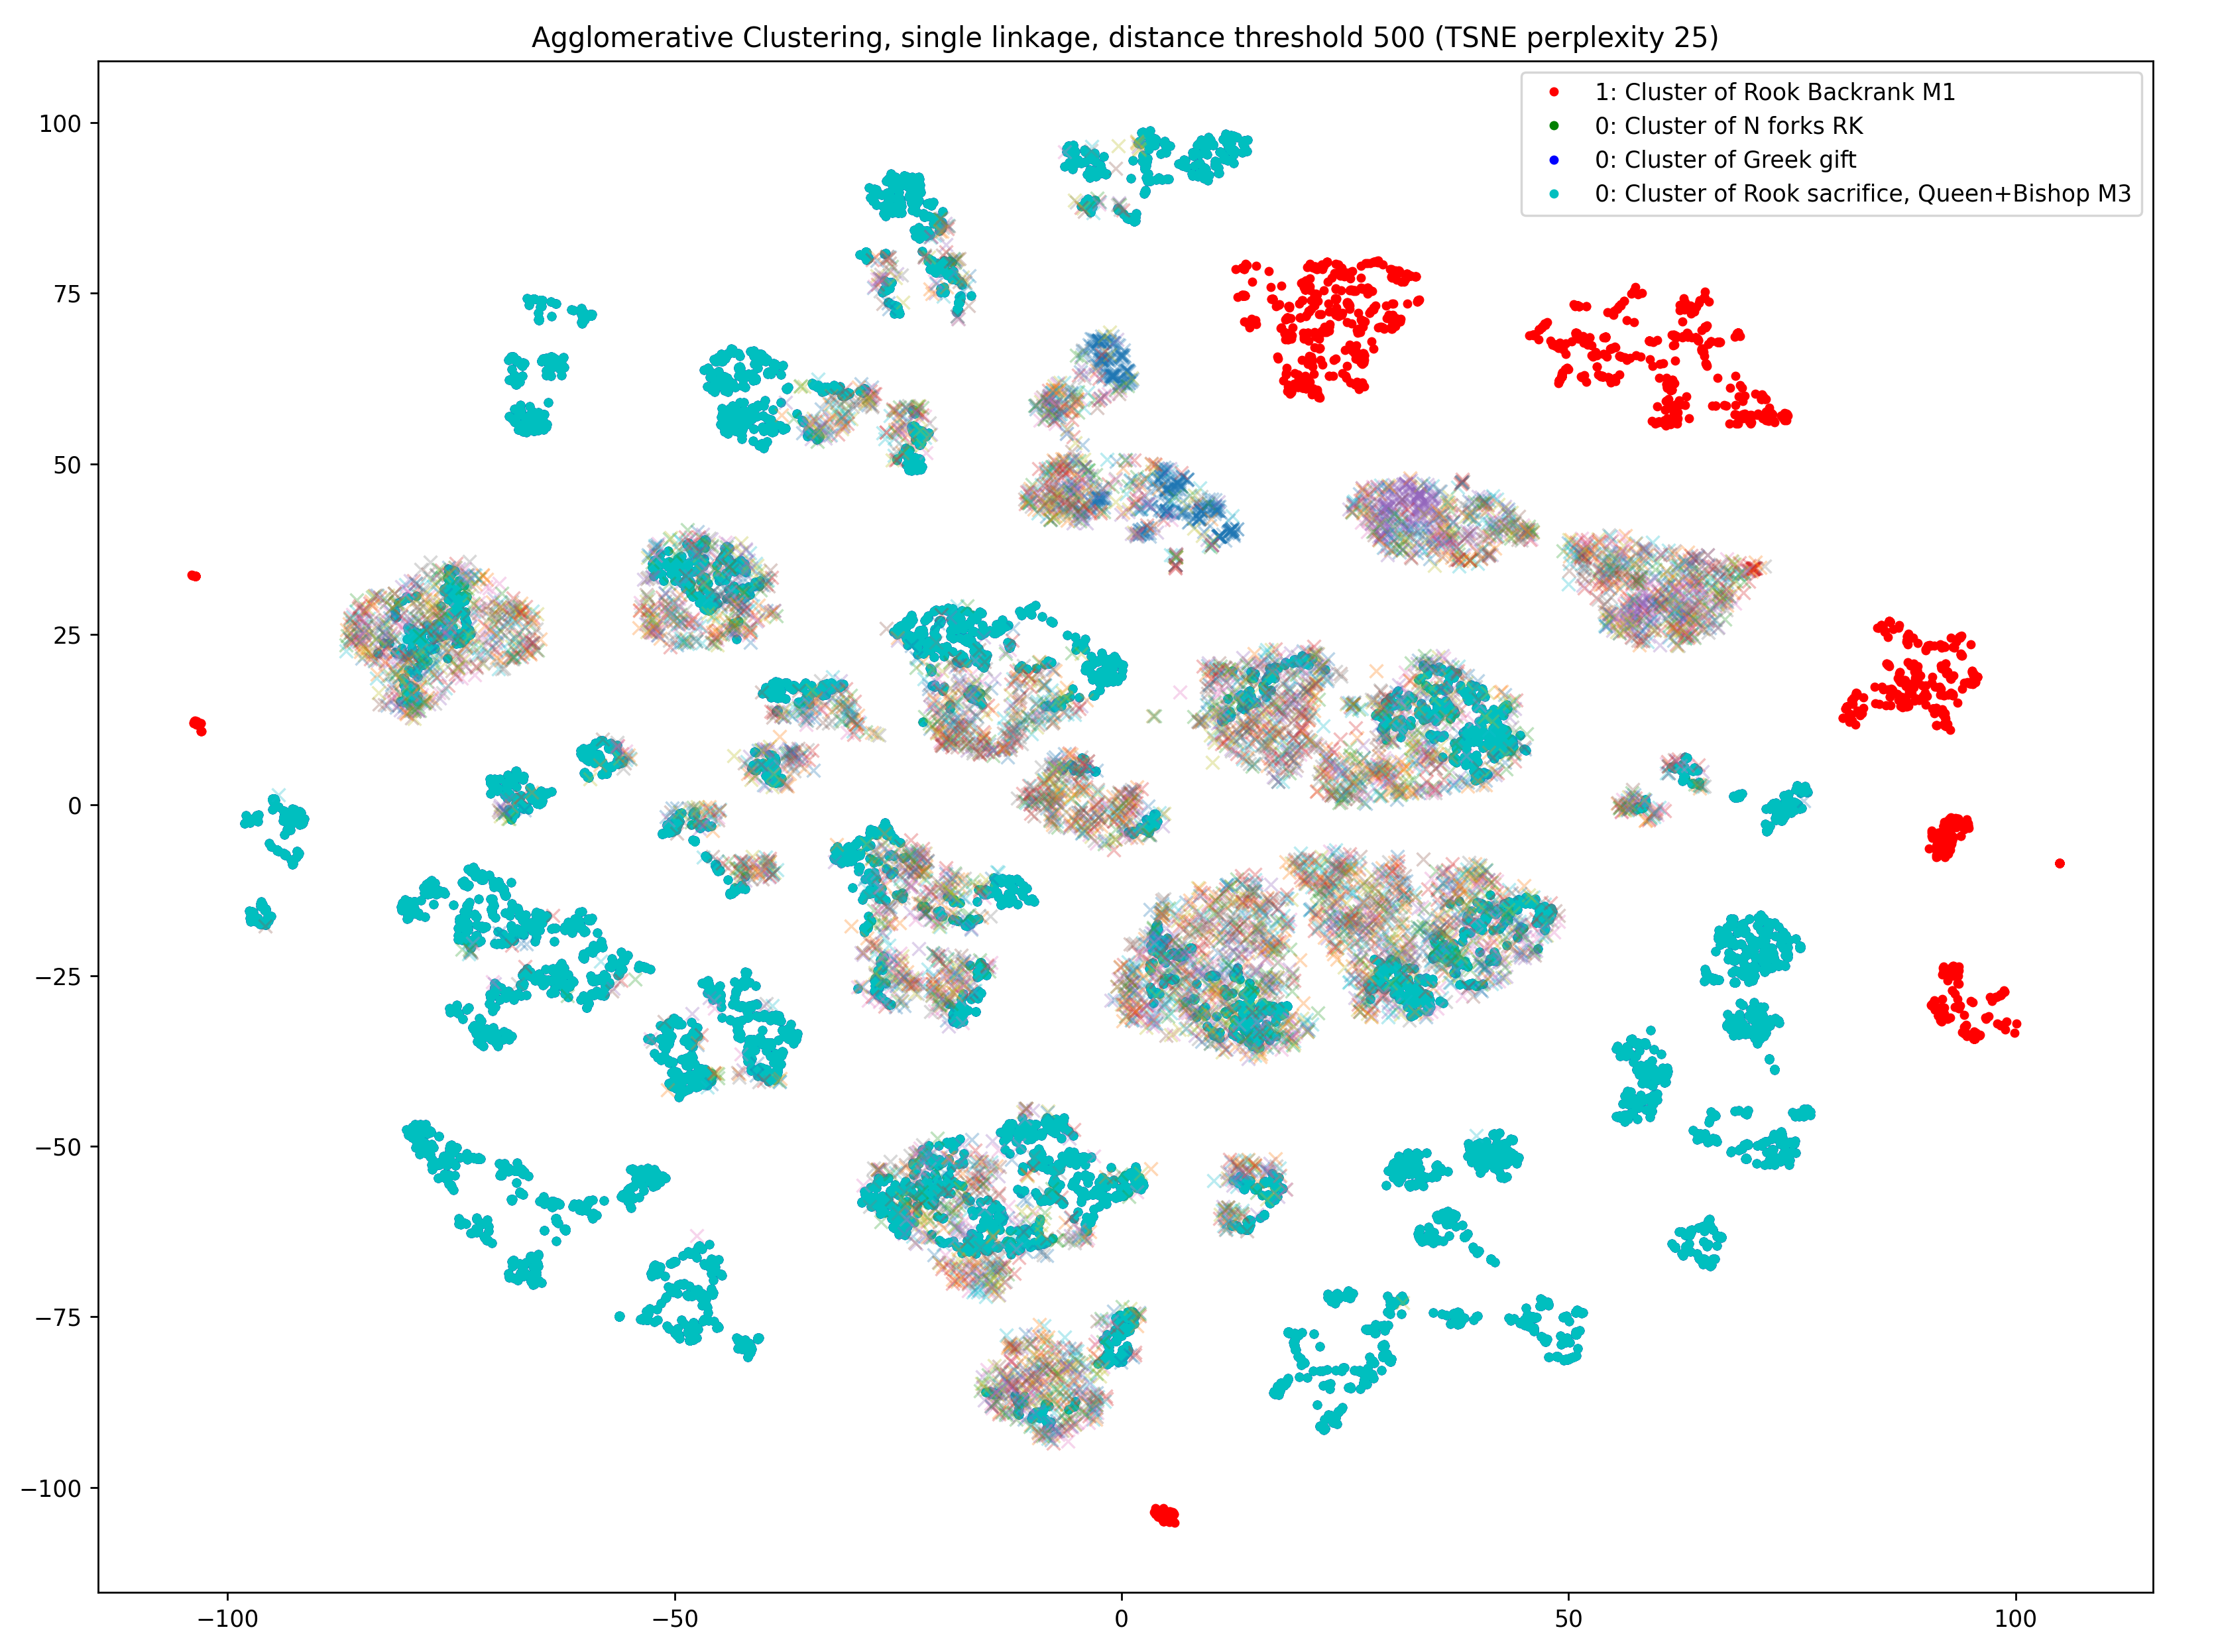
\includegraphics[width=0.9\textwidth]{project/img/tsne/ac_25.png}
  \caption{Agglomerative Clustering (single linkage, distance threshold $500$)}
  \label{tsne1}
\end{figure}

\begin{figure}[H]
  \centering
  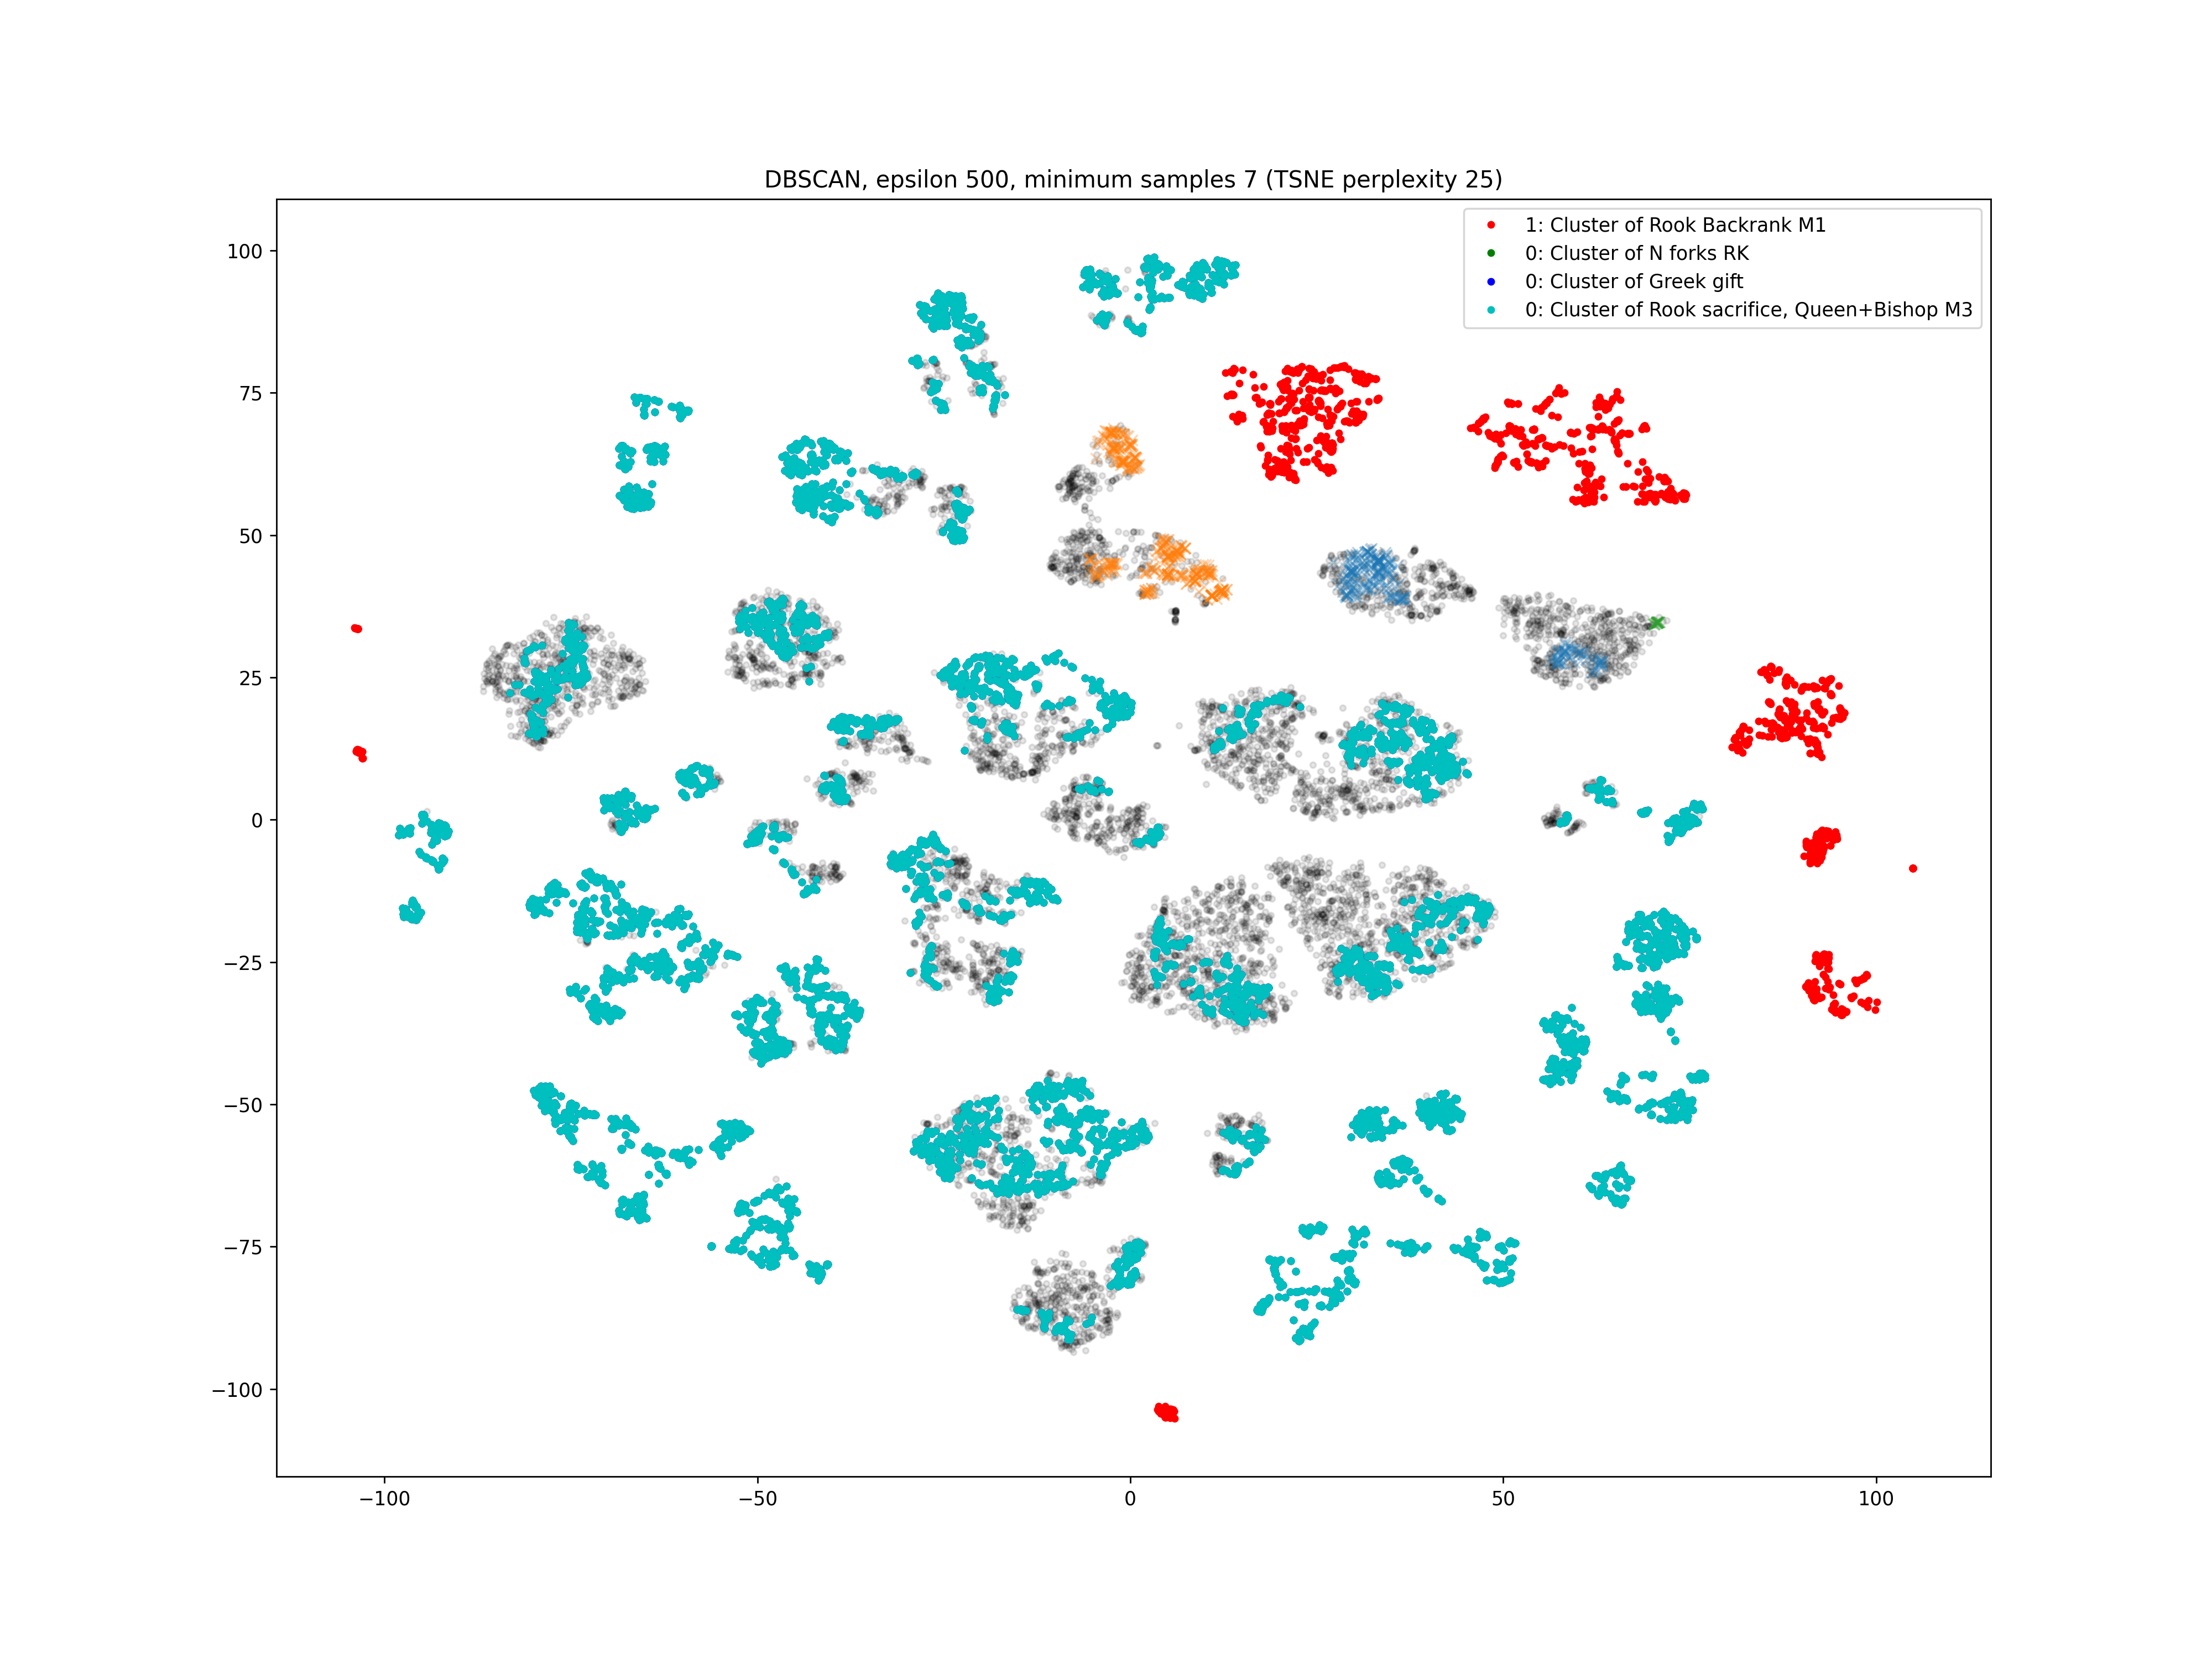
\includegraphics[width=0.9\textwidth]{project/img/tsne/dbscan_500_25.png}
  \caption{DBSCAN, $\epsilon=500$, minimum samples $7$.}
  \label{tsne2}
\end{figure}

\begin{figure}[H]
  \begin{minipage}[t]{0.475\textwidth}
    \centering
    \chessboard[setfen= 2rr2k1/ppb3pp/8/3p1q2/1P1Qn2P/P2KP2p/1B6/2RR4 w - -
    2 32]
    \caption{Puzzle in the same cluster as the \emph{back-rank mate-in-one}
    puzzle (\Cref{chess11}). Solution: \texttt{1.Qxg7\#}}
    \label{dbscanCluster11}
  \end{minipage}
  \hspace{0.05\textwidth}
  \begin{minipage}[t]{0.475\textwidth}
    \centering
    \chessboard[setfen= r3k2r/pp1qbppp/2pp1n2/8/3QP3/2N2P1P/PPP2P2/R1B3RK b
    kq - 4 13]
    \caption{Puzzle in the same cluster as the \emph{back-rank mate-in-one}
    puzzle (\Cref{chess11}). Solution: \texttt{1...Qxh3\#}}
    \label{dbscanCluster12}
  \end{minipage}
\end{figure}

\begin{figure}[H]
  \begin{minipage}[t]{0.475\textwidth}
    \centering
    \chessboard[setfen=8/8/1p3k2/p6p/P3K1pP/1P4P1/8/8 w - - 5 46]
    \caption{Puzzle from the endgame cluster. Both sides' pawns are frozen:
    they are either unable to move, or moving would cause them to be captured,
    creating a passed pawn for the opponent and losing the game. White wins
    with \texttt{1.Kf4}, getting \emph{opposition}, shouldering the black king
    away from the \texttt{h5} pawn.}
    \label{dbscanCluster13}
  \end{minipage}
  \hspace{0.05\textwidth}
  \begin{minipage}[t]{0.475\textwidth}
    \centering
    \chessboard[setfen=5k2/1N3ppp/n3p3/P7/5P2/6P1/7P/6K1 b - - 0 33]
    \caption{Puzzle from the endgame cluster. \texttt{1...Ke7} traps the
    knight(!), which is captured by the black king a few moves later.}
    \label{dbscanCluster14}
  \end{minipage}
\end{figure}

\begin{figure}[H]
  \centering
  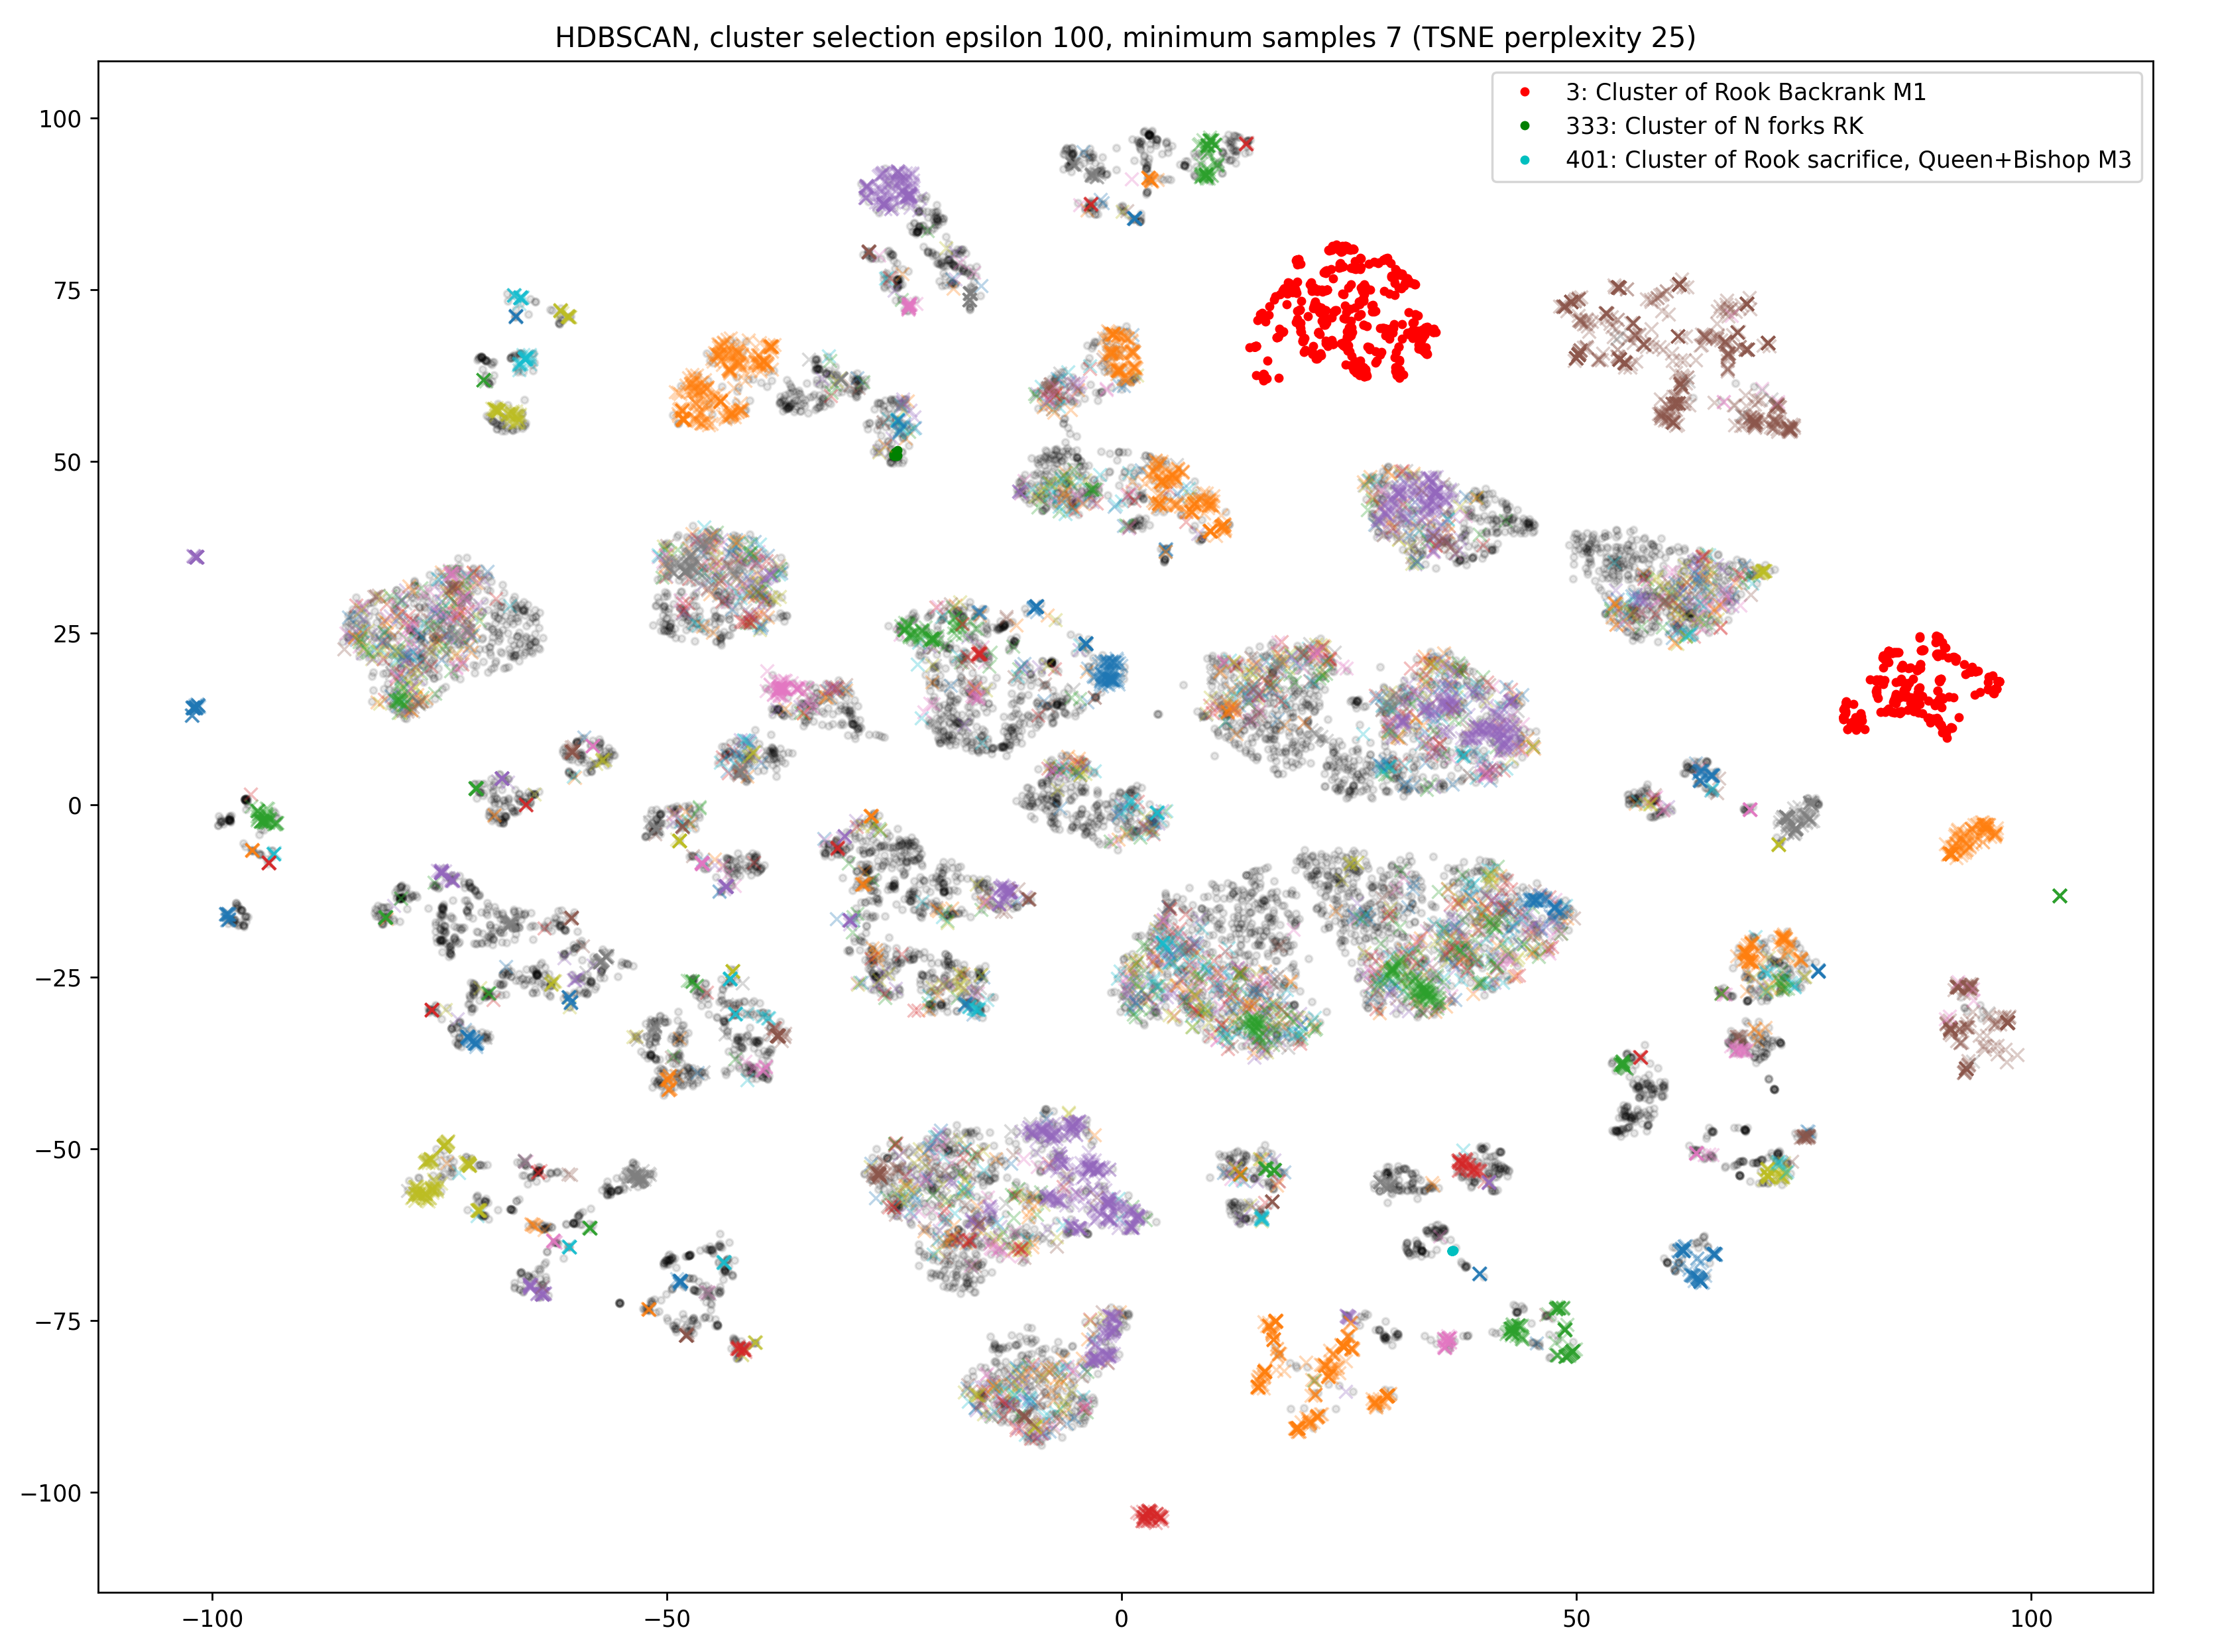
\includegraphics[width=0.8\textwidth]{project/img/tsne/hdbscan_2_25.png}
  \caption{HDBSCAN, cluster selection $\epsilon=100$, minimum samples $7$.}
  \label{tsne3}
\end{figure}

HDBSCAN puzzle clustering (\Cref{tsne3}) breaks up the megacluster which was
present in the previous two examples, while also producing a few other
promising clusters. In total, there are 420 clusters, with a mean cluster size
of $22.82$. Unfortunately, the \emph{Greek gift} puzzle (\Cref{chess13}) is
outside of any clusters, which is surprising, given the apparent effectiveness
of this algorithm.

Despite this, the clustering seems to perform much better than the former
attempts, and yields useful results. Cluster 333, under which the \emph{knight
fork} puzzle (\Cref{chess12}) falls, contains 18 puzzles, of which 17 are
tagged with `short' and 15 with `fork'. Two further puzzles are taken from this
cluster (\Cref{hCl1,hCl2}). Interestingly, the puzzle in \Cref{hCl2} is
not tagged as a `fork', even though it undeniably forks the king and bishop.
The remaining puzzles with no `fork' tag in this cluster have been manually
checked and are indeed knight forks. This is a good result, as it shows that
this method can pick up on themes that the Lichess puzzle database missed.

Another cluster of 61 puzzles was also found, 56 of which are tagged as
`endgame', a further 37 as `rook endgame', and none feature a `mate'. This
cluster appears to contain various rook and pawn endgames, where the opposing
side offers a rook trade. Accepting the trade is the only winning move for the
side solving the puzzle, and this cluster contains the puzzles with this theme.
An easy example (\Cref{chess15}) and a complex example (\Cref{chess16}) from
this cluster are featured.

These clusters are very interesting to analyse, as this method can pick up on
puzzle similarity that is not immediately obvious. During experimentation, it
was found that a larger distance matrix drastically improves the clustering
performance; this is likely because there are more examples of niche tactical
patterns, which means they can be clustered together. Without enough examples,
many of these puzzles are categorised as as noise/outliers: approximately 50\%
(\Cref{tabHDBSCAN}). 

If a larger distance matrix can be constructed, it is likely that the
clustering method will improve more, and allow finer categorisation of puzzles.
The resource and time commitment to do so unfortunately prohibited this.

\begin{figure}[H]
  \begin{minipage}[t]{0.475\textwidth}
    \centering
    \chessboard[setfen=3r2r1/PR6/2pk2p1/1p1p1nP1/3PnPQ1/1PP1P3/2K5/5R2 b -
    - 0 39]
    \caption{Puzzle from the \emph{knight fork} cluster. Black forks with
    \texttt{1...Nxe3+}, hitting two major pieces at once.}
    \label{hCl1}
  \end{minipage}
  \hspace{0.05\textwidth}
  \begin{minipage}[t]{0.475\textwidth}
    \centering
    \chessboard[setfen=
    rn1q1b1r/pp3kpp/2p2n2/4p3/4p1b1/2NP1N2/PPP2PPP/R1BQK2R w KQ - 0 8]
    \caption{Puzzle from the \emph{knight fork} cluster. White wins a bishop
    after \texttt{1.Nxe5+}.}
    \label{hCl2}
  \end{minipage}
\end{figure}

\begin{figure}[H]
  \begin{minipage}[t]{0.475\textwidth}
    \centering
    \chessboard[setfen=8/8/k5r1/p5R1/5K2/P7/8/8 b - - 1 51]
    \caption{Rook trade cluster. After \texttt{1...Rxg5 2.Kxg5 Kb5}, Black wins
    the remaining white pawn and shoulders the white king for a victory.}
    \label{chess15}
  \end{minipage}
  \hspace{0.05\textwidth}
  \begin{minipage}[t]{0.475\textwidth}
    \centering
    \chessboard[setfen=8/2p4p/1k4p1/p1r5/2R4P/1P2K3/P4P2/8 b - - 3 47]
    \caption{Complex position in the rook trade cluster. \texttt{1...Re5+} is
    tempting, and was played in the game where this position occured. This,
    however, loses the advantage. After trading rooks, \texttt{1...Rxc4
    2.bxc4}, Black threatens to win the \texttt{c4} pawn with \texttt{2...Kc5
    3.Kd3 Kb4}, allowing Black to capture the \texttt{a2} pawn. The white king
    cannot trap the black king on the \texttt{a} file as both sides quickly run
    out of pawn moves. With correct play, White is forced into
    \emph{zugzwang}.}
    \label{chess16}
  \end{minipage}
\end{figure}

\pagebreak

\section{$k$-Nearest Neighbours}\label{treeS3}

Since the unsupervised clustering method (\Cref{treeS2}) produces too many
outliers to be useful for inference, a classic $k$-nearest neighbours ($k$-NN)
approach \citep{fix1985discriminatory} can be used both for classification of
puzzle themes and regression of puzzle difficulty rating.

It has been shown that the novel distance function (\Cref{treeS13}) has
promising results for finding similar positions to a given puzzle
(\Cref{treeS21}), so with the appropriate setup, this method should be viable
for inference and comparison to the deep learning (\Cref{mlChapter}) method.

\subsection{Label Prediction and Difficulty Regression with $k$-NN}

The process of predicting a label and difficulty for an unseen chess puzzle is
straightforward. Given a puzzle, its $k$ nearest neighbours in the known
(training) dataset are found. If half or more of the neighbours are tagged with
a certain tactic label, the puzzle is predicted to have that label. The puzzle
difficulty is the mean of the difficulty of the neighbours.

\subsection{Search for the Best $k$}\label{treeS31}

One of the downsides of $k$-NN is the slow inference performance. This makes
tuning the parameter $k$ difficult, as the running time is roughly proportional
to the multiple of the training set size and validation set size. To address
this, random subsets of the training and validation sets (\Cref{mlS12}) of size
20,000 each were used. This amount showed acceptable clustering performance
(\Cref{treeS22}), so it will provide a reasonable starting point for this
approach.

Paramater $k$ was varied from $1$-$100$. The results (\Cref{knn}) show that
$k=24$ is optimal for label prediction, with an average of $2.8011$ incorrect
labels (includes both false positives and false negatives). For difficulty
regression, $k=22$ is best, with an average mean squared difficulty rating
error of $\sim\!434.0^2$. 

Even though different $k$ values for the two tasks are possible, $k=24$ was
chosen for both label prediction and difficulty regression, as it simplifies
implementation and as a trade-off, increases difficulty regression error to
$\sim\!434.3^2$ -- a negligible difference. 

\begin{figure}[H]
  \centering
  
\includegraphics[width=0.9\textwidth]{project/img/knn.png}
  \caption{Effect of $k$ on label prediction and difficulty regression performance.}
  \label{knn}
\end{figure}


\chapter{Evaluation}
\chapter{Conclusion}

\section{Related Work}

\subsection{A Language For Encoding Piece Relationships}

\citet{chessLanguage} describe a language to search across chess positions. The
main features of this language are descriptions for a chess piece
attacking/defending another, attacking/defending a square, being located at a
square, a square not being available for the enemy king, and the structure of
white/black pawns on the board.v

With their novel language, they are able to search a chess database for a
pre-determined pattern, such as the \emph{Greek gift sacrifice}, defined in the
language as `\texttt{kg8, pf7, pg7, B(ph7), Nf3, Qd1, Pe5}. With inspiration
from the FEN notation, this string corresponds to a black king on g8
(\texttt{kg8}), black pawns on f7, g7; a white bishop attacking a black pawn on
h7 (\texttt{B(ph7)}), a white knight on f3 (ready to deliver a check with
\texttt{Ng5+}, a common motif in \emph{Greek gift sacrifices}), a white queen
on d1 (\texttt{Qd1}), and finally, a white pawn on e5 (\texttt{Pe5}),
dislodging the usual black knight on f6.

This returns positions such as the one in Figure \ref{chess3}. After
\texttt{16...Be7 17. O-O}, Black blundered with \texttt{17...Bxa3??}, after
which, a \emph{Greek gift sacrifice} (\texttt{18.Bxh7!}, shown in Figure
\ref{chess4}) was made, eventually leading to a win for White.

\begin{figure}[H]
    \begin{minipage}{0.475\textwidth}
        \centering
        \chessboard[setfen=r1b2rk1/qp3ppp/p1n1pb2/4P3/3P4/P1BB1N2/5PPP/1R1QK2R
        b K - 0 16]
        \caption{\textbf{Pirc, V -- Porreca, G}, YUG-ITA m 1953, move 16.}
        \label{chess3}
    \end{minipage}
    \hspace{0.05\textwidth}
    \begin{minipage}{0.475\textwidth}
        \centering
        \chessboard[setfen=r1b2rk1/qp3ppB/p1n1p3/4P3/3P4/b1B2N2/5PPP/1R1Q1RK1 b
        - - 0 18]
        \caption{\textbf{Pirc, V -- Porreca, G}, YUG-ITA m 1953, move 18. Black
        resigned after 6 moves.}
        \label{chess4}
    \end{minipage}
\end{figure}

Their language is also able to deal with some light variations, as it is able
to identify the games shown in Figures \ref{chess5}, \ref{chess6}. In both of
these positions, White has the brilliant move \texttt{1.Qh6+!!}, following with
\texttt{2.Rh8\#} if \texttt{1...Kxh6}, and either \texttt{2.Rf7\#} or
\texttt{2.Rb7+} (leading to a quick mate) if \texttt{1...gxh6}. 

This pattern, whilst very rare, is undeniably identical between the 2 games.
The unavailability of the \texttt{g6} square to the enemy king, combined with
the harmony of White's pieces leads to the same tactic in both games.

\begin{figure}[H]
    \begin{minipage}{0.475\textwidth}
        \centering
        \chessboard[setfen=2R5/4bppk/1p1p4/5R1P/4PQ2/5P2/r4q1P/7K w - - 5 50]
        \caption{\textbf{Carlsen, M -- Karjakin S}, World Chess Championship
        2016, move 50.}
        \label{chess5}
    \end{minipage}
    \hspace{0.05\textwidth}
    \begin{minipage}{0.475\textwidth}
        \centering
        \chessboard[setfen=5R2/bp4pk/2n3p1/P7/P1q3bP/6P1/3Q3K/1R6 w - - 1 32]
        \caption{\textbf{Popov, N -- Novopashin, A}, URS-ch otbor 1979, move
        32.}
        \label{chess6}
    \end{minipage}
\end{figure}

The work of \citet{chessLanguage} is a promising proof of concept that shows
the power of a language that allows to specify piece relationships on a more
abstract level than previously possible. The biggest drawback of their
solution, as mentioned by the authors, is the fact that this language still
requires an expert with pre-existing extensive knowledge to encode the tactics
into their language.

\subsection{CQL: Chess Query Language}

The Chess Query Language (CQL), invented by \citet{cql}, is another
implementation of an advanced way to find chess positions in a given database.
Since its inception in 2004, it has grown and is able to support very powerful,
sometimes esoteric, queries to find predefined patterns.

An example of such a query is provided on the CQL website \citep{cqlSmothered},
and is shown in Figure \ref{cql} for reference. In this query, \texttt{btm}
means `black-to-move` and \texttt{mate} means checkmate is played. This
language is incredibly powerful and terse, as it allows specifying complicated
piece relationships and supports quality-of-life features such as matching
mirror positions or reversed-colour positions.

\begin{figure}[H]
    \centering
    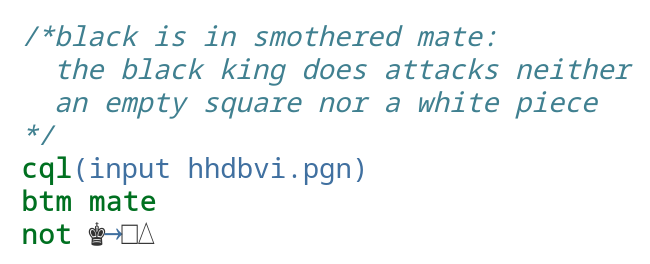
\includegraphics[width=0.45\linewidth]{background/img/cql.png}
    \caption{A CQL query to find positions where smothered mate occured.}
    \label{cql}
\end{figure}

In addition to Costeff's CQL, there exists a from-scratch clone of CQL6
\citep{cqli} which includes extra features and supports other chess variants.

\subsection{Chess Moves As Kernels For Texture Classification}

In this study, \citet{chessKernel} propose novel kernels for efficient feature
extraction in the task of texture detection. These 5x5 kernels are directly
based on the move a rook, bishop, knight, and their combinations. 

Whilst not directly applicable to the context of chess puzzle analysis, this
work shows that it may be possible to include these kernels in an CNN-based
analysis of the chess position. It would be interesting to apply to the other
CNN chess work (e.g. \citeauthor{chessCNN}'s thesis, discussed in Section
\ref{chessCNNSection}) and analyse its effect on the success of the technique.

\subsection{The Chess Transformer: Mastering Play using Generative Language
Models}

\citet{chessTransformer} demonstrate the ability of transformers to learn the
rules of chess and complex gameplay by analysing PGN games with a fine-tuned
GPT-2 transformer. By treating PGN games as a sequence of natural language
words, the authors show successful results and are able to generate new games
without specifying chess rules.

A key downside of their work is that their model generates illegal moves, which
have to be filtered manually using a chess library \citep{chessTransformer}.
This `hallucination' effect is a downside of using transformers, and other
generative techniques, in chess. 


%\appendix
\chapter{First Appendix}

\bibliographystyle{unsrtnat}
\bibliography{bibs/bibliography}

\end{document}
